\documentclass[12pt]{article}

% Basic stuff
\usepackage{fullpage}
\usepackage{graphicx}
\usepackage[parfill]{parskip}
\usepackage[utf8]{inputenc}

% Skip one line between paragraphs
\parskip1em
 
% Standard things to include for math   
\usepackage{amsmath,amssymb,amsfonts,amsthm,mathrsfs}

% Other stuff
\usepackage{wasysym}
\usepackage{stmaryrd}
\usepackage{hyperref}
\usepackage{datetime} \usdate
\usepackage[shortlabels,inline]{enumitem}
\usepackage{changepage}
\usepackage{tcolorbox}
\usepackage{tikz}
\usepackage{xcolor}
\hypersetup{
    colorlinks,
    linkcolor={red!50!black},
    citecolor={blue!50!black},
    urlcolor={blue!80!black}
}


% Some of Ebrahim's definitions
%\newcommand{\note}[1]{[#1]}
\newcommand{\note}[1]{[This portion has yet to be written.]}
\newcommand{\done}{\\\hspace*{0pt}\hfill$\blacksquare$}
\def\N{\mathbb{N}}
\def\R{\mathbb{R}}
\def\Q{\mathbb{Q}}
\def\Z{\mathbb{Z}}
\def\e{\varepsilon}
\def\d{\delta}
\newcommand{\seq}[1]{\left(#1\right)_{n\in\N}}
\renewcommand{\emptyset}{\{\hspace{-2pt}\}}
\newcommand{\powerset}[1]{\mathcal{P}(#1)}
\newcommand{\dom}[1]{\operatorname{dom}(#1)}
\newcommand{\ran}[1]{\operatorname{ran}(#1)}
\newcommand{\rev}[1]{{#1}^{\dashv}}
\newcommand{\drev}[1]{{#1}^{\dashv\dashv}}
\newcommand{\injrightarrow}{\xrightarrow{\text{inj}}}
\newcommand{\surjrightarrow}{\xrightarrow{\text{surj}}}
\newcommand{\bijrightarrow}{\xrightarrow{\text{bij}}}
\newcommand{\AND}{\wedge}
\newcommand{\OR}{\vee}
\newcommand{\ARR}{\Rightarrow}
\newcommand{\DARR}{\Leftrightarrow}
%\newcommand{\REL}{\leadsto}
\newcommand{\REL}{\sim}
\newcommand{\CLASS}[2]{[#1]_{#2}}

\def\bbel{
\,
\raisebox{-2pt}{
\includegraphics[scale=0.8]{bbel.pdf}}
\,
}

\newcommand{\ALL}[2]{\left(\,\forall{#1}\,\bbel\,#2\,\right)}
\newcommand{\EXIST}[2]{\left(\,\exists{#1}\,\bbel\,#2\,\right)}
\newcommand{\COLL}[2]{\left\{\, {#1} \,\bbel\, {#2} \, \right\}}
\newcommand{\settext}[2]{\COLL{#1}{\text{#2}}}
\newcommand{\SUB}[1]{\mathcal{P}(#1)}
\newcommand{\occ}[1]{\operatorname{occ}(#1)}
\newcommand{\id}[1]{\textrm{id}_{#1}}
\renewcommand{\next}[1]{\operatorname{next}({#1})}
\newcommand{\addone}{\ddag}

\DeclareFontFamily{OT1}{pzc}{}
\DeclareFontShape{OT1}{pzc}{m}{it}{<-> s * [1.10] pzcmi7t}{}
\DeclareMathAlphabet{\mathpzc}{OT1}{pzc}{m}{it}
\newcommand{\add}{\mathpzc{ADD}}

\newcommand{\eqnm}{\approx} % equinumerous
\newcommand{\injex}{\preceq} % an injection exists
\newcommand{\injnobij}{\prec} % an injection exists but no bijection exists

%\newcommand{\SUBST}[3]{{#1}\left[{#2}\mapsto{#3}\right]}
%\newcommand{\SUBST}[3]{{#1}_{{#2}\mapsto{#3}}}
\newcommand{\SUBST}[3]{{#1}_{[{#2}\rightarrow{#3}]}}
%\newcommand{\SUBST}[3]{{#1}\,\text{replacing}\,{#2}\,\text{by}\,{#3}}
%\newcommand{\SUBST}[3]{{#1}\ \text{replacing}\ {#2}\ \text{by}\ {#3}}

%\newcounter{exercise}[subsection]
\newcounter{exercise}
\newcounter{rule}
\newcounter{theorem}
%\def\theexercise{\thesubsection.\arabic{exercise}}

\def\putExerciseHeading{\refstepcounter{exercise} \textbf{Exercise \theexercise}}
\def\putRuleNumber{\refstepcounter{rule}\therule}
\def\putThmNumber{\refstepcounter{theorem}\thetheorem}

\newcommand{\ex}[1]{ \putExerciseHeading: #1}
\newcommand{\indented}[1]{\begin{adjustwidth}{1em}{}#1\end{adjustwidth}}


\def\thmcolonspace{\hspace{0.2em}}
\def\proofnewline{\\[0.75em]} % Separates theorem box from proof, no new paragraph expected.
\def\thmStartNewline{\\[0.3em]} % Vertically separates theorem heading from theorem statement, sometimes used.
\def\proofsep{\\[-0.5em]} % Separates different proofs (e.g. to diff parts of same theorem). No new paragraph expected.
\renewcommand\qedsymbol{$\blacksquare$}
\def\done{\qed\\[0em]} % QED with newline so that QED symbol is flushed to the right. IDK why newline is needed for this to happen.
\newcommand{\thmbox}[1]{\fbox{\parbox{\textwidth}{{#1}}}}
\newcommand{\THMMOCK}[2]{\thmbox{\textbf{Theorem:} \thmcolonspace #1} \proofnewline \textit{Proof:} #2\done}
\newcommand{\THMP}[2]{\thmbox{\textbf{Theorem \putThmNumber:} \thmcolonspace #1} \proofnewline\textit{Proof:} #2\done}
\newcommand{\THMPL}[3]{\thmbox{\textbf{Theorem \putThmNumber{#3}:} \thmcolonspace #1} \proofnewline\textit{Proof:} #2\done}
\newcommand{\THMNP}[3]{\thmbox{\textbf{Theorem \putThmNumber\ (#1):} \thmcolonspace #2} \proofnewline\textit{Proof:} #3\done}
\newcommand{\THM}[1]{\thmbox{\textbf{Theorem \putThmNumber:} \thmcolonspace #1}}
\newcommand{\THMN}[2]{\thmbox{\textbf{Theorem \putThmNumber\ (#1):} \thmcolonspace #2}}
\newcommand{\AXIOM}[1]{\thmbox{\textbf{Axiom \putThmNumber:} \thmcolonspace #1}}
\newcommand{\AXIOMN}[2]{\thmbox{\textbf{Axiom \putThmNumber\ (#1):} \thmcolonspace #2}}
\newcommand{\DEFN}[2]{\thmbox{\textbf{Definition \putThmNumber\ (#1):} \thmcolonspace #2}}
\newcommand{\DEF}[1]{\thmbox{\textbf{Definition \putThmNumber:} \thmcolonspace #1}}


\newcommand{\RULE}[2]{\begin{tcolorbox}[title=Rule \putRuleNumber: #1,colbacktitle=white,coltitle=black,colback=white]#2\end{tcolorbox}}
\newcommand{\DRULE}[2]{\begin{tcolorbox}[title=Derived Rule \putRuleNumber: #1,colbacktitle=white,coltitle=black,colback=white]#2\end{tcolorbox}} % IDK if derived rules will be different
\newcommand{\DRULEPF}[3]{\begin{tcolorbox}[title=Derived Rule \putRuleNumber: #1,colbacktitle=white,coltitle=black,colback=white] {#2} \tcblower \textbf{Proof:} {#3} \end{tcolorbox}}
\newcommand{\DRULEPZ}[2]{\begin{tcolorbox}[title=Derived Rule \putRuleNumber: #1,colbacktitle=white,coltitle=black,colback=white] {#2} \tcblower \textbf{Proof:} 
                         \putExerciseHeading. \end{tcolorbox}}

\def\pA{\Phi}
\def\pB{\Psi}
\def\pC{\Omega}
\def\pD{\Sigma}
\def\pE{\Gamma}
\def\pF{\Delta}




\begin{document}

\begin{center} {\Large \scshape Mathematical Proofs and Mathematical Writing}
\end{center}
(compiled on \today\ at\ \currenttime)
\hfill

\tableofcontents

\paragraph{Layout}
Section \ref{sec:logic} will develop mathematical logic and show you how logical arguments factor into writing.
We will not yet have anything to argue \emph{about}, so our ``proofs'' in section \ref{sec:logic} will be about nothing in particular.
Section \ref{sec:sets} will then give some mathematical objects to talk about, and we will then put
content into the empty skeleton arguments of section \ref{sec:logic}.
Section \ref{sec:sets} will take you from the axioms of set theory up through a construction of the natural numbers and more.
We start in section \ref{sec:lang} with an introduction to formal axiomatic systems and informal proofs.

\section{Mathematical Language}
\label{sec:lang}

%\note{what to put here:
%this course is about both set theory and writing.
%set theory is axiomatic. describe what i mean by that, why we would do that, and the historical relevance of it.
%why rigor anyway?
%logic can also be done this way, but we will not.
%we will follow a more intuitive and informal writing-focused approach for logic,
%saving our rigor-enegery for set theory.
%perhaps include a discussion levels of rigor and formality, with one level relegating the rigor to other levels.
%mention the importance of writing and the roughness of this transition for many people.
%mention the value of forgetting what you knew before, but not really forgetting it all.}
%an illustration containing two towers, one of the math t hey built up till now, and one new tower starting here of the math they are now building
%a comment on hyperlinks in this document and the usefulness of having a back button


%\note{Write the general intro here later.}





\subsection{Parts of Speech}
\label{sec:parts_of_speech}

In a language, a \emph{part of speech} is a collection of words that share grammatical properties.
For example here are some common English parts of speech: pronouns, nouns, verbs, adjectives, and adverbs.
Different languages can have different parts of speech that are useful for describing their grammar.
To build up the grammar of a language, one can specify how parts of speech fit together to form larger
\emph{constituents}, such as noun phrases and clauses. One can further describe how
constituents fit together to form even more complex constituents, eventually grammatical sentences.

Mathematics is a language, and so it makes sense to build up its grammar (its \emph{syntax}) using this same strategy.
Instead of pronouns, nouns, verbs, noun phrases, sentences, and so on, there are just four constituents in
mathematics. Two are basic parts of speech and two are more complex constituents:
\begin{itemize}
\item \emph{Variables} are a basic part of speech.
\item \emph{Constants} are a basic part of speech.
\item \emph{Terms} can be built out of variables, constants, other terms, and propositions.
\item \emph{Propositions} can be built out of variables, constants, terms, and other propositions.
\end{itemize}

Let's go through each of these in detail.

\def\sp{\hspace{1em}}
\paragraph{Variables}
Variables serve as placeholders, waiting to be replaced by other symbols.
They are most like pronouns in English.
For example the pronoun ``it'' is a placeholder referring to something in a discussion, but what it refers to depends on the context of the discussion.
Variables are like that.
Here are some variables:
\begin{center}
$a$ \sp $b$ \sp $A$ \sp $f$ \sp $q$ \sp $x$\sp $\alpha$\sp $\beta$
\end{center}
Variables are copies of letters coming from an alphabet (usually Latin or Greek) and written in ink/chalk/pixels.



\def\sp{\hspace{1em}}
\paragraph{Constants}
\hypertarget{hl:constants}{Constants} are used as fixed names for specific mathematical objects.
They are most like \emph{proper} nouns in English.
Here are some constants:
\begin{center}
$0$ \sp $1$ \sp $2$ \sp $3$ \sp $4$ \sp $5$ \sp $6$ \sp $7$ \sp $8$ \sp $9$ \sp $\N$ \sp $\R$ \sp $\emptyset$
\end{center}
The difference between constants and variables is that constants are not meant to be substituted for.
The constant ``$2$'' refers to a specific thing, rather than being a placeholder for something.


Note that we are mainly talking about \emph{elements of language}, and not about what those elements \emph{refer} to.
Germany is not a noun, it's a country. ``Germany'' is, however, a noun.
Similarly, we can say that $2$ is not a constant, but rather ``$2$'' is.
And $x$ is not a variable, but rather ``$x$'' is.
Quotation marks help us make the distinction between a symbol and what the symbol refers to
(though I will often be lazy and drop the quotation marks).




\def\sp{\hspace{1em}}
\paragraph{Terms}
Terms are strings of marks (expressions) that refer to \emph{mathematical objects}.
Since variables and constants refer to mathematical objects, they are special cases of terms.
But you can also have more complicated terms that are built out of simpler ones.
Terms are most like \emph{noun phrases} in English.
For example the phrase ``the cup that you drank from'' is a noun phrase;
it doesn't make any assertion but rather it just refers to a \emph{thing}.
Here are some terms:
\begin{itemize}[label=\sp]
\item $x$
\item $7$
\item $\{2,3,a,7\}$
\item $f(x)$
\item $\{(z,w)\} \circ g$
\item $S\times Q$
\item the square of the seventh prime number
\item a triangle
\item twelve dimensional euclidean space
\item the collection of even integers
\item $\settext{n}{$n\in\Z$ and $n$ is even}$
\item $\settext{n}{$(n\in\Z)\AND (\exists k\,|\,(k\in\Z)\AND(2k=n))$}$
\end{itemize}
The last three terms actually refer to the same mathematical object; this will soon become clear
when we get into \emph{how} the symbols refer to objects (semantics). For now we are only looking at
\emph{which} strings of symbols \emph{can} refer to objects (syntax).
You can see that some terms are more ``symbolic,'' while others are more ``Englishy.''
The formal language of mathematics is purely symbolic,
but we almost never use the language in its purest form.
Typically, we communicate by some combination of English and mathematics.


\def\sp{\hspace{1em}}
\paragraph{Propositions}
Propositions are strings of marks (expressions) that \emph{make assertions}.
They are most like \emph{sentences} in English (declarative sentences).
Propositions can be true or false. 
Here are some propositions:
\begin{itemize}[label=\sp]
\item $x\in S$.
\item $5\notin x$.
\item $0=2$.
\item $(x\neq y) \AND (x\neq z) \AND (y\neq z)$.
\item $x$, $y$, and $z$ are distinct.
\item Either $A\subseteq P$ or $x\in S$, but not both.
\item $f:X\rightarrow Y$.
\item If $x\in S$, then we either have $x\notin W$ or we have $x\in\Z$.
\item $\neg(X\times Y \subseteq Z)$.
\item Every integer is even.
\item $\ALL{n}{(n\in\Z)\ARR \EXIST{k}{(k\in\Z)\AND(2k=n)}}$.
\end{itemize}
The last two propositions are actually saying the same thing, as we will see when we get into semantics.
Again, you can see that some propositions are more ``symbolic,'' while others are more ``Englishy.''
Typically, we make mathematical assertions by using some combination of English and mathematics.
The English that we use is a crude, but human-friendly, stand-in for formal mathematical statements.



\ex{
Determine whether each of the following is a term or a proposition.
\begin{enumerate}
\item $n$
\item $1+1=0$
\item $n$ is an odd integer
\item an odd integer
\item $f$ is a function with domain $S$
\item $1+(2+3)$
\item the empty set
\item the sum of two vectors is another vector
\item the zero vector
\item the evenness of $2$ % this one is a trick, it's neither unless you are doing metamathematics
\end{enumerate}
}

\subsection{Theorems and Proofs}

Mathematics is ultimately about propositions.
Propositions \emph{say} things, sometimes true things and sometimes false things.
We want to know: Which propositions are true? What does ``true'' even mean?
We will not exactly define ``true,'' but we will define ``provable,''
and provability will be our notion of truth.

The rules of logic allow us to make deductions and \emph{prove} new propositions
from already proven propositions.
Those already proven propositions themselves had to be proven via a sequence of logical deductions
that was applied to other previously proven propositions.
And so on...
but where does it all start?

\paragraph{Axioms}
Some propositions are declared to be \emph{axioms},
which makes them serve as starting points in our mathematical system.
The next paragraph will clarify this.

\paragraph{Proofs}
A \emph{proof} is a sequence of propositions such that each proposition is either
(1) an axiom, 
(2) an already proven proposition,
or, (3) the result of applying the rules of logic to \emph{previous} propositions in the sequence.
A proposition that appears in a proof is said to be \emph{proven}.


\paragraph{Theorems}
A \emph{theorem} is a proposition which is asserted to have a proof.



\def\ES{\settext{x}{$x\neq x$}}

\paragraph{Example}
Here is an example of a proof of the proposition ``$(\forall x\,|\,x\notin\ES)$'':
\begin{adjustwidth}{1cm}{}
$(x\in\ES)\Longrightarrow (x\neq x)$\\ 
$(x=x)\Longrightarrow (x\notin \ES)$\\
$x=x$\\
$x\notin\ES$\\
$(\forall x\,|\,x\notin\ES)$
\end{adjustwidth}
Do not worry about interpreting what the propositions are trying to \emph{say};
I just want to demonstrate how a theorem arises as a result of applying the rules of logic
to various axioms. What you see above is a sequence of five propositions, ending with the
one I claimed to be proving, namely ``$(\forall x\,|\,x\notin\ES)$''.
To really be convinced that we are looking at a proof, we would need a \emph{justification}
for each of the five propositions-- for each proposition we need to either point out that it is
an axiom, or we need to verify that it follows logically from the previous propositions.
In this example, two of the propositions are axioms, and the other three are logical deductions;
here is a schematic depiction of these relationships:
\begin{center}
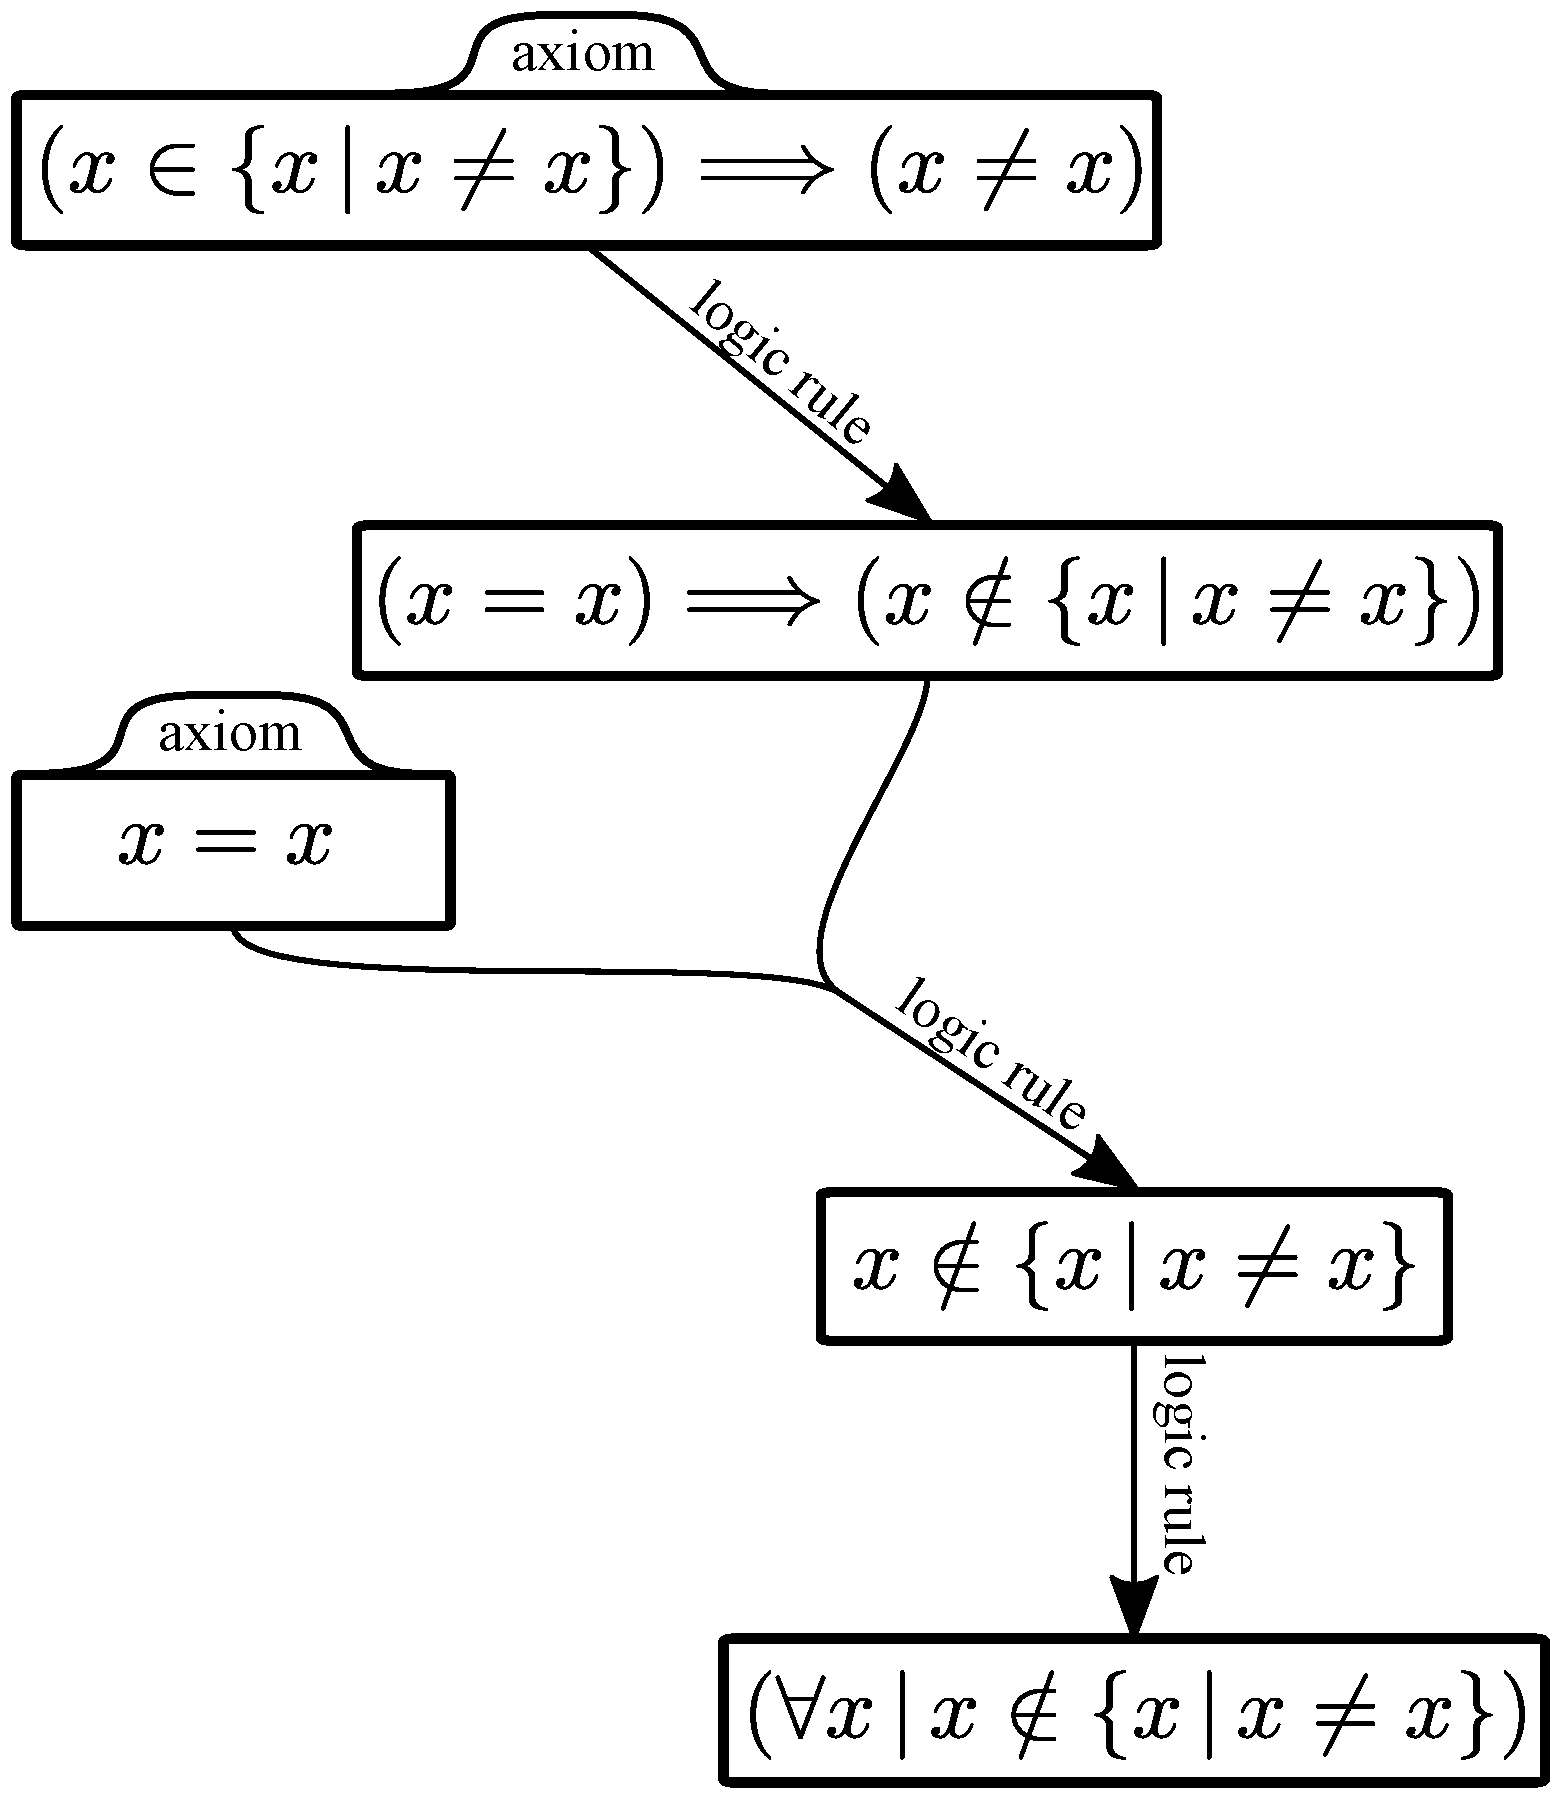
\includegraphics[scale=0.25]{img/proofFlow.pdf}
\end{center}
Again, don't worry yet about understanding why this works.
What I want you to take away from this is the general structure:
we have axioms serving as starting propositions, and we use logic to ``flow'' out from
the starting points and prove other propositions.

Given a bunch of axioms to start with, what theorems can we deduce?
To answer this question is to do math.

\paragraph{Remark about Axioms}
Axioms often serve to \emph{give meaning} to symbols.
For example, the axiom $x=x$ (along with some other axioms related to equality)
gives meaning to the symbol ``$=$''.
Without the axiom, we would still be able to form propositions like $a=b$ but we would never be able to
prove anything about them.
Suppose you ``disagree'' with the axiom $x=x$ and instead use some other propositions related to ``$=$'' as axioms.
That's perfectly fine-- you would just be giving a different meaning to the symbol ``$=$'' and it would serve a different purpose in your language.

\paragraph{Math is for Humans}
The five-line proof given above is a \emph{formal proof}-- it is written in pure mathematical language
with absolutely no English.
This is great if you want absolute rigor, but
it is not friendly to read if you are not a computer.
The main purpose of a mathematical proof is for it to convince a human that a theorem is true.
But formal proofs make for really inefficient communication between humans.
Thus we are faced with a trade-off: 
we can sacrifice some rigor to gain efficiency of communication.

\emph{Informal proofs} use a mixture of English and mathematics to make arguments.
For an example, look ahead a few paragraphs for an informal version of the five-line proof above.

We need to find a good balance between rigor and efficient communication.
Finding that balance is one of the great challenges when you first learn how to write proofs.
If we sacrifice too much rigor in an argument, then we can lose confidence in its correctness.
Or worse, we can start to prove false things!
When developing a new mathematical theory, it's generally good to err on the side of being more rigorous.
Then, as the theory develops and common patterns of arguments become routine,
one can slowly relax the rigor in favor of efficiency.

Now you can see what this course is all about.
While it is partly giving you some specific mathematical content like set theory,
this course is mainly about how to communicate proofs in that balanced way-- rigorous, yet informal and efficient.

Here is an informal version of the five-line proof from above.

\THMMOCK{The set $\ES$ has no elements.}{
If $\ES$ did have an element, say $x$, then we would have $x\neq x$.
But in fact it is an axiom that $x=x$. Thus $\ES$ cannot have any elements.
}

The arguments are essentially the same ones that appeared in the five-line formal proof.
But, compared to the formal proof, it's much easier to process the arguments
in the informal proof
(though I'm still not expecting you to do so just yet).

\newpage 
\def\s{0.25}
\newcommand{\rb}[1]{\raisebox{-0.2em}{#1}}
\ex{
In this exercise we will work with a made-up deductive language which works as follows:
\begin{itemize}
\item Propositions are the only part of speech. The propositions are $3\times 3$ grids in which each square is either blank or contains a dot. Here are three random example propositions:
\begin{center}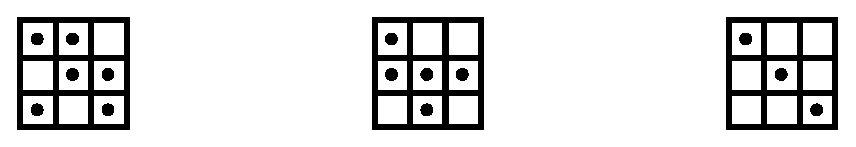
\includegraphics[scale=\s]{img/gridgame/gridgame1.pdf}\end{center}
\item There are two logical rules in this language.
The first rule is that if a particular proposition holds, then
its clockwise rotation by ninety degrees follows. So if 
\rb{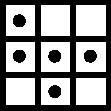
\includegraphics[scale=\s]{img/gridgame/gridgame2.pdf}}
holds, then you can deduce that
\rb{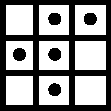
\includegraphics[scale=\s]{img/gridgame/gridgame3.pdf}}.
The second rule is that if two propositions $\pA$ and $\pB$ hold, then you can deduce a third proposition
which contains a dot in any square that has a dot in either $\pA$ or $\pB$, but not both.
So for example if you have the two propositions
\rb{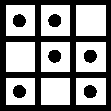
\includegraphics[scale=\s]{img/gridgame/gridgame6.pdf}}
and
\rb{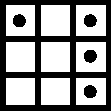
\includegraphics[scale=\s]{img/gridgame/gridgame7.pdf}},
then you can deduce from them that
\rb{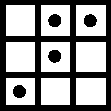
\includegraphics[scale=\s]{img/gridgame/gridgame5.pdf}}.
\item There are only two axioms in this language, and they are as follows:
\begin{center}
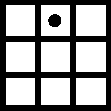
\includegraphics[scale=\s]{img/gridgame/gridgame8.pdf}
\hspace{2em}
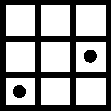
\includegraphics[scale=\s]{img/gridgame/gridgame9.pdf}
\end{center}
\end{itemize}
As a demonstration of this deductive language, here is a proof that 
\rb{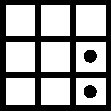
\includegraphics[scale=\s]{img/gridgame/gridgame11.pdf}}\ :
\begin{center}
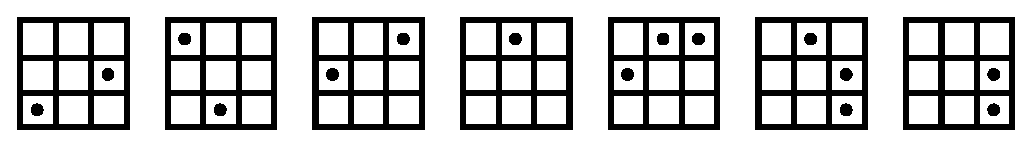
\includegraphics[scale=\s]{img/gridgame/gridgame10.pdf}
\end{center}
Can you see how this proof is correct?
These annotations may help:
\begin{center}
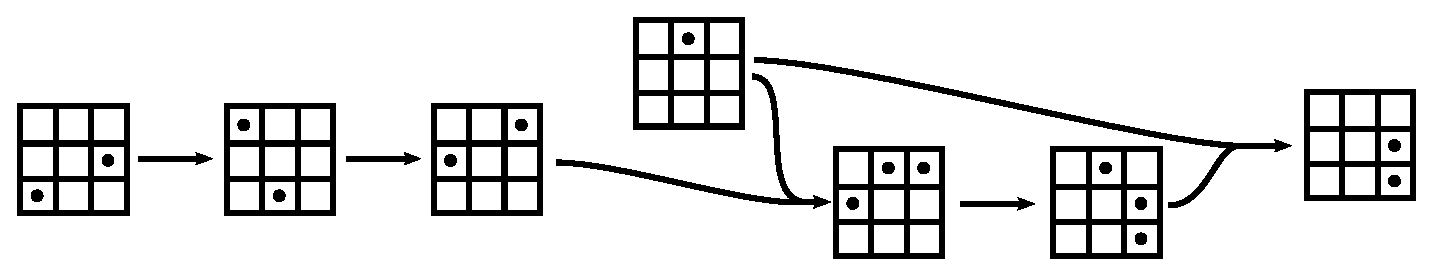
\includegraphics[scale=\s]{img/gridgame/gridgame12.pdf}
\end{center}
Now...
\begin{enumerate}
\item
How many propositions are there in this language?
How many propositions do you think there are in mathematics?
How many sentences are there in English?
\item
Give a completely formal proof that 
\rb{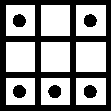
\includegraphics[scale=\s]{img/gridgame/gridgame0.pdf}}.
To help out your reader, annotate the proof with arrows like in the example above.
\item (Open-ended) Can you think of a way to write an \emph{informal} version of your proof?
It would be an English description of your proof that does not explain every detail but still captures the essence of your formal proof.
%One way to think of an informal proof is: it somehow gives the reader \emph{instructions} for how to come up with the formal proof.
\item (Irrelevant but fun) Can you figure out how many propositions in this language are provable and how many are not?
\end{enumerate}
}



\section{Logic and Writing Mathematical Arguments}
\label{sec:logic}

The rest of this course will introduce logic and set theory, starting with logic in this section.
Our goal with logic is not only to understand the rules of deduction,
but also to gain the ability to \emph{write} paragraph-style deductive arguments-- informal proofs.

Logic is all about manipulating \emph{propositions}, so you will not see many \emph{terms} showing up in this section.
In fact, we will find ourselves having to discuss proofs while having nothing in particular to prove anything about.
Mathematical propositions are supposed to say things about mathematical objects;
without any mathematical objects in hand, we cannot form any actual mathematical propositions.
We will proceed with the discussion anyway, using two strategies:

First, we will use the following capital Greek letters as placeholders for mathematical propositions:
$$
\pA,
\pB,
\pC,
\pD,
\pE,
\pF.
$$
When you see these capital Greek letters, remember that they are \emph{not variables},
at least not in the sense of mathematical variables. They are not to be replaced by mathematical \emph{objects}.
Rather, they are meant to be replaced by \emph{propositions}.
When they appear in English sentences, they will take the grammatical role of independent clauses.
So, for example, we accept the following as grammatically correct English sentences:
\begin{adjustwidth}{2em}{}
I believe that $\pA$.\\
They thought that $\pA$, but in fact $\pB$.\\
$\pA$.
\end{adjustwidth}

Our second strategy
%for discussing logic without the ability to form mathematical propositions 
is to apply the rules of logic to English sentences.
Even though $\pA$, $\pB$, etc. are supposed to stand for \emph{mathematical} propositions,
we will allow ourselves to replace them by declarative sentences in \emph{English}.
For example, replacing $\pA$ by ``Jim stole the car'' and $\pB$ by ``Jim is an upstanding guy'' in the above examples, we get the sentences
\begin{adjustwidth}{2em}{}
I believe that Jim stole the car.\\
They thought that Jim stole the car, but in fact Jim is an upstanding guy.\\
Jim stole the car.
\end{adjustwidth}
Later when we reach section
\ref{sec:sets}, we will start to work with actual mathematical propositions.

Section \ref{sec:logic_summary}
contains a reference table summarizing the logical constructions that are about to show up;
you can look there to get a sense for what is to come.

\ex{
Which of the following are grammatically correct? Hint: replace Greek letters with English sentences and see what makes sense.
\begin{enumerate}
\item She said that $\pC$, and I think she's onto something.
\item Take that, you accursed $\pA$!
\item Why don't we just $\pB$?
\item To $\pA$, or not to $\pA$, that is the question.
\item Whether $\pC$ or $\pD$, it will always be the case that $\pA$.
\item $\pD$ and $\pF$, but not $\pB$.
\item Despite all the $\pE$, they still wanted to $\pF$.
\item Whenever $\pC$, it turns out that $\pE$.
\item It is not true that $\pA$.
\end{enumerate}
}



\subsection{And, Or, and Not}

\paragraph{Conjunction}
\hypertarget{hl:AND}{Given} propositions $\pA$ and $\pB$, we can form their \emph{conjunction}
$$
\pA \AND \pB,
$$
which is expressed in English as ``$\pA$ and $\pB$.''
\hypertarget{hl:ANDUSE}{From} the conjunction $\pA\AND\pB$, you can deduce $\pA$ and you can deduce $\pB$.
\hypertarget{hl:ANDPV}{In} order to prove that $\pA\AND\pB$, you must prove both that $\pA$ and that $\pB$.
The following diagram, showing what you can deduce from $\pA\AND\pB$, kind of looks like the ``$\AND$'' symbol:
\begin{center}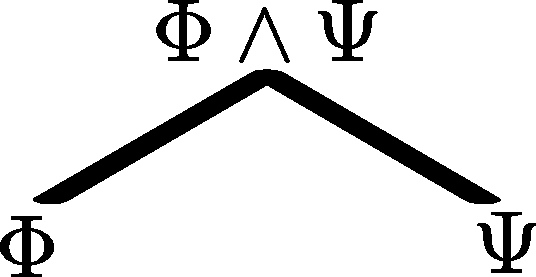
\includegraphics[scale=0.5]{img/andDiagram.pdf}\end{center}
Order does not matter for $\AND$; we consider $\pA\AND\pB$ and $\pB\AND\pA$ to be the same.


\paragraph{Disjunction}
\hypertarget{hl:OR}{Given} propositions $\pA$ and $\pB$, we can form their \emph{disjunction}
$$
\pA \OR \pB,
$$
which is expressed in English as ``$\pA$ or $\pB$.''
\hypertarget{hl:ORPV}{In} order to prove that $\pA\OR\pB$, you can either prove that $\pA$ or you can prove that $\pB$.
So if $\pA$ and $\pB$ happen to both hold, then you can still deduce that $\pA\OR\pB$
(unlike the way ``or'' is sometimes used in English).
The following diagram, showing what you can use to deduce $\pA\OR\pB$, kind of looks like the ``$\OR$'' symbol:
\begin{center}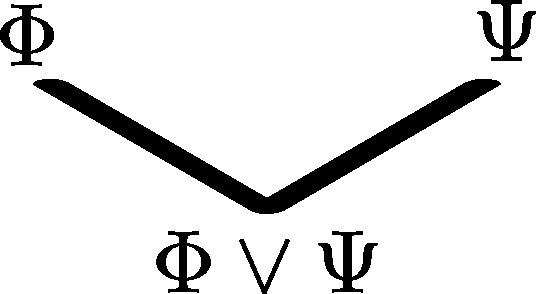
\includegraphics[scale=0.5]{img/orDiagram.pdf}\end{center}
Order does not matter for $\OR$; we consider $\pA\OR\pB$ and $\pB\OR\pA$ to be the same.

If you know that $\pA\OR\pB$, then how can you use this fact in your arguments?
You cannot deduce $\pA$ and you cannot deduce $\pB$, so how do you proceed if you want to prove some other proposition $\pC$?
\hypertarget{hl:ORUSE}{The} rule that lets you proceed is called \emph{proof by cases}:
\RULE{Proof by cases}{
Suppose that you can prove $\pC$ by assuming $\pA$, and you can also prove $\pC$ by assuming $\pB$.
Then you can deduce $\pC$ from $\pA\OR\pB$.
}
In a written proof, the format of a proof by cases ends up like this:

\THMMOCK{Assuming that either $\pA$ or $\pB$ holds, we have $\pC$.}{
Assume that either $\pA$ or $\pB$ holds.\\
Case 1: Suppose that $\pA$ holds.
\indented{[insert argument here convincing the reader that $\pC$ holds]}
Case 2: Suppose that $\pB$ holds.
\indented{[insert argument here convincing the reader that $\pC$ holds]}
Since $\pC$ holds in both cases, we can conclude that $\pC$ holds.
}

Let's do an example using English sentences.
Say you are hiking with your friend, and you see your friend brush past a plant with three-leaf bunches. You're not sure if it's poison ivy or poison oak, but you
know that it is one of them, and you know that both plants will cause a rash when touched.
So you argue to your friend: ``Suppose that plant was poison ivy. Then you would get a rash.
Now suppose the plant was poison oak. Then you would also get a rash. I'm sure that the plant was either poison ivy or it was poison oak, so you can expect a rash my friend.''
%Suppose you see a plant with three-leaf bunches and you're sure that it's either poison ivy or poison oak, but you don't know which.
%Well, you do know that poison ivy is poisonous and that poison oak is poisonous, so you can at least conclude that the plant you see is poisonous, even
%if you don't know which type of plant it is.
That's a proof by cases.
To make the proof structure apparent in
the formatting given above, replace $\pA$ by ``the plant is poison ivy,'' replace $\pB$ by ``the plant is poison oak,'' and replace $\pC$ by ``you will get a rash.''

%You get something like this:
%\THM{Assuming that the plant is either poison ivy or poison oak, we can conclude that it is poisonous.}{
%Assume that the plant is either poison ivy or poison oak.\\
%Case 1: Suppose the plant is poison ivy.
%\indented{[insert argument convincing the reader that poison ivy is poisonous.]}
%Case 2: Suppose the plant is poison oak.
%\indented{[insert argument convincing the reader that poison oak is poisonous.]}
%Since the plant is poisonous either way, we can conclude that the plant is poisonous.
%}

\paragraph{Negation}
\hypertarget{hl:NOT}{Given} a proposition $\pA$, we can form its \emph{negation}
$$
\neg \pA,
$$
which is expressed in English as ``it is not the case that $\pA$.''
To prove $\neg\pA$ is to disprove $\pA$, and in fact this is what ``disprove'' means.
When $\pA$ holds we say that $\pA$ is \emph{true}, and when $\neg\pA$ holds we say that $\pA$ is \emph{false}.
We consider $\neg\neg\pA$ to be the same as $\pA$.

%It should never be the case that a proposition holds while its negation also holds.
%We hope, at least, that $\pA\AND\not\PA$ is not provable.
A proposition of the form $\pA\AND\neg\pA$ is called a \emph{contradiction}.
If something can both be and not be the case, then our entire deductive system is certainly broken.
We hope that no contradiction is provable in our language.
\hypertarget{hl:NOTPV}{This} leads us to accept the following as a way of proving a negation $\neg\pA$:
%Further, we explicitly deem contradictions to be \emph{impossible}, in the sense that any assumption
%that leads one to deduce a contradiction must be rejected as false.
%In order to prove that $\neg\pA$, you can assume that $\pA$ does hold and then show that this leads to a contradiction.
%This is called a \emph{proof by contradiction}:
\RULE{Proof by contradiction}{
If assuming $\pA$ allows you to deduce a contradiction, then it must be that $\neg\pA$.
}
In a written proof, the format of a proof by contradiction ends up like this:

\THMMOCK{$\neg\pA$.}{
Suppose, for the sake of obtaining a contradiction, that $\pA$ holds.
\indented{[insert argument convincing reader that a contradiction, something of the form $\pB\AND\neg\pB$, now follows]}
Since this is a contradiction, we conclude that $\neg\pA$.
}

Let's do an example using English sentences.
Say you're investigating a crime and you are considering a particular suspect.
Assuming the suspect did commit the crime, you can deduce that the suspect must have been at the crime scene on that day.
Upon questioning witnesses, you discover that the suspect was at work and could not have been at the crime scene that day.
This contradiction leads you to reject the original assumption; the suspect must not have committed the crime.
Making an assumption so that you can reject it after deducing an impossible situation-- that is a proof by contradiction.
To make the proof structure apparent in
the formatting given above, replace
$\pA$ by ``the suspect committed the crime'' and replace $\pB$ by ``the suspect was at the crime scene that day''.


The proof by contradiction rule rejects that a mathematical proposition can be both true and false.
There's
another rule involving negation which
enforces that mathematical propositions must be either true or false:
\RULE{Excluded middle}{
$\pA\OR\neg\pA$
}
There is no ``middle ground'' in which a proposition is neither true nor false.






% go back and do a better job presenting rules in terms of  formatting, and separatign susbsections perhaps with illustrated titles



% exercise that helps to understand how in english you can have inclusive and exclusive or, while math is inclusive.

% exercise that shows how parentheses are needed in and-or combinations
% in the same exercise you can show how and distributes over or and vice versa
% maybe the ex can be structured like this: for each of the following deductions, decide whether it is valid or not. if not valid, then justify by... 
  % uhhh truth table? or maybe you can give them some sample true and false english facts to put in, and do an example.

% some kind of exercise involving demorgan's law. or maybe you should write about that above
% idea: a deduction of demorgan's law going one way, and have them prove it going the other way

% maybe an exercise involving truth tables, having them fill one out for basic things and then for more complicated props

\ex{
The ``or'' of mathematical logic sometimes behaves differently from the English ``or.''
Describe a situation in which
\begin{center} ``The cake is flavored with either vanilla or chocolate.'' \end{center}
would pretty much be considered false, while
\begin{center} ``The cake is flavored with vanilla''\ $\OR$\ ``The cake is flavored with chocolate''. \end{center}
would be true.
}


\ex{
Suppose we know the following three facts:
\begin{itemize}
\item Whenever it rains over night, the grass gets wet. 
\item On a night that it doesn't rain, the sprinklers are run.
\item Whenever sprinklers are run, the grass gets wet.
\end{itemize}
Now write a proof of the following statement: ``The grass got wet last night.''
To make your argument, apply excluded middle to the statement ``It rained last night,''
and then do a proof by cases.
Follow the formatting given in this section for proof by cases.
}


\ex{
Suppose we know the following four facts:
\begin{itemize}
\item Whenever it rains over night, the grass gets wet. 
\item On a night that it doesn't rain, the sprinklers are run.
\item Whenever sprinklers are run, \emph{as long as they are not broken}, the grass gets wet.
\item The grass was dry last night.
\end{itemize}
Now write a proof of the following statement: ``It did not rain last night and the sprinklers are broken.''
To make your argument,
do a proof by contradiction to establish ``it did not rain last night,''
and do another proof by contradiction to establish ``the sprinklers are broken.''
Once both are established you can conclude the conjunction.
Follow the formatting given in this section for proof by contradiction.
}





\newcommand{\truthtablefour}[5]{
\begin{tabular}{|c|c|c|}
\hline
$\pA$ & $\pB$ & #1 \\ \hline
F     & F  & #2   \\ \hline
F     & T  & #3   \\ \hline
T     & F  & #4   \\ \hline
T     & T  & #5   \\ \hline
\end{tabular}
}

\newcommand{\truthtabletwo}[3]{
\begin{tabular}{|c|c|}
\hline
$\pA$ & #1 \\ \hline
F     & #2   \\ \hline
T     & #3   \\ \hline
\end{tabular}
}


\def\sp{\hspace{1em}}

\ex{
Thanks to the law of excluded middle, there are only two possibilities for a single proposition $\pA$: it is either true or false.
For \emph{two} propositions $\pA$ and $\pB$, there are \emph{four} possibilities, which we can list in a nice table:
\begin{center}
\begin{tabular}{|c|c|}
\hline
$\pA$ & $\pB$ \\ \hline
F     & F     \\ \hline
F     & T     \\ \hline
T     & F     \\ \hline
T     & T     \\ \hline
\end{tabular}
\end{center}
For three propositions there are eight possibilities, and so on.
This suggests a useful way to think about the logical operators $\AND$, $\OR$, and $\neg$:
\begin{center}
\truthtablefour{$\pA\AND\pB$}{F}{F}{F}{T}
\sp
\truthtablefour{$\pA\OR\pB$}{F}{T}{T}{T}
\sp
\truthtabletwo{$\neg\pA$}{T}{F}
\end{center}
Here we are simply listing all the possibilities for the component propositions $\pA$, $\pB$, etc.,
and then we are indicating whether the complex proposition is true or false in each case. These are called \emph{truth tables}.
\begin{enumerate}
\item
Write out a truth table for $\neg(\pA\AND\pB)$. It should have four rows.

\item
Write out a truth table for $(\pA\AND\pB)\OR\pC$, and also for $\pA\AND(\pB\OR\pC)$.
The table should have eight rows, and you can feel free to make just one table in which 
there is a column for $(\pA\AND\pB)\OR\pC$ and a column for $\pA\AND(\pB\OR\pC)$.

\item
Your answer to the above should convince you that it's a terrible idea to write something like ``$\pA\AND\pB\OR\pC$.''
Replace $\pA$, $\pB$, and $\pC$ by English sentences in $\pA\AND\pB\OR\pC$ such that you get an ambiguous English sentence.
Explain the ambiguity in your sentence.

\item \label{itm:truthtables:first_equiv}
Write out a truth table for $(\pA\AND\pB)\AND\pC$, and also for $\pA\AND(\pB\AND\pC)$.
The answer should convince you that there is no trouble at all with writing $\pA\AND\pB\AND\pC$,
though you were probably convinced anyway since $\pA\AND\pB\AND\pC$ can obviously only mean:
``$\pA$, $\pB$, and $\pC$ are all true.''

\item
Write out a truth table for $(\pA\AND\pB)\OR\pA$. This one should just have four rows.
Looking at the table, do you see a way to ``simplify'' the complex proposition  $(\pA\AND\pB)\OR\pA$?

\item
Write out a truth table for $(\pA\AND\pB)\OR\pC$, and also for $(\pA\OR\pC)\AND(\pB\OR\pC)$.
This should show you that $\OR$ can ``distribute'' over $\AND$.

\item
Write out a truth table for $(\pA\OR\pB)\AND\pC$, and also for $(\pA\AND\pC)\OR(\pB\AND\pC)$.
This should show you that $\AND$ can ``distribute'' over $\OR$.

\item \label{itm:truthtables:last_equiv}
Write out a truth table for $\neg(\pA\AND\pB)$, and also for $(\neg\pA)\OR(\neg\pB)$.
\end{enumerate}
In parts \ref{itm:truthtables:first_equiv} through \ref{itm:truthtables:last_equiv},
you see that certain propositions are ``equivalent'' in some sense. The formal meaning of ``equivalent'' will be
discussed in the next section.
}


\subsection{If and Iff}

\paragraph{Implication}
\hypertarget{hl:ARR}{Given} propositions $\pA$ and $\pB$, we can form the \emph{implication}
$$
\pA\ARR\pB,
$$
which is expressed in English as ``$\pA$ implies $\pB$'' or ``if $\pA$, then $\pB$.''
The ``$\pA$'' part of an implication $\pA\ARR\pB$ is called the \emph{hypothesis},
and the ``$\pB$'' part is called the \emph{conclusion}.
\hypertarget{hl:ARRPV}{To} prove $\pA\ARR\pB$,
start by assuming $\pA$ and
then give an argument that $\pB$ follows.
That is, assume the hypotheses and then argue that the conclusion follows.
Such a proof ends up structured like this:

\THMMOCK{If $\pA$, then $\pB$.}{
Assume that $\pA$.
\indented{[insert argument convincing reader that $\pB$ holds]}
Thus, $\pA\ARR\pB$.
}

\hypertarget{hl:ARRUSE}{The} rule that allows us to use $\pA\ARR\pB$ is modus ponens:
\RULE{Modus Ponens\label{rule:mp}}{
Given $\pA\ARR\pB$ and $\pA$, you can deduce $\pB$.
}
Here is also another great rule for using an implication (this one can be derived from modus ponens via a proof by contradiction):
\DRULE{Modus Tollens}{
Given $\pA\ARR\pB$ and $\neg\pB$, you can deduce $\neg\pA$.
}

\paragraph{Logical Equivalence}
\hypertarget{hl:DARR}{Given}  propositions $\pA$ and $\pB$, we can form the \emph{logical equivalence}
$$
\pA\DARR\pB,
$$
which is expressed in English as ``$\pA$ if and only if $\pB$,'' often shortened to ``$\pA$ iff $\pB$.''

An equivalence holds when two propositions are forced to be true or false \emph{together}--
that is, when they are either both true or both false.

\hypertarget{hl:DARRPV}{To} prove an equivalence $\pA\DARR\pB$, simply prove both of the implications $\pA\ARR\pB$ and $\pB\ARR\pA$.
The proof will be structured like this:

\THMMOCK{$\pA\DARR\pB$.}{
Assume that $\pA$.
\indented{[insert argument convincing reader that $\pB$ holds]}
Now assume that $\pB$.
\indented{[insert argument convincing reader that $\pA$ holds]}
}

\hypertarget{hl:DARRUSE}{Using} an equivalence works a lot like modus ponens, except it goes in both directions.
If you know that $\pA\DARR\pB$, then you can deduce $\pA$ from $\pB$, $\neg\pA$ from $\neg\pB$,
$\pB$ from $\pA$, and $\neg\pB$ from $\neg\pA$.



\def\sp{\hspace{1em}}

Here are the truth tables for $\ARR$ and $\DARR$:
\begin{center}
\truthtablefour{$\pA\ARR\pB$}{???}{???}{F}{T}
\sp
\truthtablefour{$\pA\DARR\pB$}{T}{F}{F}{T}
\end{center}
There should be nothing surprising there, except that I've left some question marks in position where I think you might be surprised.
If $\pA$ is false, then what of the proposition $\pA\ARR\pB$?
It has to be either true or false (due to excluded middle), so which is it?
Put another way: Suppose you say ``If $3$ is even, then $3$ is divisible by $2$.''
Knowing that $3$ is not even, are you a liar? Is your statement true or false?
The answer is that it's \emph{true}!
Here is the completed truth table for $\ARR$:
\begin{center}
\truthtablefour{$\pA\ARR\pB$}{T}{T}{F}{T}
\end{center}
\hypertarget{hl:vacuous}{Putting} T there is not an arbitrary choice-- if you agreed with all the previous logical rules then you \emph{must} agree
that $\pA\ARR\pB$ is \emph{true} when $\pA$ is false.
Let me try and convince you. First we need to revisit contradictions.


\def\vsp{\\[0.5em]}

Recall how \emph{proof by contradiction} works:
If an assumption leads to a contradiction, then the assumption is rejected as false.
If you assume $\pB$, and then after some argumentation you deduce $\pA\AND\neg\pA$, then
you can back out of your original assumption and conclude without a doubt that $\neg\pB$.
Now let's think, hypothetically, what would happen if a contradiction $\pA\AND\neg\pA$ were actually \emph{true}?
If $\pA\AND\neg\pA$ holds, then we can prove $\pB$ by contradiction as follows:
\indented{
Suppose, for the sake of contradiction, that $\neg\pB$ holds.\vsp
Since $\pA\AND\neg\pA$ has already been assumed to hold, we've already reached a contradiction.\vsp
We conclude that $\neg\neg\pB$, and therefore $\pB$, must hold.
}
Let's be clear about what just happened: from the assumption $\pA\AND\neg\pA$, we were able to prove an \emph{arbitrary proposition}!
This mechanism was always present in the proof by contradiction rule, but it is worth highlighting:

\DRULE{\label{rule:contradictions}Contradictions are powerful!}{
From $\pA\AND\neg\pA$ you can deduce \emph{any} proposition $\pB$.
}

Now back to the question of how to treat $\pA\ARR\pB$ when $\pA$ is false.
Recall that in order to prove $\pA\ARR\pB$, one can assume $\pA$ and then deduce $\pB$.
If we know that $\pA$ is false to start with, then here is a proof that $\pA\ARR\pB$:
\indented{
Assume $\pA$.\vsp
Since $\pA$ is known to be false, we now have a contradiction $\pA\AND\neg\pA$.\vsp
Using ``contradictions are powerful,'' we can now deduce anything we want! In particular, we can deduce $\pB$.
}
Thus if you accept proofs by contradiction as valid, then you must accept that $\pA\ARR\pB$ is true when $\pA$ is false.
An implication that is true because its hypothesis is false is sometimes said to be \emph{vacuously true}.

\ex{
Assume that we know the following facts:
\begin{itemize}
\item Alice is an accountant and holds no other profession.
\item Bob has brown hair.
\item Charles loves chocolate and despises all other foods.
\end{itemize}
Determine whether each of the following is true or false.
\begin{enumerate}


\item %3
If
Bob's hair is purple
then
Charles loves chocolate.


\item %2
If
Alice is an accountant
then
Charles likes green beans.


\item %6
Alice is an accountant
if and only if
Alice is a doctor.


\item %1
If
Bob has brown hair
then
Charles loves chocolate.


\item %7
Charles likes baked salmon
if and only if
Bob has brown hair.


\item %8
Charles likes clam chowder
if and only if
Alice is a professional underwater welder.

\item %4
If
Bob's hair is green
then
Bob's hair is white.

\item %5
Bob's hair is brown
if and only if
Charles loves chocolate.


\end{enumerate}

Notice how the implication of mathematical logic has nothing to do with causality.
Some of the sentences above sound weird in English because we often use ``if... then...'' to 
indicate that one state of affairs \emph{causes} another, as in the sentence
\begin{center}``If you don't brush your teeth, then you will get cavities.''\end{center}
In mathematical logic, that sentence is simply true if you either brush your teeth, or if you don't brush your teeth and end up getting cavities.
Interestingly, that sentence is true even in a situation where you brush your teeth and still get cavities.
That's quite different from the ``if... then...'' of conversational English!
In conversation, we would expect there to be an implicit
\begin{center}``(And if you do brush your teeth then you will not get cavities.)''\end{center}
Be aware that this implicit additional statement is not there in mathematical logic; 
an implication $\pA\ARR\pB$ doesn't give you any information in the case where you know that $\neg\pA$.
}

\ex{
Write a truth table for $(\pA\ARR\pC)\AND(\pB\ARR\pC)$. It should have eight rows.
In the same truth table, add a column for $(\pA\OR\pB)\ARR\pC$.
Finally, in the same truth table, add a column for 
$$((\pA\ARR\pC)\AND(\pB\ARR\pC))\ARR((\pA\OR\pB)\ARR\pC).$$
The latter proposition could be called ``proof by cases,'' and so your truth table result should not be too surprising.
}

\subsection{Some Derived Logical Rules}
\label{sec:derived1}

In this section we will derive some logical rules from the basic ones given in previous sections.
We still have no specific mathematical propositions to talk about and so we still use the placeholders $\pA$, $\pB$, etc.
The arguments given in this section are useful logical patterns that can help us build other arguments later on.

The following derived rule could be written as ``$((\pA\ARR\pB)\AND(\pB\ARR\pC))\ARR(\pA\ARR\pC)$'',
but we instead mix in some English to cut down on the number of parentheses and to make things more pleasant to read.

\DRULEPF{Transitivity of Implication\label{DRULE:trans_impl}}{
If $\pA\ARR\pB$ and $\pB\ARR\pC$, then $\pA\ARR\pC$.
}{
Assume that $\pA\ARR\pB$ and $\pB\ARR\pC$.
In order to prove that $\pA\ARR\pC$, let us assume $\pA$.
(Our goal is now to prove $\pC$.)
From $\pA$ and $\pA\ARR\pB$, it follows that $\pB$.
From $\pB$ and $\pB\ARR\pC$, it follows that $\pC$.
}

In the above argument you can see two applications of modus ponens-- this is how implications can be put to use.
And you can also see how an implication is proven, by assuming the hypotheses and arguing for the conclusion.

\def\lsp{\\[-0.4em]}

\DRULEPF{Conjunction and Implication}{
$(\pA\AND\pB)\ARR\pC$ if and only if $(\pA\ARR(\pB\ARR\pC))$
}{
Assume that $(\pA\AND\pB)\ARR\pC$.
In order to prove $(\pA\ARR(\pB\ARR\pC))$, assume $\pA$.
Now in order to prove $\pB\ARR\pC$, assume $\pB$.
Since we have both $\pA$ and $\pB$, we have $\pA\AND\pB$.
Since $(\pA\AND\pB)\ARR\pC$, we can now conclude $\pC$.\lsp

Now assume that $(\pA\ARR(\pB\ARR\pC))$.
In order to prove that $(\pA\AND\pB)\ARR\pC$,
assume $\pA\AND\pB$.
That is, we have assumed $\pA$ and we have assumed $\pB$.
From $\pA$ and $\pA\ARR(\pB\ARR\pC)$, it follows that $\pB\ARR\pC$.
From $\pB$ and $\pB\ARR\pC$, it follows that $\pC$.
}

The first thing to notice about the above argument is the way in which an ``if and only if'' statement gets proven.
There are two parts to the proof, one for each of the two implications.
The first half of the proof establishes 
$$((\pA\AND\pB)\ARR\pC)\ARR((\pA\ARR(\pB\ARR\pC))),$$
while the second half establishes
$$((\pA\ARR(\pB\ARR\pC)))\ARR((\pA\AND\pB)\ARR\pC).$$
Together, they allow us to conclude the ``if and only if'' statement
$$((\pA\AND\pB)\ARR\pC)\DARR((\pA\ARR(\pB\ARR\pC))).$$
Another thing to notice is the way in which $\AND$ is handled.
In the first half of the argument, we establish that $\pA\AND\pB$ holds by establishing each of $\pA$ and $\pB$-- this is the way to prove a conjunction.
In the second half, we get to assume that $\pA\AND\pB$ holds and this allows us to deduce both $\pA$ and $\pB$-- this is the way conjunctions get used.
In typical proofs this handling of conjunctions happens very quickly; the distinction between
\begin{center} ``Assume that $\pA\AND\pB$''\end{center}
and
\begin{center} ``Assume that $\pA$ and assume that $\pB$''\end{center}
will be blurred completely.

\DRULEPZ{}{If $\pA\ARR\pB$ and $\pC\ARR\pD$, then $(\pA\AND\pC)\ARR(\pB\AND\pD)$.}

\DRULEPF{Disjunction and Implication}{
$(\pA\OR\pB)\ARR\pC$ if and only if $(\pA\ARR\pC)\AND(\pB\ARR\pC)$
}{
$\Rightarrow$:
Assume that $(\pA\OR\pB)\ARR\pC$.
\lsp

In order to prove that $(\pA\ARR\pC)$, assume $\pA$.
From $\pA$ it follows that $\pA\OR\pB$.
From $\pA\OR\pB$ and $(\pA\OR\pB)\ARR\pC$, we can conclude that $\pC$.
Thus we have proven that $\pA\ARR\pC$.
\lsp

We also need to prove that $\pB\ARR\pC$. To this end, assume $\pB$.
From $\pB$ it follows that $\pA\OR\pB$.
From $\pA\OR\pB$ and $(\pA\OR\pB)\ARR\pC$, we can conclude that $\pC$.
Thus we have proven that $\pB\ARR\pC$.
\lsp

Since we proved $\pA\ARR\pC$ and $\pB\ARR\pC$, we can conclude that $(\pA\ARR\pC)\AND(\pB\ARR\pC)$.
\lsp

$\Leftarrow$: 
Assume that $(\pA\ARR\pC)\AND(\pB\ARR\pC)$.
That is, assume  $\pA\ARR\pC$ and assume $\pB\ARR\pC$.
For the sake of proving $(\pA\OR\pB)\ARR\pC$, assume that $\pA\OR\pB$.
\lsp

Case 1: In the case that $\pA$ holds, it follows from $\pA\ARR\pC$ that $\pC$ holds.
\lsp

Case 2: In the case that $\pB$ holds, it follows from $\pB\ARR\pC$ that $\pC$ holds.
\lsp

Since $\pC$ holds in both cases, we conclude that $\pC$ holds.
}

Here the two halves of the ``if and only if'' proof are difficult to separate by paragraphs alone, since each half needed multiple paragraphs.
So the two halves of the proof are headed by ``$\Rightarrow$'' and ``$\Leftarrow$''.
You should always feel free to use headings to separate different components of your argument.

Another thing to notice in the above argument is the way in which $\OR$ is handled.
In the first half of the argument, we establish $\pA\OR\pB$ by deducing it from $\pA$, and we also establish it by deducing it from $\pB$.
In the second half, we use an $\OR$ statement in pretty much the only way we can-- a proof by cases.

\DRULEPZ{}{If $\pA\ARR\pB$ and $\pC\ARR\pD$, then $(\pA\OR\pC)\ARR(\pB\OR\pD)$.}

\DRULEPF{Alternative Eliminated\label{DRULE:alt_elim}}{
If $\pA\OR\pB$ holds but $\pA$ does not hold, then $\pB$ must hold.
In other words,
$$((\pA\OR\pB)\AND(\neg\pA))\ARR\pB.$$
}{
Assume that $\pA\OR\pB$ holds and $\neg\pA$ holds.
\lsp

Case 1: Suppose that $\pA$ holds.
Then we have $\pA\AND\neg\pA$! From a contradiction we can conclude anything, in particular we can conclude that $\pB$ holds.
\lsp

Case 2: Suppose that $\pB$ holds... that's it for case 2.
\lsp

In both cases we conclude $\pB$, so we can conclude $\pB$.
}

In the above argument we've made use of rule \ref{rule:contradictions}.


\DRULEPF{Or Distributes over And}{
$(\pA\OR(\pB\AND\pC))\DARR((\pA\OR\pB)\AND(\pA\OR\pC))$.
}{
$\Rightarrow$:
Assume $\pA\OR(\pB\AND\pC)$.
\lsp

Case 1: Suppose $\pA$ holds. Then we can immediately conclude $\pA\OR\pB$ and $\pA\OR\pC$, and from these
we can conclude $(\pA\OR\pB)\AND(\pA\OR\pC)$.
\lsp

Case 2: Suppose $\pB\AND\pC$ holds.
Then $\pB$ holds, and $\pA\OR\pB$ then follows from that.
Also $\pC$ holds, and $\pA\OR\pC$ follows from that.
Finally we conclude $(\pA\OR\pB)\AND(\pA\OR\pC)$.
\lsp

Since both cases lead to $(\pA\OR\pB)\AND(\pA\OR\pC)$, we conclude $(\pA\OR\pB)\AND(\pA\OR\pC)$.
\lsp

$\Leftarrow$: Assume $((\pA\OR\pB)\AND(\pA\OR\pC))$.
That is, assume $\pA\OR\pB$ and assume $\pA\OR\pC$.
Due to excluded middle, we know that either $\pA$ or $\neg\pA$ holds.
\lsp

Case 1: Suppose that $\pA$ holds. It immediately follows that $\pA\OR(\pB\AND\pC)$.
\lsp

Case 2: Suppose that $\neg\pA$ holds. Using the rule ``alternative eliminated,''
it then follows from $\pA\OR\pB$ that $\pB$ holds.
Similarly, it follows from $\pA\OR\pC$ that $\pC$ holds. Thus $\pB\AND\pC$ holds.
Finally, we conclude that $\pA\OR(\pB\AND\pC)$.
\lsp

Since both cases lead to $\pA\OR(\pB\AND\pC)$, we conclude $\pA\OR(\pB\AND\pC)$.
}

Observe that a proof by cases need not proceed from the exact $\OR$-proposition one has assumed;
sometimes it is useful to do a proof by cases based on excluded middle.

%\DRULEPZ{And Distributes over Or}{
%$(\pA\AND(\pB\OR\pC))\DARR((\pA\AND\pB)\OR(\pA\AND\pC))$.
%}
%
%The following rule was actually already used in an argument in the previous section.
%It's interesting to see that this rule can be derived from prior rules.
%
%\DRULEPF{Double Negation}{
%$\pA\DARR(\neg\neg\pA)$.
%}{
%Assume $\pA$. Assume, for the sake of obtaining a contradiction, that $\neg\pA$.
%Then we immediately have a contradiction $\pA\AND\neg\pA$, and so we conclude that $\neg\neg\pA$.
%\lsp
%
%Now assume $\neg\neg\pA$.
%Our goal is to prove $\pA$.
%Due to excluded middle, we have that $\pA\OR\neg\pA$.
%In the case that $\pA$ holds, we are done with the proof. 
%In the case that $\neg\pA$ holds, we have the contradiction 

%% THIS IS CIRCULAR! The problem is that Contradictions are Powerful was supposed to be an axiom, and I'm using proof by contradiction as an axiom instead.
%% Proof by contradiction only allows you to prove negations.

%}








% Define notions of converse, inverse, and contrapositive.
Given an implication $\pA\ARR\pB$, there are a few ``flipped'' implications one can write down:
\indented{The \emph{converse} of $\pA\ARR\pB$ is $\pB\ARR\pA$.\\
          The \emph{inverse} of $\pA\ARR\pB$ is $\neg\pA\ARR\neg\pB$.\\
          The \emph{contrapositive} of $\pA\ARR\pB$ is $\neg\pB\ARR\neg\pA$.}
It is a common mistake to think that the converse or the inverse of an implication follows from the implication.
The confusion stems from the inconsistent ways in which ``if... then...'' can work in conversation.
When a bank robber says
\begin{center}
``If you don't hand over the money, I'll shoot!'',
\end{center}
they implicitly also mean to say the inverse
\begin{center}
``If you do hand over the money, then I won't shoot!'',
\end{center}
and the converse
\begin{center}
``I'll shoot only if you don't hand over the money!''
\end{center}
If the bank robber were using strict mathematical logic (that is, if their original
threat took the form ``you don't hand over the money''$\ARR$``I will shoot''), then
they could, without lying, shoot even after the money is handed over.

The \emph{contrapositive} of an implication, on the other hand, \emph{does} follow from the implication.
This rule is derived below.
\hypertarget{hl:contraposition}{An} implication is always equivalent to its contrapositive.
Since the converse of an implication is the contrapositive of its inverse, the converse and inverse of an implication are equivalent.






% Prove that impliation holds iff contrapositive does.
\DRULEPF{Contraposition\label{drule:contraposition}}{$(\pA\ARR\pB)\DARR(\neg\pB\ARR\neg\pA)$}{
Assume that $\pA\ARR\pB$.
To prove that $\neg\pB\ARR\neg\pA$, assume that $\neg\pB$.
Now assume $\pA$, for the sake of obtaining a contradiction.
Since $\pA\ARR\pB$, we see that $\pB$ follows. We end up with the contradiction $\pB\AND\neg\pB$.
Thus we reject the original assumption and conclude that $\neg\pA$.
\lsp

Now to prove the other direction, assume that $\neg\pB\ARR\neg\pA$.
To prove that $\pA\ARR\pB$, assume $\pA$.
For the sake of obtaining a contradiction, assume $\neg\pB$.
From $\neg\pB\ARR\neg\pA$, it then follows that $\neg\pA$.
But we've now reached the contradiction $\pA\AND\neg\pA$.
Thus we reject the original assumption and conclude that $\neg\neg\pB$.
In other words, $\pB$.
}

% Comment on how pf by contradiction appears as a great tool for disproving something.
The above argument is a great demonstration of how proofs by contradiction work.
Sometimes, in order to proceed with your argument, you need something \emph{more} to work with.
Assuming that your desired conclusion doesn't hold can sometimes give you something more and help push your argument forward.

The above argument should make you feel that ``proof by contradiction'' and ``contraposition'' are very closely related.
%The theorems you prove will most often take the form of an implication, something like
%\begin{center}If $\pA$, $\pB$, and $\pC$, then $\pD$. \end{center}
One can prove $\pA\ARR\pB$ by assuming $\pA$, then assuming $\neg\pB$ and trying to obtain a contradiction.
Or, one can prove $\pA\ARR\pB$ by instead proving its contrapositive $\neg\pB\ARR\neg\pA$, which we now see is equivalent to the original implication.
Both approaches amount to pretty much the same argument.

\vspace{1em}

\DRULEPF{\hypertarget{hl:invertEquiv}{Inverting} an Equivalence\label{drule:neg_equiv}}{
If $\pA\DARR\pB$, then $\neg\pA\DARR\neg\pB$.
}{
Assume that $\pA\DARR\pB$. Then $\pA\ARR\pB$ and $\pB\ARR\pA$.
By contraposition, it follows that $\neg\pB\ARR\neg\pA$ and $\neg\pA\ARR\neg\pB$.
Thus we have $\neg\pA\DARR\neg\pB$.
}

% do LXXXIII ii
\DRULEPF{De Morgan's Law 1\label{drule:demorgan1}}{$\neg(\pA\AND\pB)\ \DARR\ (\neg\pA\OR\neg\pB)$}{
$\Rightarrow$: Assume $\neg(\pA\AND\pB)$.
Due to excluded middle, either $\pA$ or $\neg\pA$.\lsp

Case 1: Suppose that $\pA$ holds. Now if $\pB$ held we would obtain $\pA\AND\pB$, which leads to the contradiction $(\pA\AND\pB)\AND\neg(\pA\AND\pB)$.
Therefore it must be that $\neg\pB$. From this it follows that $\neg\pA\OR\neg\pB$.\lsp

Case 2: Suppose that $\neg\pA$ holds. Then it immediately follows that $\neg\pA\OR\neg\pB$.\lsp

Since we ended up with $\neg\pA\OR\neg\pB$ in both cases, we can conclude that $\neg\pA\OR\neg\pB$.
\\[1em]

$\Leftarrow$: Assume $(\neg\pA)\OR(\neg\pB)$.
Suppose, for the sake of contradiction, that $\pA\AND\pB$ holds.
Then $\pA$ holds, and $\pB$ holds. Since we know that $(\neg\pA)\OR(\neg\pB)$ holds, there are two cases to consider:\lsp

Case 1: Suppose that $\neg\pA$ holds. Then, since we already said that $\pA$ holds, we obtain the contradiction $\pA\AND\neg\pA$.\lsp

Case 2: Suppose that $\neg\pB$ holds. Then, since we already said that $\pB$ holds, we obtain the contradiction $\pB\AND\neg\pB$.\lsp

We obtain a contradiction either way, and so we are forced to reject that $\pA\AND\pB$. That is, we have $\neg(\pA\AND\pB)$.
}



% puzzle LXXXIII i
\DRULEPZ{De Morgan's Law 2\label{drule:demorgan2}}{
$\neg(\pA\OR\pB)\ \DARR\ (\neg\pA\AND\neg\pB)$
}


% do LXXXVII i but make the forward direction a puzzle, with hint to use excluded middle
\DRULEPF{Implication in Terms of Disjunction\label{drule:unless}}{
$(\pA\ARR\pB)\DARR(\neg\pA\OR\pB)$
}{
$\Rightarrow$: \putExerciseHeading: Prove that $(\pA\ARR\pB)\ARR(\neg\pA\OR\pB)$. Hint: Use excluded middle.
\lsp

$\Leftarrow$: Assume that $\neg\pA\OR\pB$. With the goal of proving that $\pA\ARR\pB$, assume that $\pA$.
Applying the previous rule ``alternative eliminated,''
we can conclude $\pB$ from $\neg\pA\OR\pB$ and $\pA$.
}

% comment on the inutiitiveness of this as ``$\pB$, unless $\neg\pA$'', and on how it means implications were not needed
The fact that $\pA\ARR\pB$ can be rewritten as $\neg\pA\OR\pB$ suggests that we never needed to formally introduce $\ARR$ into our language.
Every time we want to say ``if $\pA$, then $\pB$,'' we could instead say ``either $\pB$, or it's not the case that $\pA$.''
But life is better when we can phrase things in terms of $\ARR$, and that is why we choose to have it.

% puzzle $\neg(\pA\ARR\pB)\DARR (\pA\AND\neg\pB)$
\DRULEPZ{Negating an Implication\label{drule:neg_impl}}{$\neg(\pA\ARR\pB)\DARR (\pA\AND\neg\pB)$}

% comment that it's important to understand this so that we know how to negate logical statements by ``pushing'' the $\neg$ inside things. demorgan tells us how to deal with $\AND$ and $\OR$.
The rule above and De Morgan's laws give you a way ``push'' a negation $\neg$ into complicated propositions. This will really come in handy later on!
For example,
negating $\pA\ARR(\pB\OR\pC)$
initially yields $\neg(\pA\ARR(\pB\OR\pC))$, but after pushing the negation in it becomes 
$\pA\AND\neg(\pB\OR\pC)$.
After pushing the negation in further this becomes $\pA\AND\neg\pB\AND\neg\pC$.

\ex{
Negate each of the following propositions, and push the negation into the innermost component propositions.
\begin{enumerate}
\item
$\pA\ARR(\pB\OR\pC)$
\item
$((\pA\OR\pB)\ARR\pC)\AND\pD$
\item
If you eat right and you sleep well, then you are healthy and you will live long.
\end{enumerate}
}


% final comment: the purpose of derived rules to show us common patterns of proofs and to strengthen our sense for mathematical logic.
% typically we do not use these rules directly in a hyperrigid proof structure, but rather we rely on our sense for mathematical logic.
% it is important that this sense be sufficiently developed to write correct proofs, especially important that we be aware how it's different from plain conversation.
The main purpose of the derived rules in this section is to make us familiar with common patterns of proofs.
Typically we do not reference these rules directly, but rather we rely on our intuitive sense for mathematical logic to enable us to read mathematical arguments and to
construct our own arguments.
A second purpose of this section is to help strengthen that intuitive sense for mathematical logic,
which really must be sufficiently developed in order for us to write correct proofs.
It is especially important to be aware of the ways in which mathematical logic differs from the sometimes ambiguous logic of everyday conversation.


% introduce some kind of reasonable exercise numbering and formatting. Proofread.

% consider putting a summary of "rules" somewhere...






% use jacoby notes as a guide, but also look at ``thinking about logic'', and also show a truth table and point out the weird part.
% pull out my old psychology course final paper as well

\subsection{Substitution}
\label{sec:subst}

Our entire discussion has so far been restricted to propositions, but for the next part \emph{variables} will have a role to play.
Before moving on, review section
\ref{sec:parts_of_speech} as needed to remind yourself about variables, constants, terms, and propositions.

\newcommand{\eg}[4]{If $\pA$ is ``#1'' then $\SUBST{\pA}{#2}{#3}$ is ``#4''.}
\def\lsp{\\[0.4em]}

\newcommand{\boxsubscript}[2]{\,\raisebox{-1.5pt}{\framebox(#1,7){\scriptsize {#2}}}\,}
\def\SUBSTtemplate{\SUBST{\pA}{\boxsubscript{30}{variable}}{\boxsubscript{20}{term}}}

Given a proposition $\pA$, the notation
$$
\SUBSTtemplate{}
$$
stands for the proposition that is obtained by replacing each copy of the indicated variable in $\pA$ with a copy of
the indicated term.
In this notation, any variable can go in place of the box marked ``variable,'' and any term can go in place of the box
marked ``term.''
%\begin{center}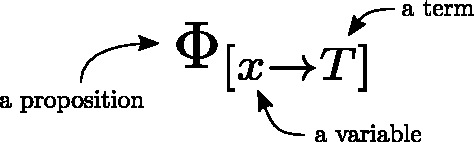
\includegraphics[scale=0.8]{img/subst.pdf}\end{center}
Some examples:
\indented{
\eg{$x\in A\cup B$}{x}{y}{$y\in A\cup B$}\lsp
\eg{$x\in A\cup B$}{A}{x}{$x\in x\cup B$}\lsp
\eg{$z^2=z+y$}{z}{a+y}{$(a+y)^2=(a+y)+y$}\lsp
\eg{$a+b\in B$}{c}{3}{$a+b\in B$}\lsp
\eg{the product of $a$ and $b$ is even}{b}{c^2}{the product of $a$ and $c^2$ is even}
}
Observe that parentheses are added as needed to avoid ambiguity.

\paragraph{A Clarification}
(If you find this remark to be more confusing than clarifying, then please feel free to skip this paragraph for now.)
What \emph{is} the string of symbols ``$\SUBST{\pA}{x}{y}$''? What part of speech are we looking at here?
It's almost a proposition, in that you get a proposition once you carry out the substitution that involves replacing $x$ by $y$.
But the string of symbols ``$\SUBST{\pA}{x}{y}$'' is not itself a proposition.
It's more like a set of \emph{instructions} telling you how to obtain a certain proposition.
The string of symbols ``$\SUBST{\pA}{x}{y}$''
has no part of speech because it is in fact not a part of the mathematical language at all!
Instead, it is part of the language we are currently using to communicate. That is, it is a part of the English
language in which this document is written, and it will help us in our mission to \emph{specify} the language of mathematics.
You can think of ``$\SUBST{\pA}{x}{y}$'' as simply a shorthand for the instruction 
\indented{
\emph{Take the proposition ``$\pA$'' and replace each copy of the variable ``$x$'' with the symbol ``$y$'', and then write the resulting proposition.}
}

\paragraph{More on substitution is coming later.}
There is a little more to substitution than simple mechanical replacement of symbols.
I've left out some important details in this section.
Take a look at these examples:
\indented{
\eg{$\ALL{x}{x=2}$}{x}{y}{$\ALL{x}{x=2}$}\lsp
\eg{$(x\in A)\AND\EXIST{x}{x=2}$}{x}{y}{$(y\in A)\AND\EXIST{x}{x=2}$}\lsp
\eg{$a\in \COLL{a}{a^2=z}$}{a}{3}{$3\in \COLL{a}{a^2=z}$}
}
In these examples, substitution does not work as you might expect. 
You might guess from the examples that the barbell symbol ``$\bbel$'' has a hand in the strange substitution rules.
We are not ready to dig into these details just yet. Later
in section \ref{sec:subst_again}, there will be more on ``$\bbel$'' and its effect on substitution.
For now, rest assured that the substitutions in the upcoming exercise are all straightforward ones--
there will be no funny business with barbells.


\ex{
For each of the following, write the proposition that results from the substitution.
\begin{enumerate}
\item $\SUBST{\text{``\ $\frac{a+b}{x+y}>x^2$\ ''}}{x}{A+B}$
\item $\SUBST{\text{``\ $B\neq B$\ ''}}{B}{y}$
\item $\SUBST{\text{``\ $z\in\{\alpha,\beta,\gamma\}$\ ''}}{\beta}{\gamma^{-1}}$
\item $\SUBST{\text{``\ $f\subseteq A\times B$\ ''}}{f}{g\circ f}$
\item $\SUBST{\text{``\ $x\in y\ARR x\in z$\ ''}}{x}{3}$
\item $\SUBST{\text{``\ $a=2\OR a=3$\ ''}}{b}{5}$
\item $\SUBST{\pB}{b}{5}$, where $\pB$ is the proposition ``$b\times b\subseteq J$''
\item $\SUBST{\text{``\ $n^2$ is even\ ''}}{n}{1}$
\item $\SUBST{\text{``\ $n^2$ is even\ ''}}{n}{n+1}$
\item $\SUBST{\SUBST{\text{``\ $n^2\REL k$\ ''}}{n}{j+k}}{k}{3}$
\end{enumerate}
}

\ex{
Is $\SUBST{\SUBST{\pA}{x}{y}}{y}{x}$ always the same as $\pA$? Explain.
}




\subsection{Universal and Existential Quantifiers}

\def\lsp{\\[0.3em]}
\newcommand{\EGENTRY}[2]{#1\hspace{1em} & #2\lsp}

\paragraph{Universal Quantifiers}
\hypertarget{hl:UQ}{Given} a proposition $\pA$ and a variable $x$, we can form
the \emph{universally quantified} proposition
$$
\ALL{x}{\pA},
$$
which is expressed in English as ``for all $x$, $\pA$.''
Typically the proposition $\pA$ would somehow involve the variable $x$.
Here are some examples, along with their expressions in English:
\indented{
\begin{tabular}{ll}
\EGENTRY{
$\ALL{x}{x=x}$
}{
For all $x$, $x=x$.
}
\EGENTRY{
$\ALL{n}{n>x}$
}{
For all $n$, $n>x$.
}
\EGENTRY{
$\ALL{y}{\text{($y$ is green)}\AND\text{($y$ is a flower)}}$
}{
For all $y$, $y$ is green and $y$ is a flower.
}
\EGENTRY{
$\ALL{y}{\text{($y$ is a flower)}\ARR\text{($y$ is green)}}$
}{
For all $y$, if $y$ is a flower then $y$ is green.
}
\end{tabular}
}

\def\BLANK{\underline{\hspace{8pt}}}

In each proposition, the variable behind the ``$\bbel$'' is said to be \emph{quantified}.
The quantified variable is special in that it's really just a placeholder.
The proposition ``$\ALL{x}{x=x}$'' is no different from
``$\ALL{y}{y=y}$''.
We might as well write them both as as
``$\ALL{\BLANK}{\BLANK=\BLANK}$'',
with the understanding that the blanks all refer to the same thing.
It is always possible to express universally quantified propositions in English
\emph{without mentioning the quantified variable},
as in the following renderings of the four examples from above:
\indented{
Everything equals itself.\lsp
Everything is greater than $x$.\lsp
Everything is a green flower.\lsp
All flowers are green.
}
Now let's get into how ``$\forall$'' is used in proofs.

\paragraph{Universal Instantiation}
\hypertarget{hl:UI}{If} you know that $\ALL{x}{\pA}$ holds, then
you can deduce $\pA$.
In fact, you can deduce \emph{any} proposition
that results from the substitution $\SUBST{\pA}{x}{\boxsubscript{20}{term}}$,
where \emph{any} term can be put in the box.
For example,
if you know that $\ALL{x}{\text{$x$ is even}}$, then
you can deduce ``$x$ is even'', and you can also deduce
things like ``$3$ is even'' and ``$A+B$ is even''.

\paragraph{Universal Generalization}
\hypertarget{hl:UG}{To} \emph{prove} a universally quantified proposition $\ALL{x}{\pA}$,
prove $\pA$ in a context in which you have made \emph{no assumptions} about the quantified variable $x$.
In such a context, the variable $x$ is said to be \emph{arbitrary}.
For example, let's say you are trying to prove that $\ALL{x}{\text{$x$ is green}}$.
Your argument could be formatted something like this:
\indented{
Consider any $x$.
\indented{
[insert argument establishing that $x$ is green]
}
Since $x$ was arbitrary, we conclude that $\ALL{x}{\text{$x$ is green}}$.
In other words, everything is green.
}
Upon reaching that first line, ``Consider any $x$,'' there are no assumptions about $x$.
If there were previous assumptions about $x$ in the larger context of the proof, then
they no longer apply after that line because \emph{this is a new and arbitrary $x$} that we are now talking about.

\paragraph{Existential Quantifiers}
\hypertarget{hl:EQ}{Given} a proposition $\pA$ and a variable $x$, we can form
the \emph{existentially quantified} proposition
$$
\EXIST{x}{\pA},
$$
which is expressed in English as ``there exists an $x$ such that $\pA$.''
Here are some examples, along with their expressions in English:
\indented{
\begin{tabular}{ll}
\EGENTRY{
$\EXIST{x}{x=x}$
}{
There exists an $x$ such that $x=x$.
}
\EGENTRY{
$\EXIST{n}{n>x}$
}{
There exists an $n$ such that $n>x$.
}
\EGENTRY{
$\EXIST{y}{\text{($y$ is green)}\AND\text{($y$ is a flower)}}$
}{
There exists a $y$ such that $y$ is green and $y$ is a flower.
}
\EGENTRY{
$\EXIST{y}{\text{($y$ is a flower)}\ARR\text{($y$ is green)}}$
}{
There exists a $y$ such that if $y$ is a flower then $y$ is green.
}
\end{tabular}
}

Again, the variable behind the ``$\bbel$'' is said to be \emph{quantified},
and it serves as a mere placeholder in the proposition.
It is always possible to express existentially quantified propositions in English
\emph{without mentioning the quantified variable},
as in the following renderings of the four examples from above:
\indented{
Something equals itself.\lsp
Something is greater than $x$.\lsp
There exists a green flower.\lsp
There exists something with the property that if it is a flower, then it is green.
}
Now let's get into how ``$\exists$'' is used in proofs.

\paragraph{Existential Generalization}
\hypertarget{hl:EG}{To} prove that $\EXIST{x}{\pA}$, all you need to do is
prove $\pA$ or some variant of $\pA$ such as $\SUBST{\pA}{x}{\boxsubscript{20}{term}}$,
in which a particular term sits in place of $x$. In other
words, to prove that ``there exists an $x$ such that $\pA$,''
you must \emph{find} an $x$, such that $\pA$.

Suppose someone tells you that there's no such thing as a spotted hamster.
Disagreeing, you reach into your pocket and pull out a spotted hamster,
proving that in fact there \emph{exists} a spotted hamster.
That is existential generalization.

\paragraph{Existential Instantiation}
\hypertarget{hl:EI}{If} you know that $\EXIST{x}{\pA}$ holds,
then \emph{as long the variable $x$ was not previously used in your proof},
you may bring $\pA$ into your argument.
That is, it is valid to assume $\pA$ for the rest of your argument.
If the variable $x$ was already in use in your proof, then to avoid a conflict of variables you would have to
introduce a brand new variable, say ``$y$'', and then from $\EXIST{x}{\pA}$ you may bring
$\SUBST{\pA}{x}{y}$ into your argument.

This is one of the trickiest manipulations with quantifiers, and it will take some getting used to.
As an example, suppose you knew for a fact that $\EXIST{x}{\text{$x$ is green}}$,
and you want to use this fact to argue that $\pC$.
Then your argument could be formatted like this:
\indented{
Since we know that $\EXIST{x}{\text{$x$ is green}}$, it is possible
to \emph{get} an $x$ such that $x$ is green.
  \indented{
  [insert argument using the fact that $x$ is green to deduce $\pC$]
  }
}
You can think of it like this:
If you and the person you are trying to convince both agree that there exists a green thing,
then you can work with a \emph{hypothetical} green thing, without needing to specify it,
in order to draw some conclusions to which you would both agree.
The key word in the example formatting above is ``get.''
It's almost like you're instructing the reader of your proof to
``go get a green thing, and then come back so we can continue the argument using that green thing.''
Except, no one ever really has to get an actual green thing; working with a hypothetical one called ``$x$''
is sufficient to run the argument.

\paragraph{Quantifying over Fewer Things}
Sometimes you don't want to say that \emph{everything} is green, 
but you want to say that everything of a certain \emph{type} is green.
Maybe you want to say that all \emph{flowers} are green, rather than all \emph{things}.
The way to express this with $\forall$ is to use $\ARR$, like this:
$$ \ALL{x}{(\text{$x$ is a flower})\ARR(\text{$x$ is green})}. $$
It is still the case that the quantified variable $x$ can be replaced by \emph{anything}.
The quantified proposition still says
``for all \emph{things}, if that thing is a flower then it is green.''
However, the implication ``$(\text{$x$ is a flower})\ARR(\text{$x$ is green})$''
only says something interesting when $x$ is a flower;
otherwise it is \emph{vacuously} true.
For this reason,
``$ \ALL{x}{(\text{$x$ is a flower})\ARR(\text{$x$ is green})}. $'' is typically expressed in English as
\begin{center}``All flowers are green.''\end{center}
What if we wanted to say that 
\emph{some} flower is green? Would
``$
\EXIST{x}{(\text{$x$ is a flower})\ARR(\text{$x$ is green})}
$''
work?
Not at all! In fact, the latter proposition would be true as long as there is at least one non-flower.
Instead of $\ARR$, to say ``some flower is green'' we should use $\AND$, like this:
$$
\EXIST{x}{(\text{$x$ is a flower})\AND(\text{$x$ is green})}.
$$
In summary: If you want to restrict the class of things you are quantifying over, then
use $\ARR$ with $\forall$, and use $\AND$ with $\exists$.

\ex{\label{ex:boundvars}
Express each of the following propositions in English without ever mentioning the quantified variable.
Insisting that the quantified variable not be mentioned can make the phrasing awkward for some of the more complicated propositions, but so be it.
\begin{enumerate}
\item $\ALL{x}{\text{ $x$ is good }}$
\item $\EXIST{x}{\text{ $x$ is good }}$
\item $\ALL{x}{(\text{ $x$ is a human })\AND(\text{ $x$ is mortal })}$
\item $\ALL{x}{(\text{ $x$ is a human })\OR (\text{ $x$ is mortal })}$
\item $\ALL{x}{(\text{ $x$ is a human })\ARR(\text{ $x$ is mortal })}$
\item $\ALL{x}{(\text{ $x$ is mortal  })\ARR(\text{ $x$ is a human })}$
\item $\EXIST{x}{(\text{ $x$ is a human })\AND(\text{ $x$ is mortal })}$
\item $\EXIST{x}{(\text{ $x$ is a human })\OR (\text{ $x$ is mortal })}$
\item $\EXIST{x}{(\text{ $x$ is a human })\ARR(\text{ $x$ is mortal })}$
\item $\ALL{x}{\neg(\text{ $x$ is good })}$
\item $\neg\ALL{x}{\text{ $x$ is good }}$
\item $\EXIST{x}{\neg(\text{ $x$ is good })}$
\item $\neg\EXIST{x}{\text{ $x$ is good }}$
\item $\ALL{x}{\text{ $x$ loves $y$ }}$
\item $\EXIST{x}{\text{ $x$ loves $y$ }}$
\item $\ALL{y}{\text{ $x$ loves $y$ }}$
\item $\EXIST{y}{\text{ $x$ loves $y$ }}$
\item $\ALL{x}{\EXIST{y}{\text{ $x$ loves $y$ }}}$\\
Hint: Work from the inside towards the outside. So start by eliminating the mention of $y$, for example by writing it as $\ALL{x}{\text{$x$ loves something}}$.
Then try to express that in English without mentioning $x$.
\item $\EXIST{y}{\ALL{x}{\text{ $x$ loves $y$ }}}$
\item $\ALL{x}{(\text{$x$ is a flower})\ARR\EXIST{y}{(\text{$y$ is a petal of $x$})\AND(\text{$y$ is green})}}$
\item $\EXIST{x}{(\text{$x$ is a flower})\AND\ALL{y}{(\text{$y$ is a petal of $x$})\ARR(\text{$y$ is green})}}$
\end{enumerate}
}



\ex{
Write each of the following using quantifier notation (i.e. using $\forall$ and $\exists$).
\begin{enumerate}
\item All birds can fly.
\item Some bird can fly.
\item Everything that can fly is a bird.
\item All birds that can fly have wings.
\end{enumerate}
}



% run through the rules and some useful derived rules of logic
% the focus is not formal derivation, but rather to make the rules intuitive and to examine how they influence *writing*
% where truth tables can help make rules intuitive, bring them in. otherwise truth tables are not a main focus
% a section on and,or,not,implies,iff,forall,exists.
% for each:
  %what it makes prop mean. 
  %what you get from having it and how to write that.
  %how to prove it and how to write that.
  %example using english props
  %useful ways it interacts with previous ones.
  %exercises

% don't forget about excluded middle and other such rules... where do those go?


% a comment (maybe put this earlier) on how repetitiveness is okay for now, and better to fix it later. perhaps sian comments on how fix

\subsection{Derived Logical Rules for Quantifiers}
\label{sec:derived2}

\setlength{\columnseprule}{1pt}

\makeatletter
\newcommand{\DrawLine}{%
  \begin{tikzpicture}
  \path[use as bounding box] (0,0) -- (\linewidth,0);
  \draw[color=black,dashed,dash phase=2pt]
        (0-\kvtcb@leftlower-\kvtcb@boxsep,0)--
        (\linewidth+\kvtcb@rightlower+\kvtcb@boxsep,0);
  \end{tikzpicture}%
  }
\makeatother

% title, statement, statement alt, pf, pf alt
\newcommand{\DRULEPFalt}[5]{
  \begin{tcolorbox}[title=Derived Rule \putRuleNumber: #1,colbacktitle=white,coltitle=black,colback=white] 
      {#2}\\
  \DrawLine\\[0.5em]
    \textbf{Proof:} {#4}\\
  \DrawLine\\[0.5em]
      \textit{A particular instance of the derived rule:}\\
      {#3}\\
  \DrawLine\\[0.5em]
    \textbf{Proof:} {#5}
  \end{tcolorbox}
}

% old side-by-side method that i'm tossing
%\newcommand{\DRULEPFalt}[5]{
%  \begin{tcolorbox}[title=Derived Rule \putRuleNumber: #1,colbacktitle=white,coltitle=black,colback=white] 
%    \begin{multicols}{2}
%      {#2}
%    \vfill
%    \columnbreak
%      {#3}
%    \end{multicols} 
%  \tcblower 
%    \begin{multicols}{2}
%      \textbf{Proof:} {#4}
%    \vfill
%    \columnbreak
%      \textbf{Proof:} {#5}
%    \end{multicols} 
%  \end{tcolorbox}
%}


\newcommand{\RELONEA}[1]{#1\text{ is green}}
\newcommand{\RELTWOA}[2]{#1\text{ loves }#2}

We now continue to derive logical rules, as we were doing in section
\ref{sec:derived1}.
This time, the rules involve quantifiers.
Like in section 
\ref{sec:derived1},
we will still not work with actual mathematical propositions,
instead favoring more general \emph{placeholders} for propositions, like $\pA$, $\pB$, etc.
However, I think that the arguments in this section can become difficult to follow if we adhere strictly to this level of generality.
For this reason, we will sometimes also include a version of the arguments that contains generic-sounding
English propositions, like ``$\RELONEA{x}$,'' or ``$\RELTWOA{x}{y}$.''
These will often appear alongside the strictly general derivations; you are welcome to follow
whichever version you find to be more convenient.


\DRULEPFalt{Global Existence Implies Local Existence}{
$\EXIST{y}{\ALL{x}{\pA}}\ARR\ALL{x}{\EXIST{y}{\pA}}$
}{
$\EXIST{y}{\ALL{x}{\text{$y$ loves $x$}}}\ARR\ALL{x}{\EXIST{y}{\text{$y$ loves $x$}}}$\\
(In other words: If there is something that loves everything, then everything is loved by something.)
}{
Assume that
$\EXIST{y}{\ALL{x}{\pA}}$.
Then we can get a $y$ such that
$\ALL{x}{\pA}$.
Now consider any $x$.
Since $\ALL{x}{\pA}$, we know that in particular $\pA$ holds.
Since we have found $y$ such that $\pA$ holds,
we can conclude that $\EXIST{y}{\pA}$.
Since $x$ was arbitrary, we can conclude that
$\ALL{x}{\EXIST{y}{\pA}}$.
}{
Assume that $\EXIST{y}{\ALL{x}{\text{$y$ loves $x$}}}$.
That is, assume that there is something that loves everything.
Then we can get something that loves everything; call it $y$.
Now consider any $x$.
Since $y$ loves everything, we know in particular that that $y$ loves $x$.
Thus \emph{something} loves $x$. That is,
$\EXIST{y}{\text{$y$ loves $x$}}$.
Since $x$ was arbitrary, we can conclude that
\emph{everything} is loved by something.
That is,
$\ALL{x}{\EXIST{y}{\text{$y$ loves $x$}}}$.
}

\newcommand{\highlight}[1]{{\color{red}#1}}

In the argument above you can see all four of the fundamental rules involving quantifiers: universal instantiation (UI),
universal generalization (UG), existential instantiation (EI), and existential generalization (EG).
Here is a repeat of the last argument with those rules pointed out:
\indented{
Assume that $\EXIST{y}{\ALL{x}{\text{$y$ loves $x$}}}$.
That is, assume that there is something that loves everything.
Then we can get \highlight{(EI)} something that loves everything; call it $y$.
Now consider any $x$.
Since $y$ loves everything, we know in particular \highlight{(UI)} that that $y$ loves $x$.
Thus \emph{something} \highlight{(EG)} loves $x$. That is,
$\EXIST{y}{\text{$y$ loves $x$}}$.
Since $x$ was arbitrary, we can conclude \highlight{(UG)} that
\emph{everything} is loved by something.
That is,
$\ALL{x}{\EXIST{y}{\text{$y$ loves $x$}}}$.
}

As you study the arguments in this section, try to identify exactly where UI, UG, EI, and EG are being used.

Regarding the derived rule above, the converse cannot be proven!
It may be useful to look at what goes wrong if we attempt to prove it anyway:
\indented{
A failed attempt to prove that
$\ALL{x}{\EXIST{y}{\text{$y$ loves $x$}}}\ARR\EXIST{y}{\ALL{x}{\text{$y$ loves $x$}}}$:\\[0.3em]
Assume that $\ALL{x}{\EXIST{y}{\text{$y$ loves $x$}}}$.
Consider any $x$.
Since $\ALL{x}{\EXIST{y}{\text{$y$ loves $x$}}}$,
we know in particular (UI) that $\EXIST{y}{\text{$y$ loves $x$}}$.
Thus we can get (EI) a $y$ such that $y$ loves $x$.
{\color{red} Since $x$ was arbitrary,
we have established (UG)}
that $\ALL{x}{\text{$y$ loves $x$}}$.
That is, $y$ loves everything.
Since we have found a $y$ that loves everything, we can conclude (EG)
that 
$\EXIST{y}{\ALL{x}{\text{$y$ loves $x$}}}$.
}
The error in the proof is colored in red. Do you see what is wrong with it?
It should feel wrong to you-- before reading on you might want to take a moment and consider what it is that feels wrong in the argument.

In order to generalize from a statement about $x$ to a statement about \emph{all} $x$, there must be no prior assumption attached to $x$.
There must be nothing special about $x$. It must be that $x$ is truly \emph{arbitrary}.
Here, however, the variable $x$ stopped being arbitrary as soon as we introduced a specific $y$ into the proof, a $y$ that loves $x$.
The $y$ loves \emph{that} particular $x$, and it does not make sense to generalize from this fact and deduce that $y$ loves \emph{everything}.

%That was kind of subtle, right?
%Of the rules UI, UG, EI, and EG, there are two subtle ones. UG is subtle, as we just saw, in that it requires that a variable really be arbitrary before
%a generalization is made. The other subtle one is EI
The error in applying UG was really subtle, and it would have been quite difficult to catch in strictly general proof written in terms of ``$\pA$''.
This is why we will often include specific English propositions like ``$y$ loves $x$'' as an aide.
It's actually fairly technical to work with quantifiers in a completely general pure logic setting.


Besides the proof, there is also a lesson that we can draw from the derived rule itself:
when multiple quantifiers are involved, be careful with the order in which you write them!

We do not need to worry about order when the same type of quantifier is repeated, as we will see in the next two rules.





\DRULEPF{Irrelevance of order of $\forall$}{
$\ALL{x}{\ALL{y}{\pA}}\ARR\ALL{y}{\ALL{x}{\pA}}$
%}{
%$\ALL{x}{\ALL{y}{\RELTWOA{x}{y}}}\ARR\ALL{y}{\ALL{x}{\RELTWOA{x}{y}}}$
}{
Assume that $\ALL{x}{\ALL{y}{\pA}}$.
Consider any $y$.
Consider any $x$.
From $\ALL{x}{\ALL{y}{\pA}}$ we can conclude ${\ALL{y}{\pA}}$, and from that we can conclude $\pA$.
Since we deduced $\pA$ while $x$ is arbitrary, we can conclude that ${\ALL{x}{\pA}}$.
Since we deduced 
${\ALL{x}{\pA}}$
while $y$ is arbitrary, we can conclude that $\ALL{y}{\ALL{x}{\pA}}$.
}

It should be intuitive that $\ALL{x}{\ALL{y}{\text{$x$ loves $y$}}}$ is the same as
$\ALL{y}{\ALL{x}{\text{$x$ loves $y$}}}$, since they both mean ``everything loves everything.''
The same goes for ``something loves something,'' derived next:

\DRULEPF{Irrelevance of order of $\exists$}{
$\EXIST{x}{\EXIST{y}{\pA}}\ARR\EXIST{y}{\EXIST{x}{\pA}}$
%}{
%$\ALL{x}{\ALL{y}{\RELTWOA{x}{y}}}\ARR\ALL{y}{\ALL{x}{\RELTWOA{x}{y}}}$
}{
Assume that $\EXIST{x}{\EXIST{y}{\pA}}$.
We can get an $x$ such that 
$\EXIST{y}{\pA}$.
Now we can get a $y$ such that
$\pA$.
Since we have found an $x$ such that $\pA$, we can conclude 
$\EXIST{x}{\pA}$.
Since we have found a $y$ such that
$\EXIST{x}{\pA}$,
we can conclude 
$\EXIST{y}{\EXIST{x}{\pA}}$.
}

We will often use the following shorthand for repeated quantifiers:
$\ALL{x,y}{\pA}$ will stand for $\ALL{x}{\ALL{y}{\pA}}$,
and similarly
$\EXIST{x,y}{\pA}$ will stand for $\EXIST{x}{\EXIST{y}{\pA}}$.

Now that we've looked at how quantifiers interact with each other, the rest of this section
explores the interaction between quantifiers and our old friends $\AND$, $\OR$, $\neg$, and $\ARR$.

\DRULEPFalt{Quantifiers and Implication 1}{
If $\ALL{x}{\pA\ARR\pB}$, then $\ALL{x}{\pA}\ARR\ALL{x}{\pB}$.
}{
If $\ALL{x}{\text{$x$ is a bird}\ARR\text{$x$ can fly}}$, then
$\ALL{x}{\text{$x$ is a bird}}\ARR\ALL{x}{\text{$x$ can fly}}$.\\
\textit{In other words:}\\
If all birds can fly, then it must be that if everything is a bird then everything can fly.
}{
Assume that $\ALL{x}{\pA\ARR\pB}$.
Assume that $\ALL{x}{\pA}$ (for the sake of proving that $\ALL{x}{\pB}$).
Consider any $x$.
Since $\ALL{x}{\pA}$, we have in particular that $\pA$. % UI
Since $\ALL{x}{\pA\ARR\pB}$, we have in particular that $\pA\ARR\pB$. % UI
From $\pA$ and $\pA\ARR\pB$, we conclude that $\pB$.
Since $x$ remains arbitrary, we may generalize to conclude that $\ALL{x}{\pB}$. % UG
}{
Assume that all birds can fly.
Assume that everything is a bird-- our goal is now to establish that everything can fly.
Consider any $x$.
Since everything is a bird, we have in particular that $x$ is a bird.
Since all birds can fly, we have in particular that if $x$ is a bird then $x$ can fly.
Therefore $x$ can fly.
Since $x$ remains arbitrary, we may generalize to conclude that \emph{everything} can fly. 
}

The above argument contains two uses of UI and one use of UG.

\ex{
The converse of the rule above cannot be established.
In fact, in the real world in which we live, (1) it is true that
if everything is a bird then everything can fly, but (2) it is false that all birds can fly.
Explain how the assertions (1) and (2) hold for our reality.
}


\DRULEPFalt{Quantifiers and Implication 2}{
If $\ALL{x}{\pA\ARR\pB}$, then $\EXIST{x}{\pA}\ARR\EXIST{x}{\pB}$.
}{
If $\ALL{x}{\text{$x$ is a bird}\ARR\text{$x$ can fly}}$, then
$\EXIST{x}{\text{$x$ is a bird}}\ARR\EXIST{x}{\text{$x$ can fly}}$.\\
\textit{In other words:}\\
If all birds can fly, then it must be that if a bird exists then something can fly.
}{
Assume that $\ALL{x}{\pA\ARR\pB}$.
Assume that $\EXIST{x}{\pA}$ (for the sake of proving that $\EXIST{x}{\pB}$).
Then we can get an $x$ such that $\pA$. %EI
Since $\ALL{x}{\pA\ARR\pB}$, we have in particular that $\pA\ARR\pB$. % UI
From $\pA$ and $\pA\ARR\pB$, we conclude that $\pB$.
Since we have found an $x$ such that $\pB$, we conclude that $\EXIST{x}{\pB}$. % EG
}{
Assume that all birds can fly.
Assume that there exists a bird-- our goal is now to establish that there exists something that can fly.
Since a bird exists, let's get one and call it $x$.
Since all birds can fly, we have in particular that if $x$ is a bird then $x$ can fly.
Therefore $x$ can fly.
Since we have found something $x$ that can fly, we conclude that \emph{something} can fly. 
}

The above argument contains a use of EI, a use of UI, and a use of EG.

\ex{
The converse of the rule above cannot be established.
In fact, in the real world in which we live, (1) it is true that
if there exists a bird then something can fly, but (2) it is false that all birds can fly.
Explain how the assertions (1) and (2) hold for our reality.
}

\ex{
There are at least two errors in the following foolish attempt to establish a converse to the rule above.
Find at least one of them, and explain why it is an error. If you are stuck, consider reading a bit more of this section
and then returning to this exercise.
\indented{
Assume that if $\EXIST{x}{\text{$x$ is a bird}}$, then $\EXIST{x}{\text{$x$ can fly}}$.
We shall now attempt to prove that $\ALL{x}{\text{$x$ is a bird}\ARR\text{$x$ can fly}}$.
Consider any $x$ and assume that $x$ is a bird.
Then \emph{something} is a bird, so  $\EXIST{x}{\text{$x$ is a bird}}$.
It follows that $\EXIST{x}{\text{$x$ can fly}}$.
%Since $\EXIST{x}{\text{$x$ is a bird}}$, we can get a bird; call this bird $x$.
Since $\EXIST{x}{\text{$x$ can fly}}$, we can get something that can fly; call this something $x$.
Since $x$ is a bird and it can fly, we have proven that $\text{$x$ is a bird}\ARR\text{$x$ can fly}$.
Since $x$ is arbitrary, we can generalize to conclude that $\ALL{x}{\text{$x$ is a bird}\ARR\text{$x$ can fly}}$. 
}
}

\DRULEPFalt{Quantifiers and Conjunction 1}{
If $\EXIST{x}{\pA\AND\pB}$, then $\EXIST{x}{\pA}\AND\EXIST{x}{\pB}$.
}{
If $\EXIST{x}{\text{$x$ is a flower}\AND\text{$x$ is green}}$, then $\EXIST{x}{\text{$x$ is a flower}}$ and $\EXIST{x}{\text{$x$ is green}}$.\\
\textit{In other words:}\\
If there exists a green flower, then something is a flower and something is green.
}{
Assume that $\EXIST{x}{\pA\AND\pB}$.
Then we can get an $x$ such that $\pA\AND\pB$. % EI
Since we have found an $x$ such that $\pA$, we can conclude that $\EXIST{x}{\pA}$. % EG
Since we have found an $x$ such that $\pB$, we can conclude that $\EXIST{x}{\pB}$. % EG
Thus $\EXIST{x}{\pA}$ and $\EXIST{x}{\pB}$.
}{
Assume that there exists a green flower. Then we can get a green flower, call it $x$.
Since $x$ is a flower, we have found a flower and we can conclude that there exists a flower.
Since $x$ is green, we have found a green thing and we can conclude that there exists a green thing.
Thus something is a flower and something is green.
}

The above argument contains a use of EI and two uses of EG.

It should be intuitive that the converse doesn't work.
If a flower exists and a green thing exists, then we cannot necessarily conclude that a green flower exists.
It could be that our world is full of non-green flowers and green non-flowers, but contains no green flowers.
We can learn something by trying to prove the converse anyway, and looking for the error:
\indented{
Assume that $\EXIST{x}{\text{$x$ is a flower}}$ and $\EXIST{x}{\text{$x$ is green}}$.
We shall now attempt to prove that $\EXIST{x}{\text{$x$ is a flower}\AND\text{$x$ is green}}$.
Since $\EXIST{x}{\text{$x$ is a flower}}$, we can get (EI) a flower; let's call it $x$.
Since also $\EXIST{x}{\text{$x$ is green}}$, we can get (EI) a green thing; let's call that $x$ as well.
Since $x$ is a green flower, we have found a green flower and we can conclude (EG) that $\EXIST{x}{\text{$x$ is a flower}\AND\text{$x$ is green}}$.
}

Before reading on you might want to take a moment and consider what exact part of the argument feels wrong, and what is wrong with it.

...


\newpage


The error is in the second use of EI. Recall that when you use EI to go from $\EXIST{x}{\pA}$ to $\pA$,
the variable $x$ cannot already be in use. If it is in use, then you have to substitute in a new variable such as $y$, and then you can bring
$\SUBST{\pA}{x}{y}$ into the argument.
The critical error in the argument given here is in ``let's call that $x$ as well,'' which is where we decided to name the green thing $x$.
We should have used a different name, like $y$,
since we only knew that we could get \emph{some} green thing and we should not allow that to conflict with the name $x$ that we gave to our hypothetical flower.
If we had called the flower $x$ and the green thing $y$, then there would be no way for the argument to proceed, and all's right with the world.


\DRULEPFalt{Quantifiers and Conjunction 2}{
$\ALL{x}{\pA\AND\pB}$ if and only if $\ALL{x}{\pA}\AND\ALL{x}{\pB}$.
}{
$\ALL{x}{\text{$x$ is large}\AND\text{$x$ is green}}$ if and only if $\ALL{x}{\text{$x$ is large}}$ and $\ALL{x}{\text{$x$ is green}}$.\\
\textit{In other words:}\\
Everything is large and green if and only if everything is large and everything is green.
}{
$\Rightarrow$: Assume that $\ALL{x}{\pA\AND\pB}$.
Consider any $x$. Since $\ALL{x}{\pA\AND\pB}$, we have in particular that $\pA\AND\pB$ % UI
Since $x$ is arbitrary and we have $\pA$, we conclude that $\ALL{x}{\pA}$. % UG
Since $x$ is arbitrary and we have $\pB$, we conclude that $\ALL{x}{\pB}$. % UG
Thus $\ALL{x}{\pA}\AND\ALL{x}{\pB}$.

$\Leftarrow$: Assume that $\ALL{x}{\pA}\AND\ALL{x}{\pB}$.
Consider any $x$.
Since $\ALL{x}{\pA}$, we have in particular that $\pA$. % UI
Since $\ALL{x}{\pB}$, we have in particular that $\pB$. % UI
Since we now have $\pA\AND\pB$ and since $x$ is arbitrary, we may generalize to conclude that $\ALL{x}{\pA\AND\pB}$. % UG
}{
$\Rightarrow$: Assume that everything is large and green.
Consider any $x$. Since everything is large and green, we know in particular that $x$ is large and green.
Since $x$ is arbitrary and we showed that it is large, we may generalize to conclude that everything is large.
Similarly, since $x$ is arbitrary and we showed that it is green, we may generalize to conclude that everything is green.
Thus everything is large and everything is green.
\lsp

$\Leftarrow$: \putExerciseHeading:
Prove that if everything is large and everything is green, then it follows that everything is large and green.
Hint: your argument should involve two uses of UI and one use of UG.
}


\def\lsp{\\[-0.1em]}
\def\ADJA{dry}
\def\ADJB{hot}

% LXXI ii do
\DRULEPFalt{Quantifiers and Disjunction 1}{
If $\ALL{x}{\pA}\OR\ALL{x}{\pB}$,
then $\ALL{x}{\pA\OR\pB}$.
}{
If $\ALL{x}{\text{$x$ is \ADJA{}}}\OR\ALL{x}{\text{$x$ is \ADJB{}}}$,
then $\ALL{x}{\text{$x$ is \ADJA{}}\OR\text{$x$ is \ADJB{}}}$.\\
\textit{In other words:}\\
If either everything is \ADJA{} or everything is \ADJB{}, then everything is either \ADJA{} or \ADJB{}.
}{
Assume that $\ALL{x}{\pA}\OR\ALL{x}{\pB}$.\lsp

Case 1: Assume that $\ALL{x}{\pA}$. Consider any $x$.
Since $\ALL{x}{\pA}$, it follows in particular that $\pA$. 
Thus we have $\pA\OR\pB$, and since $x$ is arbitrary we may generalize and conclude that $\ALL{x}{\pA\OR\pB}$.\lsp

Case 2: Assume that $\ALL{x}{\pB}$. Consider any $x$.
Since $\ALL{x}{\pB}$, it follows in particular that $\pB$. 
Thus we have $\pA\OR\pB$, and since $x$ is arbitrary we may generalize and conclude that $\ALL{x}{\pA\OR\pB}$.\lsp

Since we ended up with $\ALL{x}{\pA\OR\pB}$ in both cases, we may conclude that $\ALL{x}{\pA\OR\pB}$.
}{
Assume that either everything is \ADJA{} or everything is \ADJB{}.\lsp

Case 1: Suppose that everything is \ADJA{}. Consider any $x$.
Since everything is \ADJA{}, $x$, in particular, is \ADJA{}.
Thus $x$ is \ADJA{} or it is \ADJB{}. Since $x$ is arbitrary, we may generalize and conclude that \emph{everything} is either \ADJA{} or \ADJB{}.\lsp

Case 1: Suppose that everything is \ADJB{}. Consider any $x$.
Since everything is \ADJB{}, $x$, in particular, is \ADJB{}.
Thus $x$ is \ADJA{} or it is \ADJB{}. Since $x$ is arbitrary, we may generalize and conclude that \emph{everything} is either \ADJA{} or \ADJB{}.\lsp

Since both cases lead us to conclude that everything is either \ADJA{} or \ADJB{}, we can go ahead and conclude that everything is either \ADJA{} or \ADJB{}.
}


The above argument contains a use of UI and two uses of UG.

% LXXI ii (the above) converse give wrong proof and make ex to find error.
It should be intuitive that the converse doesn't work.
If everything is either \ADJA{} or \ADJB{}, then it does not necessarily follow
that either everything is \ADJA{} or everything is \ADJB{}.
There could still be some \ADJA{} things that aren't \ADJB{} as well as some \ADJB{} things that aren't \ADJA{}.

\ex{
Here is an attempt at arguing for the converse. What is the exact mistake?
\indented{
Assume that everything is either \ADJA{} or \ADJB{}.
We will attempt to prove that either everything is \ADJA{}, or everything is \ADJB{}. 
Consider any $x$. Since everything is \ADJA{} or it is \ADJB{}, we know that $x$, in particular, is either \ADJA{} or \ADJB{}.

Case 1: Suppose that $x$ is \ADJA{}. Then, since $x$ is arbitrary, we may generalize and conclude that everything is \ADJA{}.
It follows that either everything is \ADJA{} or everything is \ADJB{}.

Case 2: Suppose that $x$ is \ADJB{}. Then, since $x$ is arbitrary, we may generalize and conclude that everything is \ADJB{}.
It follows that either everything is \ADJA{} or everything is \ADJB{}.

Since we concluded in both cases that everything is \ADJA{} or everything is \ADJB{}, we can go ahead and conclude that everything is \ADJA{} or everything is \ADJB{}.
}
}


% LXXI i do, but leave one direction of englishy portion as an ex
\DRULEPFalt{Quantifiers and Disjunction 2}{
$\EXIST{x}{\pA\OR\pB}$ if and only if $\EXIST{x}{\pA}\OR\EXIST{x}{\pB}$.
}{
$\EXIST{x}{\text{$x$ is \ADJA{}}\OR\text{$x$ is \ADJB{}}}$ if and only if $\EXIST{x}{\text{$x$ is \ADJA{}}}\OR\EXIST{x}{\text{$x$ is \ADJB{}}}$.\\
\textit{In other words:}\\
``Something is either \ADJA{} or \ADJB{}'' is equivalent to ``Either something is \ADJA{}, or something is \ADJB{}.''
}{
$\Rightarrow$: Assume that $\EXIST{x}{\pA\OR\pB}$.
We may then get an $x$ such that $\pA\OR\pB$.\lsp

Case 1: Suppose that $\pA$. Since we have found an $x$ such that $\pA$, we may conclude that $\EXIST{x}{\pA}$.
It follows that $\EXIST{x}{\pA}\OR\EXIST{x}{\pB}$.\lsp

Case 2: Suppose that $\pB$. Since we have found an $x$ such that $\pB$, we may conclude that $\EXIST{x}{\pB}$.
It follows that $\EXIST{x}{\pA}\OR\EXIST{x}{\pB}$.\lsp

Since both cases led us to conclude that $\EXIST{x}{\pA}\OR\EXIST{x}{\pB}$, we may go ahead and conclude that $\EXIST{x}{\pA}\OR\EXIST{x}{\pB}$.\lsp

$\Leftarrow$: \putExerciseHeading.
}{
$\Rightarrow$: Assume that something is either \ADJA{} or \ADJB{}.
We may then get an $x$ which is either \ADJA{} or \ADJB{}.\lsp

Case 1: Suppose that $x$ is \ADJA{}. Since we have found an $x$ that is \ADJA{}, we may conclude that \emph{something} is \ADJA{}.
It follows that either something is \ADJA{} or something is \ADJB{}.\lsp

Case 2: Suppose that $x$ is \ADJB{}. Since we have found an $x$ that is \ADJB{}, we may conclude that \emph{something} is \ADJB{}.
It follows that either something is \ADJA{} or something is \ADJB{}.\lsp

Since both cases led us to conclude that either something is \ADJA{} or something is \ADJB{}, we may go ahead and conclude that
either something is \ADJA{} or something is \ADJB{}.

$\Leftarrow$: \putExerciseHeading.
}










% LXXXIX iii and iv: do one, leave the entire other one as an exercise.
\def\ADJA{good}
\DRULEPFalt{
Quantifiers and Negation 1
}{
$\neg\ALL{x}{\pA}\DARR\EXIST{x}{\neg\pA}$
}{
$\neg\ALL{x}{\text{$x$ is \ADJA{}}}\DARR\EXIST{x}{\text{$x$ is not \ADJA{}}}$\\
\textit{In other words:}
``Not everything is \ADJA{}'' is equivalent to ``Something is not \ADJA{}.''
}{
$\Leftarrow$:
Assume that $\EXIST{x}{\neg\pA}$.
Suppose, for the sake of obtaining a contradiction, that $\ALL{x}{\pA}$.
Since $\EXIST{x}{\neg\pA}$,
we can get an $x$ such that $\neg\pA$.
Since $\ALL{x}{\pA}$, we have in particular that $\pA$.
Having arrived at the contradiction $\pA\AND\neg\pA$, we find that we must reject $\ALL{x}{\pA}$.
That is, $\neg\ALL{x}{\pA}$.
\lsp

$\Rightarrow$:
For this direction we will prove the contrapositive $\neg\EXIST{x}{\neg\pA}\ARR\ALL{x}{\pA}$
(see Derived Rule \ref{drule:contraposition}).
Assume that $\neg\EXIST{x}{\neg\pA}$.
Consider any $x$.
\lsp

Suppose, for the sake of contradiction, that $\neg\pA$.
Then we found an $x$ such that $\neg\pA$, so we may conclude that
$\EXIST{x}{\neg\pA}$. We've reached the contradiction $\EXIST{x}{\neg\pA}\AND\neg\EXIST{x}{\neg\pA}$.
Therefore we must reject $\neg\pA$ and we see that in fact $\pA$.\lsp

Since we've established $\pA$ for an arbitrary $x$, we can generalize to conclude that $\ALL{x}{\pA}$.
}{
$\Leftarrow$:
Assume that something is not \ADJA{}.
Suppose, for the sake of obtaining a contradiction, that everything is \ADJA{}.
Since something is not \ADJA{}, we can get a non-\ADJA{} thing and call it $x$.
Since everything is \ADJA{}, we have in particular that $x$ is \ADJA{}.
This is a contradiction-- $x$ cannot be both \ADJA{} and not \ADJA{}.
Thus we reject the assumption that everything is \ADJA{}.
That is, not everything is \ADJA{}.\lsp

$\Rightarrow$:
We would like to prove that if not everything is \ADJA{}, then something is not \ADJA{}.
By contraposition, it suffices to prove that if it's \emph{not} the case that something is not \ADJA{}, then everything must be \ADJA{}.
Assume that it's not the case that something is not \ADJA{}.
Consider any $x$.
\lsp

Suppose, for the sake of contradiction, that $x$ is not \ADJA{}.
Then we found an $x$ that is not \ADJA{}, so we may conclude that
something is not \ADJA{}.
But we now have a contradiction-- it both is and isn't the case that something is not \ADJA{}.
Therefore we must reject $x$ is not \ADJA{} and we see that in fact $x$ must be \ADJA{}.
\lsp

Since we've established that $x$ is \ADJA{} for arbitrary $x$, we can generalize to conclude that \emph{everything} is \ADJA{}.
}


\DRULEPFalt{
Quantifiers and Negation 2
}{
$\neg\EXIST{x}{\pA}\DARR\ALL{x}{\neg\pA}$
}{
$\neg\EXIST{x}{\text{$x$ is \ADJA{}}}\DARR\ALL{x}{\text{$x$ is not \ADJA{}}}$\\
\textit{In other words:}
``Nothing is \ADJA{}'' is equivalent to ``Everything is not \ADJA{}.''
}{
Apply ``Quantifiers and Negation 1'' to the proposition $\neg\pA$ (putting $\neg\pA$ in place of $\pA$) to obtain
$\neg\ALL{x}{\neg\pA}\DARR\EXIST{x}{\pA}$.
Then invert this equivalence (see Derived Rule \ref{drule:neg_equiv}) to obtain the desired equivalence.
}{
\putExerciseHeading: Write this proof without relying on ``Quantifiers and Negation 1.''
Your argument could look pretty similar to the argument that
``Not everything is \ADJA{}'' is equivalent to ``Something is not \ADJA{},''
which is given in ``Quantifiers and Negation 1.''
}



\def\hsp{\hspace{1em}}

\hypertarget{hl:NOTUSE}{The} two rules above, along with Derived Rules
\ref{drule:demorgan1},
\ref{drule:demorgan2},
and \ref{drule:neg_impl}
form a complete toolkit
for ``pushing'' $\neg$ into complicated propositions.
For example, here are the stages of
negating $\ALL{x}{\pA\ARR(\pB\OR\EXIST{y}{\pC})}$
and pushing the negation inward:
$$\begin{array}{ll}
\neg\ALL{x}{\pA\ARR(\pB\OR\EXIST{y}{\pC})} \hsp &\DARR\\
\EXIST{x}{\neg(\pA\ARR(\pB\OR\EXIST{y}{\pC}))} \hsp &\DARR\\
\EXIST{x}{\pA\AND\neg(\pB\OR\EXIST{y}{\pC})} \hsp &\DARR\\
\EXIST{x}{\pA\AND\neg\pB\AND\neg\EXIST{y}{\pC}} \hsp &\DARR\\
\EXIST{x}{\pA\AND\neg\pB\AND\ALL{y}{\neg\pC}}. &
\end{array}$$
Here's the exact same procedure with $\pA$ replaced by ``$x$ is a flower'', $\pB$ replaced by ``$x$ is purple'', and $\pC$ replaced by ``$y$ is a green petal of $x$'':
\begin{center}
\begin{tabular}{ll}
``It is not the case that all flowers are either purple or have a green petal'' \hsp &iff\\
``There is something for which it is not the case that if it is a flower then &\\
             \hspace{2em} it is either purple or it has a green petal '' \hsp &iff\\
``There is some flower for which it is not the case that it is either purple&\\
             \hspace{2em} or it has a green petal'' \hsp &iff\\
``There is some non-purple flower which does not have a green petal'' \hsp &iff\\
``There is some non-purple flower all of whose petals are non-green'' &
\end{tabular}
\end{center}
Hopefully the overall negation feels intuitive, even if the individual steps in pushing the negation are a little awkward.


% exercise: now that we know how to push neg into quantifiers, do it to a bunch of these (some are in english and some are more symbolic, one of them is the analysis one)
% remind about derived rule that converts "unless" to "if" and to use that.

% all and
% all or
% exist and
% exist or
% exist implies
% all implies
% an interesting all-exist,
% an interesting exist-all
% the analysis one 
% same as all above above but English
% (do some shuffling, but keep the ones with more quantifiers below ones with less)


\ex{\label{ex:neg_quant1}
Negate each of the following propositions, and push the negation into the innermost component propositions.
Recall from Derived Rule \ref{drule:unless} that $\neg\pA\OR\pB$ can be rewritten as $\pA\ARR\pB$.
When you encounter things like $\neg\pA\OR\pB$, you can rewrite them in terms of ``$\ARR$''
in order to reduce the overall number of ``$\neg$'' symbols.
\begin{enumerate}

\item %5
$\ALL{x}{\pA\ARR\pB}$ 


\item %4
$\EXIST{x}{\pA\OR\pB}$ 

\item %1
$\ALL{x}{\pA\AND\pB}$ 

\item %2
$\ALL{x}{\pA\OR\pB}$ 


\item %6
$\EXIST{x}{\pA\ARR\pB}$ 

\item %3
$\EXIST{x}{\pA\AND\pB}$ 


\item %7
$\ALL{x}{\pA\ARR\EXIST{y}{\pB\AND(\pC\OR\pD)}}$

\item %8
$\EXIST{x}{\pA\AND\pB\AND\ALL{y}{\pC\ARR\pD}}$

\item %9
$\ALL{x}{\pA\ARR\EXIST{y}{\pB\AND\ALL{z}{\pC\ARR\pD}}}$

\end{enumerate}
}

\ex{\label{ex:neg_quant2}
Again negate each of the following propositions, pushing the negation into the innermost component propositions.
Whenever you see the English ``or'' being used, remember that it actually stands for the mathematical ``$\OR$''
and not whatever sort of ``or'' would suit a conversational context.
\begin{enumerate}

\item %1e
Everything is warm and fuzzy.

\item %2e
Everything is either good or it is bad.

\item %4e
There is something which is either a dog or a wolf.

\item %7e
Every person has a friend who is either very skinny or very fat. 

\item %3e
Some bird can fly.

\item %9e
Every company has at least one committee whose members are all loyal to the company.

\item %5e
Every bird can fly.

\item %6e
There exists something with the property that if it is a bird, then it can fly.

\item %8e
Some flower is green and has all of its petals being pointy.

\end{enumerate}
}

\ex{
Each proposition in Exercise \ref{ex:neg_quant2} is actually modeled on exactly one
proposition from Exercise \ref{ex:neg_quant1}-- ``modeled on'' in the sense that
$\pA$, $\pB$, etc. have been replaced by some specific propositions in English.
Can you match them up?
For each proposition in Exercise \ref{ex:neg_quant2}, figure out which proposition in Exercise \ref{ex:neg_quant1} it was modeled on.
}








\subsection{Substitution Revisited}
\label{sec:subst_again}

Now that we've thoroughly explored quantifiers, we can better understand the anomalous substitution examples
from the end of section \ref{sec:subst}. Here is one of those anomalous substitutions:
\indented{
\eg{$\ALL{x}{\text{$x$ is good}}$}{x}{y}{$\ALL{x}{\text{$x$ is good}}$}
}
Why didn't the $x$ symbol physically get replaced by $y$ when the substitution was carried out?
Well, the proposition $\ALL{x}{\text{$x$ is good}}$ simply says that everything is good.
If we do physically replace every ``$x$'' mark with a ``$y$'' then it still says that everything is good.
Since the meaning doesn't change anyway, substitution does not need to affect the $x$. If we \emph{did} allow the substitution to affect the $x$,
this would cause problems in examples like the following:
$$
\ALL{x}{\text{$x$ loves $y$}}.
$$
This proposition asserts that everything loves $y$. If we now replace each physical $x$ mark by a $y$, then we end up with 
$$
\ALL{y}{\text{$y$ loves $y$}},
$$
which asserts something totally different: everything loves \emph{itself}!
Formally, we design our substitution rules so that the barbell ``$\bbel$'' protects the variable preceding it from being replaced in a substitution.
A variable that is guarded by a barbell is said to be a \emph{bound} variable of the proposition that it is in.
Otherwise it is said to be a \emph{free} variable.
Free variables can get affected by substitution; for example making the substitution
$[y\rightarrow z]$
in
``$\ALL{x}{\text{$x$ loves $y$}}$''
yields 
``$\ALL{x}{\text{$x$ loves $z$}}$.''
This works as intended: if you take ``everything loves $y$'' and replace $y$ with a $z$ you should get ``everything loves $z$.''

However, there is yet another subtlety involving substitutions which can lead to unintended consequences.
Consider the substitution
$[y\rightarrow x]$
in
``$\ALL{x}{\text{$x$ loves $y$}}$''.
This time $y$ is free variable, and there is no ``$\bbel$'' to protect it from being replaced,
so the substitution
yields
``$\ALL{x}{\text{$x$ loves $x$}}$''.
Again we find that a simple variable replacement has drastically changed the meaning of what's being asserted!
This is not supposed to happen.
In mathematical logic, certain substitutions are considered to be ``unacceptable.''
All substitution troubles can be avoided if, 
whenever you make a substitution,
you \emph{never replace a bound variable} and you \emph{never use a bound variable in a replacement}.

%To stop it from happening, we deem the 
%substitution to be... unacceptable. 
%We could start filling pages with formal rules regarding which substitutions are acceptable, but it's sufficient to leave a general warning for now:
%\textit{When you make a substitution, unless you really know what you're doing,
%do not replace a bound variable or even use a bound variable in a replacement.}

\paragraph{Free and Bound Variables}
When you read a mathematical proposition, it's a very good thing to be aware of which variables are free and which variables are bound. 
Free variables are \emph{really there} in the proposition in which they appear,
whereas bound variables are more like \emph{dummy} variables.
For example, in the proposition ``$\EXIST{x}{\text{$x$ loves $y$}}$'' we have a free variable $y$ and a bound variable $x$.
The proposition is really saying something about $y$; it says that there is something that loves $y$, something that specifically loves $y$.
But it says nothing about $x$. The proposition doesn't really involve $x$, even though an ``$x$'' symbol is physically present.
As you saw in Exercise \ref{ex:boundvars}, a proposition with bound variables can be expressed in English without mentioning any of the bound variables--
that's because it's just not saying anything about those variables.

The terminology of ``free'' and ``bound'' variables also gives us an interesting way to think about how UI, UG, EI, and EG
work in written proofs.
When you use EI to go from
``$\EXIST{x}{\text{$x$ loves $y$}}$''
to
``$x$ loves $y$''
in a proof, you are in some sense \emph{freeing} the bound variable $x$.
You go from ``\emph{something} loves $y$'' to ``$x$ loves $y$''.
You go from some unspecified unnamed thing that loves $y$, to a specific thing called $x$ that loves $y$.
In written proofs, EI and UI free up bound variables, while EG and UG \emph{bind} free variables.

\paragraph{Implicit Universal}
\hypertarget{hl:implicitU}{Suppose} you prove a theorem with some free variables in it.
Say you've proven ``If $x$ and $y$ are odd, then $x+y$ is even.''
This has $x$ and $y$ as free variables, so it looks like it's making a statement specifically about $x$ and $y$.
But they are still \emph{variables}, and they are \emph{arbitrary}; that's because they appear in a standalone theorem statement
with no external assumptions.
Thus UG applies and you can generalize to deduce
\begin{equation}\label{eq:implicitU1}
\ALL{x,y}{\text{if $x$ and $y$ are odd, then $x+y$ is even}}.
\end{equation}
Now there are no free variables, and indeed the theorem can be expressed in an English sentence that has no variables:
``The sum of two odd things is even.''
Mathematicians are actually more likely to state the theorem as 
\begin{equation}\label{eq:implicitU2}
\text{if $x$ and $y$ are odd, then $x+y$ is even}.
\end{equation}
with free $x$ and $y$, rather than explicitly including the ``$\forall x,y$'' as in (\ref{eq:implicitU1}).
It's just easier to write this way, and everyone understands that since $x$ and $y$ are arbitrary, there's sort of an
implicit ``$\forall x,y$'' that could be included.

Recall that UI allows you to deduce $\SUBST{\pA}{x}{\boxsubscript{20}{term}}$ from $\ALL{x}{\pA}$, for any term that you'd like to have replace $x$.
For example you can deduce
\begin{equation}\label{eq:implicitU3}
\text{if $5$ and $z+1$ are odd, then $5+(z+1)$ is even}
\end{equation}
from (\ref{eq:implicitU1}),
which itself was deduced from (\ref{eq:implicitU2}).
The bottom line is that if you've proven $\pA$ as a theorem, then you can substitute any terms you like for the free variables in $\pA$, and you would also
have proven the resulting proposition.
\DRULE{Variable Substitution}{
Given $\pA$, if $x$ is \emph{arbitrary} then you can deduce $\SUBST{\pA}{x}{\boxsubscript{20}{term}}$,
where any term can sit in the box labeled ``term.''
(For example, all free variables would be arbitrary if $\pA$ is already proven as a standalone theorem, so free variables
in a theorem can freely be replaced by terms.)
}



% Variables live to serve. Their purpose in life is to either be bound, or to be free and to eventually be replaced in a substition.


 

% here include a version of how pronouns work
% how there's an implicit "for all" in a lot of theorem statements, but it's really not needed to say it due to how pronouns work

% and also go into those details on bound vs free variables, and how barbells block substitution
% (you can look at the crazy nested quantifiers special case in jacoby notes)

\subsection{Logic Summary}
\label{sec:logic_summary}

% here put a table with each of the logical operators, including quantifiers, along with columns such as:
%  symbol, english statement, how to use, how to prove, things to watch out for, useful related derived rules (perhaps just the number refs, which are clickable links)
% make table entries be clickable links that reference parts of the document.

Here is a reference table for each of the logical constructions that we've looked at.
Many of the table entries will be clickable references if your pdf reader supports hyperlinks.

\def\cellwidth{8em}
\def\vpad{\\[-0.3em]}
\renewcommand{\arraystretch}{2.8} % Default value: 1

\begin{tabular}{c|c|c|c|c}
\textbf{name} &
\textbf{symbolic} &
\textbf{English} &
\textbf{to prove} &
\textbf{to use} 
\\\hline
\hyperlink{hl:AND}{conjunction} &
$\pA\AND\pB$ &
$\pA$ and $\pB$ &
\parbox{\cellwidth}{\hyperlink{hl:ANDPV}{prove $\pA$ and\\ prove $\pB$}\vpad} &
\parbox{\cellwidth}{\hyperlink{hl:ANDUSE}{can deduce $\pA$ and can deduce $\pB$}\vpad} 
\\\hline
\hyperlink{hl:OR}{disjunction} &
$\pA\OR\pB$ &
$\pA$ or $\pB$ &
\parbox{\cellwidth}{\hyperlink{hl:ORPV}{prove $\pA$ or\\ prove $\pB$}\vpad} &
\parbox{\cellwidth}{\hyperlink{hl:ORUSE}{proof by cases}\vpad} 
\\\hline
\hyperlink{hl:NOT}{negation} &
$\neg\pA$ &
\parbox{6em}{it is not the\\ case that $\pA$\vpad} &
\parbox{\cellwidth}{\hyperlink{hl:NOTPV}{proof by\\ contradiction}\vpad} &
\parbox{\cellwidth}{\hyperlink{hl:NOTUSE}{push the $\neg$ in before using}\vpad} 
\\\hline
\hyperlink{hl:ARR}{implication} &
$\pA\ARR\pB$ &
 $\pB$ if $\pA$ &
\parbox{\cellwidth}{\hyperlink{hl:ARRPV}{assume $\pA$,\\ then prove $\pB$}\vpad} &
\parbox{\cellwidth}{\hyperlink{hl:ARRUSE}{given $\pA$,\\ can deduce $\pB$}\vpad} 
\\\hline
\hyperlink{hl:DARR}{equivalence} &
$\pA\DARR\pB$ &
\parbox{5em}{$\pA$ if and\\ only if $\pB$\vpad} &
\parbox{\cellwidth}{\hyperlink{hl:DARRPV}{prove both\\implications}\vpad} &
\parbox{\cellwidth}{\hyperlink{hl:DARRUSE}{know whether $\pA$\\ based on $\pB$}\vpad} 
\\\hline
\hyperlink{hl:UQ}{universal} &
$\ALL{x}{\pA}$ &
for all $x$, $\pA$ &
\parbox{\cellwidth}{\hyperlink{hl:UG}{universal\\generalization}\vpad} &
\parbox{\cellwidth}{\hyperlink{hl:UI}{universal\\instantiation}\vpad} 
\\\hline
\hyperlink{hl:EQ}{existential} &
$\EXIST{x}{\pA}$ &
for some $x$, $\pA$ &
\parbox{\cellwidth}{\hyperlink{hl:EG}{existential\\generalization}\vpad} &
\parbox{\cellwidth}{\hyperlink{hl:EI}{existential\\instantiation}\vpad} 
\end{tabular}
\renewcommand{\arraystretch}{1} % Set back to default

\section{Set Theory} % and still writing though...
\label{sec:sets}

Recall that the game of mathematics consists of starting points, which are the axioms,
and ways of generating new results from the starting points, which are the rules of deduction.
In the previous section, we established all the rules of deduction.
In this section, we will introduce axioms and generate some results from them.




\subsection{Membership, Inclusion, and Equality}

\AXIOMN{Reflexiveness for Equality\label{ax:refl_eq}}{$x=x$.}

\AXIOMN{Equality Used\label{ax:eq_used}}{
If $x=y$, then $\SUBST{\pA}{a}{x}\DARR\SUBST{\pA}{a}{y}$.
}

\THMN{Symmetry and Transitivity for Equality\label{thm:sym_trans_eq}}{
\begin{enumerate}[(1)]
\item\label{thm:sym_trans_eq1}
If $x=y$, then $y=x$.
\item\label{thm:sym_trans_eq2}
If $x=y$ and $y=z$, then $x=z$.
\end{enumerate}
}
\proofnewline
\textit{Proof of \ref{thm:sym_trans_eq1}:}
Assume that $x=y$.
Applying Axiom \ref{ax:eq_used}
to the proposition ``$a=x$'' shows us that $x=x$ if and only if $y=x$.
Since $x=x$ by Axiom \ref{ax:refl_eq}, it follows that $y=x$.
\done
\proofsep
\textit{Proof of \ref{thm:sym_trans_eq2}:}
Assume that $x=y$ and $y=z$.
Apply Axiom \ref{ax:eq_used}
to the proposition ``$a=z$'' and the equality $x=y$.
This gives us that $x=z$ if and only if $y=z$.
Since $y=z$ by hypothesis, it follows that $x=z$.
\done

\paragraph{Fewer Axioms is Better}
Why should ``$x=x$'' be an axiom while symmetry and transitivity are theorems?
Are symmetry and transitivity not just as fundamental to the meaning of equality as reflexiveness?
Well, we could have set up Theorem \ref{thm:sym_trans_eq} as an axiom instead, and then we wouldn't
have needed to bother with a proof.
But we prefer to keep the axioms to a minimum.
If we \emph{can} derive a result from previous results, then we choose to do so.

Otherwise, why not just make everything an axiom and save some effort?
To do so would be terribly boring.
The interesting part of mathematics is in seeing what \emph{follows} from one's assumptions.
It is somehow satisfying to know that equality \emph{must} be symmetric and transitive
if it is to satisfy $x=x$ and allow for substitution.
It would not have been possible to set up the rules of the game so as to exclude symmetry and transitivity for equality.

Another motivation for having fewer axioms is \emph{consistency}.
If it is possible to prove a contradiction within our mathematical framework, then
the entire framework is said to be \emph{inconsistent}.
This would be absolutely disastrous; recall Rule \ref{rule:contradictions}.
We really \emph{hope} that it is impossible to prove a contradiction from our axioms,
but the more axioms we introduce the worse our confidence becomes that it is impossible to prove a contradiction.

One can also think about it in strategic terms.
When you make an argument to convince someone of your view,
it only works if they agree
with the premises of your argument.
This is more likely when there are fewer premises.
If mathematics is one giant argument that is being made,
then the axioms are the premises of that argument.

\paragraph{Using Equality on Propositions and Terms}
Axiom \ref{ax:eq_used} tells us that if we know $x=y$, then we can replace $x$ by $y$ in any proposition to obtain an
equivalent proposition.
Axiom \ref{ax:eq_used} also allows for variable replacements in \emph{terms} and not just propositions.
If $x=y$ then here is how Axiom \ref{ax:eq_used} allows us to argue that $x^2=y^2$:
Assume that $x=y$ and apply Axiom \ref{ax:eq_used} to the proposition ``$a^2=y^2$''.
We get that $x^2=y^2$ if and only if $y^2=y^2$. Since $y^2=y^2$ due to Axiom \ref{ax:refl_eq},
it follows that $x^2=y^2$.

In summary:
If $x=y$, then replacing $x$ by $y$ in a \emph{proposition} gives a \emph{logically equivalent} proposition,
and replacing $x$ by $y$ in a \emph{term} gives an \emph{equal} term. We package these ideas into one handy theorem,
whose proof is just a general application of the idea above:

\def\tA{\smiley{}}

\THMNP{Equality Used\label{thm:eq_used}}{In
this theorem, we use ``$\tA$''  as a placeholder for a \emph{term},
just like we use ``$\pA$'' as a placeholder for a \emph{proposition}.
So we can apply parts
\ref{itm:eq_used:2}
and
\ref{itm:eq_used:4}
below
to a specific situation by
replacing each copy of ``$\tA$'' by a chosen term,
just as we can obtain specific instances of parts
\ref{itm:eq_used:1}
and
\ref{itm:eq_used:3}
by replacing each ``$\pA$'' by a chosen proposition.
\\[0.5em]
If $x=y$, then:
\begin{enumerate}[(1)]
\item \label{itm:eq_used:1} $\SUBST{\pA}{a}{x}\DARR\SUBST{\pA}{a}{y}$
\item \label{itm:eq_used:2} $\tA_{[a\rightarrow x]}=\tA_{[a\rightarrow y]}$
\item \label{itm:eq_used:3} $\pA\DARR\SUBST{\pA}{x}{y}$
\item \label{itm:eq_used:4} $\tA=\tA_{[x\rightarrow y]}$
\end{enumerate}
}{
Assume that $x=y$. Part \ref{itm:eq_used:1} is just Axiom \ref{ax:eq_used}.

To prove part 
\ref{itm:eq_used:2},
apply Axiom \ref{ax:eq_used}
to the proposition ``$\tA_{[a\rightarrow x]}=\tA$'' and to the fact that $x=y$.
We get that
$$ \SUBST{(\tA_{[a\rightarrow x]}=\tA)}{a}{x}\ \DARR\ \SUBST{(\tA_{[a\rightarrow x]}=\tA)}{a}{y}. $$
Carrying out a substitution instruction involves applying the substitution to every part of an expression,
so here we must apply the substitutions to the individual expressions on both sides of the ``$=$''.
Thus we have
$$ (\SUBST{\tA_{[a\rightarrow x]}}{a}{x}=\SUBST{\tA}{a}{x})\ \DARR\ (\SUBST{\tA_{[a\rightarrow x]}}{a}{y}=\SUBST{\tA}{a}{y}). $$
After carrying out the substitution $\SUBST{\tA}{a}{x}$, there will be no free ``$a$'' left to be further replaced in a substitution, so
$\SUBST{\tA}{a}{x}$, $\SUBST{\SUBST{\tA}{a}{x}}{a}{x}$, and $\SUBST{\SUBST{\tA}{a}{x}}{a}{y}$ all result in the same string
of symbols.
We therefore have
$$ (\SUBST{\tA}{a}{x}=\SUBST{\tA}{a}{x})\ \DARR\ (\SUBST{\tA}{a}{x}=\SUBST{\tA}{a}{y}). $$
Since the left hand side of this holds by Axiom \ref{ax:refl_eq}, we conclude that $\SUBST{\tA}{a}{x}=\SUBST{\tA}{a}{y}$.

To prove \ref{itm:eq_used:3},
simply apply \ref{itm:eq_used:1},
with ``$x$'' playing the role of ``$a$''.
We get $\SUBST{\pA}{x}{x}\DARR\SUBST{\pA}{x}{y}$.
Noting that $\SUBST{\pA}{x}{x}$ is $\pA$, we have $\pA\DARR\SUBST{\pA}{x}{y}$.

To prove \ref{itm:eq_used:4},
simply apply \ref{itm:eq_used:2},
with ``$x$'' playing the role of ``$a$''.
We get $\SUBST{\tA}{x}{x}=\SUBST{\tA}{x}{y}$.
Noting that $\SUBST{\tA}{x}{x}$ is $\tA$, we have $\tA=\SUBST{\tA}{x}{y}$.
}

\paragraph{How to Gain Equality?}
The axioms so far give us a mechanism for using and manipulating equalities.
But where can we get some equalities to play with in the first place (other than ones like $x=x$)?
How can we \emph{prove} an interesting equality?
This will be addressed shortly in Axiom \ref{ax:eq_gain}; we first need to get membership into the picture.

\paragraph{Notation}
The proposition ``$a\in b$'' is read as ``$a$ is in $b$'' or ``$a$ is an element of $b$.''
The term ``$\COLL{x}{\pA}$'' is read as ``the set of $x$ such that $\pA$.''
The appearance of ``$\bbel$'' suggests that ``$x$'' is a \emph{bound} variable in the term ``$\COLL{x}{\pA}$'',
and indeed it is! Terms of this form can be expressed in English without any mention of the bound variable.
For example $\COLL{x}{\text{$x$ is green}}$ could be referred to as ``the set of green things,'' with no mention of $x$.
Also, the bound variable can be replaced without any change in meaning: the term ``$\COLL{y}{\text{$y$ is green}}$''
refers just as much to ``the set of green things.''
The following axiom establishes how $\in$ and $\COLL{x}{\pA}$ work.

\AXIOMN{\label{ax:in}Membership}{
$a\in\COLL{x}{\pA}\DARR\SUBST{\pA}{x}{a}$.\\
\textit{Warning: this axiom is broken.}
}

The notation $\COLL{x}{\pA}$ serves to ``collect'' together all the $x$'s for which $\pA$ holds.
A set $\COLL{x}{\pA}$ is like an exclusive club, and $\pA$ is the condition for membership in that club.
Various propositions could go in the position of $\pA$ to create collections like the following:
\indented{
$\COLL{x}{\text{$x$ is a person} \AND\EXIST{y}{\text{$y$ is a friend of $x$}}}$
\hspace*{1em}\hfill
The set of people who have a friend.\\
$\COLL{n}{3<n^2<4+x}$\hfill
The set of things whose square is strictly between $3$ and $4+x$.
}
Axiom \ref{ax:in} says that $a$ is an element of $\COLL{x}{\text{$x$ is a person} \AND\EXIST{y}{\text{$y$ is a friend of $x$}}}$
if and only if $a$ is a person and $\EXIST{y}{\text{$y$ is a friend of $a$}}$.
Axiom \ref{ax:in} says that 
$b\in\COLL{n}{3<n^2<4+x}$ if and only if $3<b^2<4+x$.

\paragraph{Broken?}
\hypertarget{hl:bug}{We} should talk about that warning.
Axiom \ref{ax:in} is the way people at one point thought they could set up set theory.
But it all came crashing down.
It turns out to be broken in the worst possible way-- Axiom \ref{ax:in} allows us to prove a contradiction.
Allowing $\pA$ to really be \emph{any} proposition does not work;
certain choices of $\pA$ seem to cause trouble.
So what do we do about this?
People have handled the bug in various ways by modifying Axiom \ref{ax:in}.
Different approaches have led to different types of set theory.
We can also choose to \emph{ignore} the bug and move on.
Then we would be doing what is called \emph{naive set theory}.
This is what we choose to do for now, while just bearing in mind that
there are some propositions $\pA$ on which Axiom \ref{ax:in} should not be used.
There will be more comments later on how to fix the bug;
most of what we do is not affected much by the fix. 
 
Moving on.

\DEFN{Inclusion}{
$a\subseteq b\DARR \ALL{z}{z\in a\ARR z\in b}$.
}

Here are some ways to read ``$a\subseteq b$'' in English:
\indented{
$a$ is a subset of $b$\\
$a$ is contained in $b$\\
$a$ is included in $b$
}
For $a$ to be a subset of $b$, every element of $a$ must be an element of $b$.
Do not confuse this with ``$a$ is in $b$,'' which is actually a way of saying ``$a\in b$''!
Explicitly using the symbols ``$\in$'' and ``$\subseteq$'', or explicitly saying ``element'' and ``subset''
can help to avoid confusion.
Here is a way to imagine the situation $x\in a$:
\begin{center}
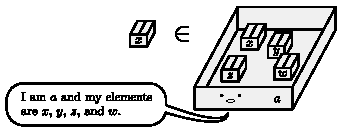
\includegraphics[scale=1.5]{img/boxes/1.pdf}
\end{center}

\begin{samepage}
And here is a way to imagine the situation $x\subseteq a$:
\begin{center}
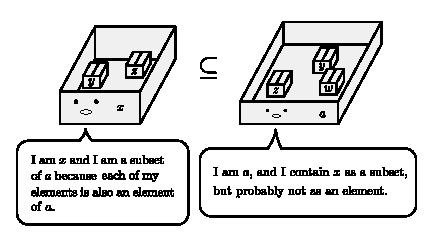
\includegraphics[scale=1.5]{img/boxes/2.pdf}
\end{center}
\end{samepage}

\paragraph{On Definitions}
Definitions are like axioms in that they serve as starting points.
But we distinguish them from axioms because all they do is provide a convenient \emph{name}
for something by introducing new symbols or terminology.
Definitions don't assert anything truly new, so they don't allow us to prove anything truly new.
More precisely, the only things a definition allows us to prove are the same things we proved before, but with old names
replaced by new names.
Definitions could be omitted from our entire framework without changing which theorems can be proven, just changing
how we are able to state those theorems.
Having too many axioms is undesirable, but there is nothing wrong with having lots of definitions.
% On defns: they are like axioms in that they serve as starting points.
% but we distinguish them from axioms because all they do conveniently *name* some new symbols in terms of old symbols
% they don't really assert anything, so they don't allow us to prove anything truly new
% the only things they allow us to prove are the same things we proved before, but with old names replaced by new names.
% definitions could be omitted completely without changing which theorems can be proven
% having too many axioms is undesirable, but there's nothing wrong with having lots of definitions

\THMN{\label{thm:refl_trans_incl}Reflexivity and Transitivity for Inclusion}{
\begin{enumerate}[(1)]
\item\label{thm:refl_trans_incl1}
$a\subseteq a$.
\item\label{thm:refl_trans_incl2}
If $a\subseteq b$ and $b\subseteq c$, then $a\subseteq c$.
\end{enumerate}
}
\proofnewline
\textit{Proof of \ref{thm:refl_trans_incl1}:}
If $z\in a$ then $z\in a$, so we have $\ALL{z}{z\in a\ARR z\in a}$.
In other words, $a\subseteq a$.
\done
\proofsep
\textit{Proof of \ref{thm:refl_trans_incl2}:}
Assume that $a\subseteq b$ and $b\subseteq c$.
To prove that $a\subseteq c$, consider any $z\in a$.
Since $a\subseteq b$, it follows that $z\in b$.
Since $b\subseteq c$, it follows further that $z\in c$.
Since we showed that $z\in c$ for an arbitrary $z\in a$, we have shown $\ALL{z}{z\in a\ARR z\in c}$.
In other words, $a\subseteq c$.
\done

In the proof of Theorem \ref{thm:refl_trans_incl} part \ref{thm:refl_trans_incl2}, you should be able to spot two uses of \hyperlink{hl:UI}{UI} and one use of \hyperlink{hl:UG}{UG}.

If $a=b$, then by Axiom \ref{ax:eq_used} we have $z\in a\DARR z\in b$, for all $z$.
So the equality $a=b$ gives both inclusions $a\subseteq b$ and $b\subseteq a$.
In other words, if $a$ and $b$ are equal then they must have exactly the same elements. 
We will take this to be the full \emph{meaning}
of equality, by taking on the converse as an axiom.

\AXIOMN{Equality Gained{\label{ax:eq_gain}}}{
If $\ALL{z}{z\in a\DARR z\in b}$, then $a=b$.
}

This makes it so that anything and everything that we can refer to in our mathematical language is nothing more than its elements.
In other words, \emph{everything is a set}:

\THMP{
$y=\COLL{z}{z\in y}$.
}{
We will show that $\ALL{w}{w\in y\DARR w\in\COLL{z}{z\in y}}$. Then we will be finished, due to Axiom \ref{ax:eq_gain}.

Consider any $w$.
Axiom \ref{ax:in} tells us that $w\in\COLL{z}{z\in y}$ holds if and only if $\SUBST{\text{``$z\in y$''}}{z}{w}$ holds.
In other words, $w\in\COLL{z}{z\in y}$ if and only if $w\in y$.
Since $w$ was arbitrary, we are done.
}

\THMNP{Equality as Double Inclusion\label{thm:eq_incl}}{
$a=b$ if and only if $a\subseteq b$ and $b\subseteq a$.
}{
$\Rightarrow$:
Assume that $a=b$.
Then by Axiom \ref{ax:eq_used} we have $z\in a\DARR z\in b$, for all $z$.
From $z\in a\ARR z\in b$ we can generalize to conclude that $\ALL{z}{z\in a\ARR z\in b}$.
In other words, $a\subseteq b$.
Similarly, from $z\in b\ARR z\in a$ we can generalize to conclude that $b\subseteq a$.

$\Leftarrow$:
Assume that $a\subseteq b$ and $b\subseteq a$.
We will show that $\ALL{z}{z\in a\DARR z\in b}$. Then we will be finished, due to Axiom \ref{ax:eq_gain}.

Consider any $z$.
From $a\subseteq b$ we have $z\in a\ARR z\in b$, and
from $b\subseteq a$ we have $z\in b\ARR z\in a$.
It follows that $z\in a\DARR z\in b$. Since $z$ is arbitrary, we are done.
}

Since equality is equivalent to two inclusions, proofs of equality are often split into two parts, with each part dedicated to proving one of the inclusions.

\begin{samepage}
Before ending this section on membership, we take a moment to point out that membership is normally not transitive;
having $y\in x$ and $x\in a$ does not allow you to conclude that $y\in a$.
\begin{center}
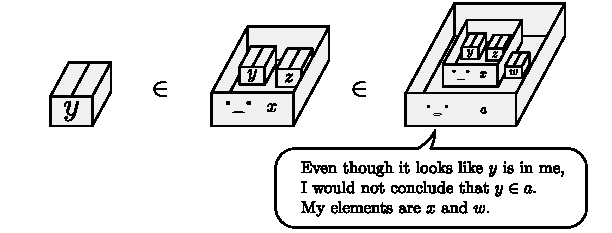
\includegraphics[scale=1.4]{img/boxes/3.pdf}
\end{center}
\end{samepage}

\ex{
For each of the following, determine if it is a term, a proposition, or nothing because it is ill-formed.
\begin{enumerate}
\item $\COLL{a}{a\in a}$
\item $\COLL{x}{x}$
\item $\COLL{y}{\ALL{z}{z\subseteq y}}$
\item $x+y\in z$
\item $a=(b\in c)$
\item $3\subseteq P$
\end{enumerate}
}

\ex{
Express each of the following sets in English without mentioning any bound variables.
\begin{enumerate}
\item $\COLL{x}{\text{$x$ is good}}$
\item $\COLL{x}{\text{$x$ loves $y$}}$
\item $\COLL{y}{\text{$x$ loves $y$}}$
\item $\COLL{z}{z\subseteq p}$
\item $\COLL{z}{\ALL{x}{x\subseteq p\ARR z\in x}}$
\end{enumerate}
}

\ex{
Prove that $a\in\COLL{k}{k=a}$.
}

\ex{
Prove that if $\COLL{k}{k=a}\subseteq m$, then $a\in m$.
}

\ex{
Let $B=\COLL{a}{a\subseteq \COLL{k}{k=b}}$. Prove that if $j\in z$ and $z\in B$, then $j=b$.
}

\ex{For this exercise, let
$$ s=\COLL{x}{\EXIST{a}{x\in a\AND a\in y}} $$
and let
$$ t=\COLL{a}{\EXIST{x}{x\in a\AND a\in y}}. $$
\begin{enumerate}
\item \label{ex:st_membership:first_s}Which variables are free in the definition of $s$ and which are bound?
\item Describe $s$ in English without mentioning any bound variables.
\item What does it mean for $z$ to be an element of $s$? (Use Axiom \ref{ax:in}.)
\item \label{ex:st_membership:last_s}What does it mean for $y$ to be an element of $s$? 
Express your answer in English without mentioning any bound variables.
\item Answer questions \ref{ex:st_membership:first_s}-\ref{ex:st_membership:last_s} for $t$ instead of $s$.
\item Assume that every element of $y$ has an element. That is, assume that $$\ALL{z}{z\in y\ARR\EXIST{w}{w\in z}}.$$
Prove that $t=y$.
\end{enumerate}
}


\subsection{Empty Set, Singletons, and Uniqueness}

\DEFN{Empty Set}{
$\emptyset = \COLL{x}{x\neq x}$
}

Here we have defined the first \hyperlink{hl:constants}{constant} of our language.

The notation $a\notin b$
is a shorthand for $\neg(a\in b)$,
and similarly $a\neq b$ is short for $\neg(a=b)$.

\THMNP{Empty Set is Empty\label{thm:emptyset_empty}}{
$x\notin\emptyset$.
}{
If $x\in \emptyset$
then $x\neq x$, but this would contradict Axiom \ref{ax:refl_eq}.
}

\THMN{Minimality of the Empty Set\label{thm:emptyset_minimal}}{
\begin{enumerate}[(1)]
\item \label{thm:emptyset_minimal1} $\emptyset\subseteq a$.
\item \label{thm:emptyset_minimal2} If $a\subseteq\emptyset$, then $a=\emptyset$.
\end{enumerate}
}
\proofnewline
\textit{Proof of \ref{thm:emptyset_minimal1}:}
Consider any $z$.
Since $z\notin\emptyset$ (Theorem \ref{thm:emptyset_empty}),
it is \hyperlink{hl:vacuous}{vacuously true} that $z\in\emptyset\ARR z\in a$.
\done
\proofsep
\textit{Proof of \ref{thm:emptyset_minimal2}:}
Assume that $a\subseteq\emptyset$.
We already have $\emptyset\subseteq a$
from part \ref{thm:emptyset_minimal1}.
Since we got both inclusions, we have proven the equality $a=\emptyset$ (Theorem \ref{thm:eq_incl}).
\done

\THMNP{Only the Empty Set is Empty\label{thm:emptyset_unique}}{
If $x\notin a$ for all $x$, then $a=\emptyset$.
}{
Assume that $\ALL{x}{x\notin a}$.
Consider any $z$.
Since $z\notin a$
by hypothesis,
it is vacuously true that $z\in a\ARR z\in\emptyset$.
Since $z$ is arbitrary, we may conclude that $a\subseteq\emptyset$.
It follows that $a=\emptyset$ (Theorem \ref{thm:emptyset_minimal}).
}

In the proof of Theorem \ref{thm:emptyset_unique}, you should be able to spot one use of \hyperlink{hl:UI}{UI} and one use of \hyperlink{hl:UG}{UG}.

Theorem \ref{thm:emptyset_unique} is an example of a \emph{uniqueness theorem}.
If you know that $g$ is green and you want to assert that $g$ is the only green thing in existence, then the way to assert that is
$$
\ALL{a}{\text{$a$ is green}\ARR a=g}.
$$
If we read ``$\ALL{x}{x\notin a}$'' as ``$a$ is empty,'' then Theorem \ref{thm:emptyset_unique} looks like this:
$$
\ALL{a}{\text{$a$ is empty}\ARR a=\emptyset}.
$$
The universal quantifier ``$\forall a$'' does not show up explicitly in the statement of Theorem \ref{thm:emptyset_unique},
but remember that \hyperlink{hl:implicitU}{it is sort of implicitly there}.

Theorem \ref{thm:emptyset_unique} tells us that ``being empty'' is the same thing as ``being equal to $\emptyset$.''
When a set is described ``nonempty,'' that is the same as saying that the set is not equal to $\emptyset$.

\THMNP{Nonemptiness\label{thm:nonempty}}{
$a\neq\emptyset\DARR\EXIST{x}{x\in a}$.
}{
$\Rightarrow$:
This implication can be established by considering the \hyperlink{hl:contraposition}{contraposition}
$$
\neg\EXIST{x}{x\in a}\ARR a=\emptyset
$$
and \hyperlink{hl:NOTUSE}{pushing the negation in} to see that it is equivalent to Theorem \ref{thm:emptyset_unique}.

$\Leftarrow$:
Assume that $\EXIST{x}{x\in a}$.
Then we can get some $x$ such that $x\in a$.
Now we cannot have $a=\emptyset$, for if we did then $x\in a$ would contradict Theorem \ref{thm:emptyset_empty}.
}

In the proof of Theorem \ref{thm:nonempty}, you should be able to spot one use of \hyperlink{hl:EI}{EI}.

\DEFN{\label{def:singleton}Singleton}{
$\{x\}=\COLL{a}{a=x}$.
}

This definition gives us an object $\{x\}$ with the property that any $a$ is an element of $\{x\}$ if and only if $a=x$.
In other words, $x$ is an element of $\{x\}$ and it is the \emph{unique} element of $\{x\}$.

\DEFN{Doubleton}{
$\{x,y\}=\COLL{a}{(a=x)\OR (a=y)}$.
}

You can probably guess how $\{x,y,z\}$ and longer ``lists of elements'' are defined:

\DEFN{More Ways to List Elements}{
\begin{enumerate}[(1)]
\item $\{x,y,z\}=\COLL{a}{(a=x)\OR (a=y)\OR (a=z)}$
\item $\{x,y,z,u\}=\COLL{a}{(a=x)\OR (a=y)\OR (a=z)\OR (a=u)}$
\item $\{x,y,z,u,v\}=\COLL{a}{(a=x)\OR (a=y)\OR (a=z)\OR (a=u)\OR (a=v)}$
\item $\{x,y,z,u,v,w\}=\COLL{a}{(a=x)\OR (a=y)\OR (a=z)\OR (a=u)\OR (a=v)\OR (a=w)}$
\end{enumerate}
}

Of course we are restricted to finite lists, because we can only write finite lists
with our finite ink and finite paper.

\THMNP{\label{thm:singleton_subset}Singleton and Inclusion}{
$x\in S$ if and only if $\{x\}\subseteq S$.
}{
$\Rightarrow$:
Assume that $x\in S$.
Consider any $z\in\{x\}$. Then $z=x$, so we have $z\in S$.
Since $z$ was arbitrary, we may conclude that $\{x\}\subseteq S$.

$\Leftarrow$:
Assume that $\{x\}\subseteq S$.
We have  $x\in \{x\}$ (since $x=x$).
Therefore we have $x\in S$. 
}


\THMPL{$\{x,y\}=\{y,x\}$}{
This essentially follows from the logical rule $\pA\OR\pB\DARR\pB\OR\pA$. Here are the details.

Consider any $z$.
We have
\begin{align*}
z\in\{x,y\} &\DARR (z=x)\OR (z=y)\\
&\DARR (z=y)\OR (z=x)\\
&\DARR z\in\{y,x\}.
\end{align*}
From $z\in\{x,y\} \DARR z\in\{y,x\}$ we generalize to conclude that $\{x,y\}=\{y,x\}$.
}{
\label{thm:dton_unord}
}

\THMPL{
$\{x\}=\{y\}$ if and only if $x=y$.
}{
$\Rightarrow$:
Assume that $\{x\}=\{y\}$.
We have $x\in\{x\}$, since $x=x$. Thus we have $x\in\{y\}$, and from this we get $x=y$.

$\Leftarrow$:
Assume that $x=y$.
%Consider any $z$.
%We have $z=x\DARR z=y$,
%so $z\in\{x\}\DARR z\in\{y\}$.
Then $\{x\}=\{y\}$, by Axiom \ref{ax:eq_used}.
}{
\label{thm:eq_ston}
}



\THMPL{
$\{x,y\}=\{u\}$ if and only if $x=y=u$.
}{
\putExerciseHeading.
}{
\label{thm:dton_eq_ston}
}



\THMPL{
If $\{x,y\}=\{u,v\}$, then either $x=u$ and $y=v$, or $x=v$ and $y=u$.
}{
\putExerciseHeading.
}{
\label{thm:eq_dton}
}


\ex{
Prove that
$\{x\}\subseteq\{x,y\}$.
}






\ex{Prove that
$\{\emptyset\}\neq \emptyset$.
}


\ex{Prove that
$\{\{\emptyset\}\}\neq \{\emptyset\}$.
}



\ex{
Prove that 
if $y=\{b\}$, then
$\COLL{z}{\EXIST{x}{(z\in x)\AND(x\in y)}}=b$.
}

\ex{Prove that if $a\subseteq\{x\}$, then either $a=\emptyset$ or $a=\{x\}$.}

\DEFN{Being a Singleton\label{def:be_singleton}}{
A set is said to be a \emph{singleton} iff it has the form $\{x\}$ for some $x$.
That is, we call $s$ a singleton iff
$\EXIST{x}{s=\{x\}}.$
}

A singleton is characterized by the fact that it contains a unique element:

\THMNP{Existence and Uniqueness in Terms of Singleton\label{thm:singleton_uniqueness}}{

A set $s$ is a singleton if and only if it has a unique element.
That is, $s$ is a singleton if and only if
$$
\EXIST{x}{x\in s\AND \ALL{y}{y\in s\ARR y=x}}.
$$}{
$\Rightarrow:$
Assume that $s$ is a singleton. Then we can get an $x$ such that $s=\{x\}$.
We have $x\in s$, by Definition \ref{def:singleton}, and it remains to prove that $\ALL{y}{y\in s\ARR y=x}$.
Consider any $y\in s=\{x\}$. Definition \ref{def:singleton} immediately gives $y=x$.

$\Leftarrow:$
Now assume that $\EXIST{x}{x\in s\AND \ALL{y}{y\in s\ARR y=x}}$.
Get an $x\in s$ such that \[\ALL{y}{y\in s\ARR y=x}.\tag{$\ast$}\label{eqn:singleton_unique}\]
We claim that $s=\{x\}$.
Since $x\in s$, we have $\{x\}\subseteq s$ by Theorem \ref{thm:singleton_subset}.
Since $y=x\DARR y\in\{x\}$, the condition (\ref{eqn:singleton_unique})
can be rewritten as ``$\ALL{y}{y\in s\ARR y\in\{x\}}$,'' which is the definition of ``$s\subseteq\{x\}$.''
Thus, having proven both inclusions, we have $s=\{x\}$.
}

\paragraph{``Getting'' Unique Things}
Often in mathematics we know that there exists a unique thing with certain properties.
How can we \emph{refer} to it?
For example, let's say we know that there exists a unique green thing.
In English, we would refer to it by saying ``\emph{the} green thing.''
Is there a mathematical version of ``the'' that can allow us to write down a \emph{term}
which refers to ``the unique such-and-such''?

If we know that $\EXIST{x}{\text{$x$ is green}}$, then we can always use \hyperlink{hl:EI}{EI}
to ``get'' a green thing $x$.
But that would just be a \emph{hypothetical} green thing that was can use for the sake of arguments.
We can use it to draw conclusions, but ``$x$'' would still not refer to any \emph{specific} green thing.
It would be ``a green thing'' and not ``the green thing.''
However, if we knew that there were a \emph{unique} green thing, i.e. if we knew
$$
\EXIST{x}{\text{$x$ is green}\AND\ALL{y}{\text{$y$ is green}\ARR y=x}},
$$
then by Theorem \ref{thm:singleton_uniqueness} we would know that 
$$
\COLL{x}{\text{$x$ is green}}
$$
is a \emph{singleton}.
This means that $\COLL{x}{\text{$x$ is green}}=\{g\}$ for some $g$, and then if we ``pluck'' $g$ out of $\{g\}$, that's
``\emph{the} green thing.''

It is therefore useful to have a formal mechanism for ``plucking'' the single occupant of a singleton out from between the curly braces.
The following definition provides this, although this may not be clear until Theorem \ref{thm:occ}.


\DEFN{Occupant\label{def:occ}}{
Let $s$ be a singleton.
The \emph{occupant} of $s$ is denoted by $\occ{s}$ and defined by
$$
\occ{s}=\COLL{z}{\ALL{x}{x\in s\ARR z\in x}}.
$$
}

The definition above contains an \emph{assumption}, that $s$ is a singleton.
When a definition contains an assumption, the definition is only meant to be used under the conditions of the assumption.
If you try to use the definition without first verifying that those conditions hold, then the definition may behave in unintended ways.
We can declare the notation to be ``undefined'' in such cases, and reject any argument that breaches into undefined territory.
We just don't talk about $\occ{s}$ unless $s$ is already known to be a singleton.

\THMNP{\label{thm:occ}Essence of Occupant}{$\occ{\{g\}}=g.$}{
$\subseteq$:
Assume that $z\in \occ{\{g\}}$.
Then for every $x\in \{g\}$, we have $z\in x$.
In particular $g\in \{g\}$, so we have $z\in g$.

$\supseteq$:
Assume that $z\in g$.
Now we must prove that $z$ is an element of every $x\in \{g\}$.
Consider any $x\in \{g\}$.
Then $x=g$, so $z\in g$ gives $z\in x$.
}

Now we have an explicit way to refer to ``the green thing,''
when we know that there is a unique green thing:
$$
\text{Let $g=\occ{\COLL{x}{\text{$x$ is green}}}$.}
$$
In practice, this is achieved by writing something like
\begin{center}
{Let $g$ denote the unique green thing.}
\end{center}

\ex{Determine what is $\occ{\COLL{x}{\ALL{y}{y\notin x}}}$, and prove your claim. If it is ``undefined,'' then say so.
Hint: Theorem \ref{thm:emptyset_unique}}.


\subsection{Intersection, Union, and Relative Complement}

\def\vsp{\vspace{0.3em}}

\DEFN{Intersection and Union}{
\vsp
\begin{enumerate}[(1)]
\item $a\cap b = \COLL{x}{(x\in a)\AND(x\in b)}$
\item $a\cup b = \COLL{x}{(x\in a)\OR (x\in b)}$
\end{enumerate}
\vsp
}

% INCLUDE THESE LINES IN THMS ONLY VERSION
\newcommand{\thmline}[2]{
\item \hspace*{1em} #1 \hfill (#2) \hspace*{2em}
}%
\newcommand{\thmlineL}[3]{
\item #3 \hspace*{1em} #1 \hfill (#2) \hspace*{2em}
}%
% END INCLUDE

\def\hsp{\hspace{0.8em}}

\THMN{Algebraic Properties of Intersection and Union\label{thm:cupcap_props}}{
\vsp
\begin{enumerate}[(1)]
\thmlineL{$a\cap b=b\cap a$}{commutativity of $\cap$}{\label{thm:cupcap_props1}}
\thmline{$a\cup b=b\cup a$}{commutativity of $\cup$}
\thmline{$(a\cap b)\cap c=a\cap (b\cap c)$}{associativity of $\cap$}
\thmline{$(a\cup b)\cup c=a\cup (b\cup c)$}{associativity of $\cup$}
\thmlineL{$a\cup (b\cap c)=(a\cup b)\cap(a\cup c)$}{$\cup$ distributes over $\cap$}{\label{thm:cupcap_props2}}
\thmline{$a\cap (b\cup c)=(a\cap b)\cup(a\cap c)$}{$\cap$ distributes over $\cup$}
\thmline{$a\cap a=a$}{idempotence of $\cap$}
\thmline{$a\cup a=a$}{idempotence of $\cup$}
\thmlineL{$a\cup \emptyset=a$}{$\emptyset$ is an identity for $\cup$}{\label{thm:cupcap_props3}}
\thmlineL{$a\cap\emptyset=\emptyset$}{$\emptyset$ is an annihilator for $\cap$}{\label{thm:cupcap_props4}}
\end{enumerate}
\vsp
}
\proofnewline
\textit{Proof of \ref{thm:cupcap_props1}:}
For any given $z$, we have
$$
z\in a\cap b
\hsp\DARR\hsp
(z\in a)\AND(z\in b)
\hsp\DARR\hsp
(z\in b)\AND(z\in a)
\hsp\DARR\hsp
z\in b\cap a.
$$
\done
\proofsep
\textit{Proof of \ref{thm:cupcap_props2}:}
For any given $z$, we have
\begin{align*}
z\in a\cup (b\cap c)
&\hsp\DARR\hsp
(z\in a) \OR (z\in b\cap c)\\
&\hsp\DARR\hsp
(z\in a) \OR ((z\in b)\AND(z\in c))\\
&\hsp\DARR\hsp
((z\in a)\OR(z\in b))\AND((z\in a)\OR(z\in c))\\
&\hsp\DARR\hsp
(z\in a\cup b)\AND(z\in a\cup c)\\
&\hsp\DARR\hsp
z\in (a\cup b)\cap(a\cup c).
\end{align*}
\done
\proofsep
\textit{Proof of \ref{thm:cupcap_props3}:}
$\supseteq$:
Consider any $z\in a$. Then we have $(z\in a)\OR(z\in\emptyset)$, so $z\in a\cup\emptyset$.

$\subseteq$:
Consider any $z\in a\cup\emptyset$.
Then we have either $z\in a$ or $z\in\emptyset$.
Since $z\notin\emptyset$, it must be that $z \in a$ (Rule \ref{DRULE:alt_elim}).
\done
\proofsep
Proving the rest of them is \putExerciseHeading.

In the proofs given above, you can see some different ways of proving an equality.
In the first two proofs, the pattern is to establish a chain of ``$\DARR$'' and then gain an equality like $A=B$
by having proven $\ALL{z}{z\in A\DARR z\in B}$.
This is relying on Axiom \ref{ax:eq_gain}.
In the third proof, the pattern is to gain $A=B$ by establishing $A\subseteq B$ and $B\subseteq A$.
This is relying on Theorem \ref{thm:eq_incl}.
The latter pattern, gaining equality via double inclusion, is far more commonly used and it will ultimately be much more useful for you.
Chains of ``$\DARR$'' really only show up in the basics of set theory-- they become very unwieldy when things get the slightest bit complicated.

\THMNP{Maximality of Intersection\label{thm:cap_max}}{
\thmStartNewline
The set $b\cap c$ is a subset of both $b$ and $c$,
and it contains anything that is a subset of both $b$ and $c$.
That is,
\begin{enumerate}[(1)]
\item $b\cap c\subseteq b$ \label{thm:cap_max1}
\item $b\cap c\subseteq c$ \label{thm:cap_max2}
\item If $a\subseteq b$ and $a\subseteq c$, then $a\subseteq b\cap c$. \label{thm:cap_max3}
\end{enumerate}
}{
To prove \ref{thm:cap_max1},
consider any $z\in b\cap c$.
Then $z\in b$ and $z\in c$. In particular, $z\in b$.

The proof of \ref{thm:cap_max2} is similar.

To prove \ref{thm:cap_max3}, assume that $a\subseteq b$ and $a\subseteq c$.
Consider any $z\in a$.
Due to our hypothesis we have $z\in b$ and $z\in c$, so
$z\in b\cap c$. Since $z$ is arbitrary, we may conclude that $a\subseteq b\cap c$.
}

\THMNP{Minimality of Union\label{thm:cup_min}}{
\thmStartNewline
The set $b\cup c$  contains both $b$ and $c$, and it is a subset of any set that contains both $b$ and $c$.
That is,
\begin{enumerate}[(1)]
\item $b\subseteq b\cup c$ \label{thm:cup_min1}
\item $c\subseteq b\cup c$ \label{thm:cup_min2}
\item If $b\subseteq a$ and $c\subseteq a$, then $b\cup c\subseteq a$. \label{thm:cup_min3}
\end{enumerate}
}{
\putExerciseHeading. A proof by cases is needed in \ref{thm:cup_min3}.
}

\THMNP{Inclusion in Terms of $\cap$ and $\cup$\label{thm:incl_capcup}}{
\thmStartNewline
The following are equivalent:
\begin{enumerate}[(1)]
\item \label{thm:incl_capcup1} $a\subseteq b$
\item \label{thm:incl_capcup2} $a\cap b=a$
\item \label{thm:incl_capcup3} $a\cup b = b$
\end{enumerate}
}{
$\ref{thm:incl_capcup1}\ARR\ref{thm:incl_capcup2}$:
Assume that $a\subseteq b$.
We already have $a\cap b\subseteq a$ by Theorem \ref{thm:cap_max},
so it remains for us to prove that $a\subseteq a\cap b$.
Consider any $z\in a$. Since $a\subseteq b$, we have $z\in b$.
Now since $z\in a$ and $z\in b$, it follows that $z\in a\cap b$.

$\ref{thm:incl_capcup2}\ARR\ref{thm:incl_capcup3}$:
Assume that $a\cap b=a$.
We already have $b\subseteq a\cup b$ by Theorem \ref{thm:cup_min},
so it remains for us to prove that $a\cup b \subseteq b$.
Consider any $z\in a\cup b$. Now either $z\in a$ or $z\in b$.

Case 1: Suppose that $z\in a$. Then, since $a=a\cap b$, we have $z\in a\cap b$.
This gives $z\in a$ and $z\in b$.

Case 2: Suppose that $z\in b$. That's all for case 2.

In both cases we got $z\in b$, so we are done.

$\ref{thm:incl_capcup3}\ARR\ref{thm:incl_capcup1}$:
\putExerciseHeading.
}

When a theorem gives a list of assertions, be attentive to precisely what the theorem is saying about the list.
In Theorem \ref{thm:cup_min}, for example, the assertion is a conjunction $\ref{thm:cup_min1}\AND\ref{thm:cup_min2}\AND\ref{thm:cup_min3}$.
In Theorem \ref{thm:incl_capcup}, on the other hand, the assertion is a chain of equivalences $\ref{thm:incl_capcup1}\DARR\ref{thm:incl_capcup2}\DARR\ref{thm:incl_capcup3}$.
In the proof above, we see a typical strategy for proving a chain of equivalences: prove a ``cycle'' of implications
$\ref{thm:incl_capcup1}\ARR\ref{thm:incl_capcup2}\ARR\ref{thm:incl_capcup3}\ARR\ref{thm:incl_capcup1}$.
With several applications of the transitivity of implication (Rule \ref{DRULE:trans_impl}), the cycle of implications yields the chain of equivalences.

\DEFN{Relative Complement\label{def:rel_comp}}{
$a\setminus b = \COLL{x}{(x\in a)\AND(x\notin b)}$
}

\THMN{De Morgan's Law - Set Theory Version\label{thm:demorgan_sets}}{
\begin{enumerate}[(1)]
\item \label{thm:demorgan_sets1}
$ a\setminus (b\cap c) = (a\setminus b)\cup (a\setminus c) $
\item \label{thm:demorgan_sets2}
$ a\setminus (b\cup c) = (a\setminus b)\cap (a\setminus c) $
\end{enumerate}
}
\proofnewline
\textit{Proof of \ref{thm:demorgan_sets1}:}
$\subseteq$:
Consider any $z\in a\setminus (b\cap c)$.
We have $z\in a$ and $z\notin (b\cap c)$.
Writing $z\notin (b\cap c)$ as $\neg(z\in b \AND z\in c)$,
we can apply the logical version of De Morgan's law (Rule \ref{drule:demorgan1})
to see that we have either $z\notin b$ or $z\notin c$.

Case 1: If $z\notin b$, then since $z\in a$ we have $z\in (a\setminus b)$.
It follows that $z\in (a\setminus b)\cup (a\setminus c)$ simply because $a\setminus b$
is a subset of $(a\setminus b)\cup (a\setminus c)$ (Theorem \ref{thm:cup_min}).

Case 2: If $z\notin c$, then since $z\in a$ we have $z\in (a\setminus c)$.
Again it follows that $z\in (a\setminus b)\cup (a\setminus c)$ because $a\setminus c$
is a subset of $(a\setminus b)\cup (a\setminus c)$.

In both cases we have $z\in (a\setminus b)\cup (a\setminus c)$, so we are done proving
that $a\setminus (b\cap c) \subseteq (a\setminus b)\cup (a\setminus c)$.

$\supseteq$:
Consider any $z\in (a\setminus b)\cup (a\setminus c)$.
We have either $z\in (a\setminus b)$ or $z\in (a\setminus c)$.

Case 1: Suppose that $z\in (a\setminus b)$. Then $z\in a$ and $z\notin b$.
If we had $z\in b\cap c$, then we would in particular have $z\in b$, which gives a contradiction.
So it must be that $z\notin b\cap c$.
Therefore, since $z\in a$ and $z\notin b\cap c$, we have $z\in a\setminus(b\cap c)$.

Case 2: Suppose that $z\in (a\setminus c)$. Then $z\in a$ and $z\notin c$.
If we had $z\in b\cap c$, then we would in particular have $z\in c$, so it must be that $z\notin b\cap c$.
Therefore, since $z\in a$ and $z\notin b\cap c$, we have $z\in a\setminus(b\cap c)$.

In both cases we have $z\in a\setminus(b\cap c)$, so we are done proving
that $(a\setminus b)\cup (a\setminus c)\subseteq a\setminus(b\cap c)$.
\done
\proofsep
\textit{Proof of \ref{thm:demorgan_sets2}:}
\putExerciseHeading
\done


\THMNP{Iterated Relative Complement\label{thm:double_relcomp}}{
$a\setminus (a\setminus b) = a\cap b$.
}{
$\subseteq:$
Consider any $z\in a\setminus (a\setminus b)$.
Then $z\in a$ and $z\notin a\setminus b$.

Suppose, for the sake of contradiction, that $z\notin b$.
Then $z\in a$ and $z\notin b$, so $z\in a\setminus b$.
This is a contradiction, so it must be that in fact $z\in b$.

Since $z\in a$ and $z\in b$, we have $z\in a\cap b$.

$\supseteq:$
Assume that $z\in a\cap b$.
Then $z\in a$ and $z\in b$,
so it is not the case that $z\in a$ and $z\notin b$.
That is, $z\notin a\setminus b$.
Since $z\in a$ and $z\notin a\setminus b$, we have $z\in a\setminus(a\setminus b)$.
}
\proofsep
\textit{Alternative proof of Theorem \ref{thm:double_relcomp}:}
Consider any $z$. We have
$$\begin{array}{llll}
z\in a\setminus (a\setminus b) 
& \DARR &  (z\in a)\AND(z\notin a\setminus b)   \hspace{6em} & \text{(Definition \ref{def:rel_comp})} \\
& \DARR &  (z\in a)\AND\neg((z\in a)\AND (z\notin b))  & \text{(Definition \ref{def:rel_comp})} \\
& \DARR &  (z\in a)\AND((z\notin a)\OR (z\in b))  & \text{(Rule \ref{drule:demorgan1})}  \\
& \DARR &  (z\in a)\AND((z\in a)\ARR (z\in b))  & \text{(Rule \ref{drule:unless})} \\
& \ARR  &  z\in b  & \text{(Rule \ref{rule:mp})} .
\end{array}$$

$\subseteq$: Assume that $z\in a\setminus (a\setminus b)$. We immediately get $z\in a$ and from the reasoning above we also get $z\in b$. Thus we get $z\in a\cap b$.

$\supseteq$: Assume that $z\in a\cap b$. Then $z\in a$ and $z\in b$. Since $z\in b$, we have $(z\notin a)\OR (z\in b)$.
So we have $(z\in a)\AND ((z\notin a)\OR (z\in b))$. As seen in the reasoning above, this is sufficient to conclude that $z\in a\setminus (a\setminus b) $.
\done

It is tempting to define some sort of ``absolute'' complement like this: $a^c=\COLL{x}{x\notin a}$.
However, for reasons related to repairing the \hyperlink{hl:bug}{bug mentioned earlier},
such a definition would not behave in the way that you would expect.
So it is best to avoid it altogether. In practice, the sets one works with are almost always subsets of some big common ``background set,''
and complements taken relative to the background set are sufficient.

\ex{
Prove that $a\cup b=\emptyset$ if and only if $a=\emptyset$ and $b=\emptyset$.
}

\ex{
Prove that $\{x,y\} = \{x\}\cup\{y\}$.
}

\ex{\label{ex:relcompfun}
Prove these fun facts about relative complements:
\begin{enumerate}
\item $a\setminus b\subseteq a$.
\item $a\setminus a=\emptyset$.
\item $a\cap b=\emptyset$ if and only if $a\setminus b=a$.
\item $a\subseteq b$ if and only if $a\setminus b =\emptyset$.
\item $(a\setminus b)\cup b = a\cup b$. \label{ex:relcompfun1}
\item $(a\setminus b)\cap b = \emptyset$.
\item $a\setminus (b\cup c) = (a\setminus b)\setminus c$.
\end{enumerate}
}


\subsection{Power Sets}

The set of all subsets of a given set $x$ is called the \emph{power set} of $x$, denoted by $\SUB{x}$.

\DEFN{Power Set}{
$\SUB{x}=\COLL{y}{y\subseteq x}.$
}

\ex{
Prove that the empty set is both an element of and a subset of $\SUB{x}$.
}

\ex{Prove that $\{x\}\subseteq\SUB{x}$.}

\ex{Prove that $\SUB{\emptyset}=\{\emptyset\}$.}

\THMP{ $\SUB{\{x\}} = \{\emptyset,\{x\}\}$. }{
$\supseteq$:
Consider any $z\in \{\emptyset,\{x\}\}$.
Either $z=\emptyset$ or $z=\{x\}$.

Case 1: Suppose that $z=\emptyset$. Then $z\subseteq \{x\}$ (Theorem \ref{thm:emptyset_minimal} part \ref{thm:emptyset_minimal1}).

Case 2: Suppose that $z=\{x\}$. Then $z\subseteq \{x\}$ (Theorem \ref{thm:refl_trans_incl} part \ref{thm:refl_trans_incl1}).

Since $z\subseteq \{x\}$ in both cases, we have $z\subseteq\{x\}$.
It follows that $z\in \SUB{\{x\}}$.

$\subseteq$:
Consider any $z\in\SUB{\{x\}}$.
Then $z\subseteq \{x\}$.
Either $z$ is $\emptyset$ or it is not.

Case 1: If $z=\emptyset$, then $z\in\{\emptyset,\{x\}\}$ and we are done.

Case 2: If $z\neq\emptyset$, then $z$ must have an element (Theorem \ref{thm:nonempty}).
So we can get a $y$ such that  $y\in z$.
Since $z\subseteq \{x\}$, it follows that $y\in\{x\}$, and so in fact $y=x$.
Now we have $x\in z$.
It follows that $\{x\}\subseteq z$ (Theorem \ref{thm:singleton_subset}),
and combining this with $z\subseteq \{x\}$ gives us $z=\{x\}$.
Thus we finally have $z\in\{\emptyset,\{x\}\}$ and we are done.
}

\ex{Prove that $\SUB{\{x,y\}} = \{\emptyset,\{x\},\{y\},\{x,y\}\}$.}

\ex{If a set $x$ has $n$ elements, then how many elements do you think its power set $\SUB{x}$ has?
Make your best guess. No proof or justification is needed here (nor is it possible-- we have
yet to even define numbers or what it means for a set to have a certain number of elements).}

\ex{
Prove that $\SUB{x}\cap\SUB{y}=\SUB{x\cap y}$.
}

\ex{
Prove that if $\neg(x\subseteq y)$ and $\neg(y\subseteq x)$, then $\SUB{x}\cup\SUB{y}\neq\SUB{x\cup y}$.
}


\subsection{Pairs and Cartesian Products}

\DEFN{Ordered Pair}{
$(x,y)=\{\{x\},\{x,y\}\}$.
}

The purpose of this mysterious definition is revealed by the following theorem.

\THMNP{Essence of Pairs\label{thm:pairs}}{
\vspace{0.5em}
\begin{center}
$(x,y)=(u,v)$ if and only if $x=u$ and $y=v$.
\end{center}
\vspace{0.5em}
}{
The implication ``$\Leftarrow$'' is just Axiom \ref{ax:eq_used},
so it only remains to prove ``$\Rightarrow$''.
Assume that $(x,y)=(u,v)$.
According to Theorem \ref{thm:eq_dton},
we have $\{x\}=\{u\}$ and $\{x,y\}=\{u,v\}$,
or we have $\{x\}=\{u,v\}$ and $\{x,y\}=\{u\}$.

Case 1: Suppose that  $\{x\}=\{u\}$ and $\{x,y\}=\{u,v\}$.
From $\{x\}=\{u\}$ it follows that $x=u$ (Theorem \ref{thm:eq_ston}).
Since $y\in\{x,y\}=\{u,v\}$, we know that either $y=u$ or $y=v$.

\indented{
Case 1.1: Suppose that $y=u$.
Then since $x=u=y$,
we have $\{x,y\}=\{u\}$ (Theorem \ref{thm:dton_eq_ston}).
Since we had assumed $\{x,y\}=\{u,v\}$, we now have $\{u,v\}=\{u\}$.
It follows that $u=v$ (again using Theorem \ref{thm:dton_eq_ston}),
and so $y=v$.

Case 1.2: If $y=v$, then the proof is done.
}%

Case 2: Suppose that $\{x\}=\{u,v\}$ and $\{x,y\}=\{u\}$.
By Theorem \ref{thm:dton_eq_ston} it follows that $u=v=x$ and $x=y=u$.
In other words, $x=y=u=v$, so in particular $x=u$ and $y=v$.
}

Compare this result to Theorem \ref{thm:dton_unord}.
Thanks to Theorem \ref{thm:pairs}, pairs have a ``first entry'' and a ``second entry.''
For this reason they are often called \emph{ordered} pairs.

\DEF{
A set is called a \emph{pair} if and only if it has the form $(a,b)$ for some $a$ and $b$.
That is, we call $x$ a pair if and only if
$$
\EXIST{a,b}{x=(a,b)}.
$$
A set $s$ is called a \emph{set of pairs} or a \emph{relation} if every element of $s$ is a pair.
}

This definition is an instance of a general pattern:
When things are said to have a certain \emph{form}, there is an implicit
existential assertion being made. For example when an integer is called ``a square,''
what this means is that the integer is the square of \emph{some} integer.
Definition \ref{def:be_singleton} was another example of this pattern.

\DEFN{Cartesian Product\label{def:prod}}{$$A\times B = \COLL{x}{\EXIST{a,b}{x=(a,b)\,\AND\, a\in A\,\AND\, b\in B}}.$$
}

Observe that the cartesian product $A\times B$ of two sets $A$ and $B$ is a \emph{set of pairs}.
The product $A\times B$ is the collection of all pairs whose first entry is an element of $A$ and whose second entry is an element of $B$.
There is a shorthand for writing
$$
\COLL{x}{\EXIST{a,b}{x=(a,b)\,\AND\,\pA}}
$$
which is to simply write
$$
\COLL{(a,b)}{\pA}.
$$
So a cartesian product can be described like this: $A\times B = \COLL{(a,b)}{a\in A\,\AND\, b\in B}$.
That's a new bit of notation for us.
Up until now, we had only allowed \emph{variables} to appear behind a ``$\bbel$''.
The appearance of a more complex \emph{term} behind the ``$\bbel$'' indicates that
we are collecting into a set all things of a particular \emph{form}, in this case the form of a pair.
Note the implicit existential quantifier.
The following theorem seems obvious, but it's worth looking at how the existential quantifier gets handled.

\THMNP{Essence of Cartesian Product\label{thm:ess_prod}}{
\vspace{0.5em}\begin{center}
$(y,z)\in A\times B$ if and only if $y\in A$ and $z\in B$.
\end{center}\vspace{0.5em}
}{
$\Rightarrow$:
Assume that $(y,z)\in A\times B$. Then \hyperlink{hl:EI}{we can get} some $a\in A$ and $b\in B$ such that $(y,z)=(a,b)$.
By Theorem \ref{thm:pairs}, we have $y=a$ and $z=b$. It follows that $y\in A$ and $z\in B$.

$\Leftarrow$:
Assume that $y\in A$ and $z\in B$.
Define $x=(y,z)$.
We have $x=(y,z)$, $y\in A$, and $z\in B$, so \hyperlink{hl:EG}{we can conclude} that $\EXIST{y,z}{x=(y,z)\,\AND\,y\in A\,\AND\,z\in B}$.
Therefore $x\in A\times B$. In other words, $(y,z)\in A\times B$.
}

The intermediate label ``$x$'' was introduced in that proof just to help clarify how the existential generalization took place--
normally this extraneous label would not be introduced.
In fact, the standard practice is to start from a definition written in the form
``$A\times B = \COLL{(a,b)}{a\in A\,\AND\, b\in B}$,''
and then to immediately accept 
Theorem \ref{thm:ess_prod} 
as the way for membership to work in the set $A\times B$.

\ex{
For this exercise we define a useless doubleton-based version of cartesian product:
$$ A\ovee B = \{\{a,b\}\bbel a\in A\,\AND\,b\in B\}. $$
\begin{enumerate}
\item Expand the shorthand out into its full form, with the existential quantifier included.
\item Mimicking Theorem \ref{thm:ess_prod}, try to prove that if $\{y,z\}\in A\ovee B$, then $y\in A$ and $z\in B$.
Exactly what goes wrong?
\end{enumerate}
}

\THMNP{Cartesian Products and Emptiness\label{thm:prod_empty}}{
\begin{enumerate}[(1)]
\item \label{thm:prod_empty1}
$A\times B$ is nonempty if and only if $A$ and $B$ are both nonempty.
\item \label{thm:prod_empty2}
$A\times B$ is empty if and only if either $A$ is empty or $B$ is empty.
\end{enumerate}
}{
Since \ref{thm:prod_empty2} is an inversion of \ref{thm:prod_empty1}, it suffices to just prove \ref{thm:prod_empty1} (Rule \ref{drule:neg_equiv}).

$\Rightarrow:$ Assume that $A\times B$ is nonempty. 
Then we can get some $x\in A\times B$ (Theorem \ref{thm:nonempty}).
Using Definition \ref{def:prod}, we can now get some $a\in A$ and $b\in B$ such that $x=(a,b)$.
Since we have exhibited an element of $A$ and an element of $B$, we conclude that $A$ and $B$ are nonempty
(Theorem \ref{thm:nonempty}).

$\Leftarrow:$ Assume that $A$ and $B$ are both nonempty.
Then we can get some $a\in A$ and $b\in B$.
We have $(a,b)\in A\times B$ (Theorem \ref{thm:ess_prod}), so we conclude that $A\times B$ is nonempty (Theorem \ref{thm:nonempty}).
}

\THMP{If $A\subseteq B$ and $C\subseteq D$, then $A\times C\subseteq B\times D$.}{
Assume that $A\subseteq B$ and $C\subseteq D$.
Consider any $z\in A\times C$.
Since $$\EXIST{a,c}{z=(a,c)\,\AND\,a\in A\,\AND\,c\in C},$$
we can get some $a\in A$ and $c\in C$ such that $z=(a,c)$.
Since $A\subseteq B$, we have $a\in B$.
Similarly, since $C\subseteq D$, we have $c\in D$.
Thus $(a,c)\in B\times D$, by Theorem \ref{thm:ess_prod}.
That is, $z\in B\times D$.
}
\proofsep
\textit{Shorter way of writing the same proof:}
Assume that $A\subseteq B$ and $B\subseteq C$.
Consider any $(a,c)\in A\times C$.
We have $a\in A$ and $c\in C$, by Theorem \ref{thm:ess_prod}.
Since $A\subseteq B$, we have $a\in B$.
Similarly, since $C\subseteq D$, we have $c\in D$.
Thus $(a,c)\in B\times D$, again by Theorem \ref{thm:ess_prod}.
\done

The ``shorter'' proof really is the same proof, but it's skipping some repetitive steps that would look the same in any proof that a cartesian product
is contained in some other set.
Pay special attention to the line ``Consider any $(a,c)\in A\times C$.''
This is sort of like the line ``Consider any $z$...'' that sets a proof up
for a \hyperlink{hl:UG}{UG},
but a pair $(a,c)$ is introduced instead of a \emph{variable} like $z$.
This step is only valid for the UG because \emph{every} element of $A\times C$ has the form of a pair.

\THMP{$$(A\times C)\cap (B\times D) \subseteq (A\cap B)\times (C\cap D).$$}{
Consider any $(x,y)\in (A\times C)\cap (B\times D)$.
Then we have $(x,y)\in A\times C$ and $(x,y)\in (B\times D)$.
It follows from these that $x\in A$, $y\in C$, $x\in B$, and $y\in D$.
Since $x\in A$ and $x\in B$, we have $x\in A\cap B$.
Since $y\in C$ and $y\in D$, we have $y\in C\cap D$.
Therefore $(x,y)\in (A\cap B)\times (C\cap D)$.
}

\THMP{If $A$ is nonempty and $A\times C\subseteq B\times D$, then $C\subseteq D$.}{
\putExerciseHeading. Make sure it's clear where you use the hypothesis that $A$ is nonempty.
}

\ex{
Prove that $\{x\}\times\{y\}=\{(x,y)\}$.
}

\ex{Assuming that $a,b,c,d,e$ are distinct,
list all the elements of $\{a,b,c\}\times\{d,e\}$.
You do not need to prove anything.}

\ex{
If $A$ has $n$ elements and $B$ has $m$ elements, then how many elements do you think $A\times B$ has?
(Do not give a proof or justification-- we have not even defined numbers, let alone the concept of a set having a certain number of elements.)
}

\DEFN{Domain and Range}{
Let $S$ be a set of pairs.
The \emph{domain} and the \emph{range} of $S$ are denoted respectively by $\dom{S}$ and $\ran{S}$, and they are defined as follows:
$$\begin{array}{lcl}
\dom{S} &=& \COLL{x}{\EXIST{y}{(x,y)\in S}}\\
\ran{S} &=& \COLL{y}{\EXIST{x}{(x,y)\in S}}
\end{array}$$
}


\ex{Let $S=\{(a,a),(b,c),(a,d)\}$.
Prove that the domain of $S$ is $\{a,b\}$ and the range of $S$ is $\{a,c,d\}$.} 

\ex{Assuming that $S\subseteq T\subseteq A\times B$, prove that $\dom{S}\subseteq\dom{T}$.}

\ex{\label{ex:domcup}Assuming that $S$ and $T$ are both sets of pairs, prove that $\dom{S\cup T}=\dom{S}\cup\dom{T}$.}


\subsection{Functions}

\DEFN{Function\label{def:fn}}{
A set $f$ is said to be a \emph{function} iff $f$ is a set of pairs and
$$
\ALL{x,y,z}{(x,y),(x,z)\in f \,\ARR\, y =z}.
$$
}

The notation $(x,y),(x,z)\in f$ is short for $((x,y)\in f)\AND((x,z)\in f)$.

The quantified statement in Definition \ref{def:fn} should feel a bit like a uniqueness statement,
especially if written in this equivalent way:
$$
\ALL{x,y}{(x,y)\in f\,\ARR\,\ALL{z}{(x,z)\in f\,\ARR\,y=z}}.
$$
It says that if a pair shows up as an element of $f$ with its first entry being $x$,
then the second entry of the pair is uniquely determined.

\THMPL{If $f$ is a function and $x\in\dom{f}$, then 
$$ \COLL{y}{(x,y)\in f} $$
is a singleton.}{
Assume that $f$ is a function and $x\in\dom{f}$.
By Theorem \ref{thm:singleton_uniqueness},
we just need to show that $ \COLL{y}{(x,y)\in f} $ has a unique element.
Since $x\in\dom{f}$, we can get a $y$ such that $(x,y)\in f$.
We thus have $y\in \COLL{y}{(x,y)\in f}$.
Now we must show that $y$ is unique. Suppose that $z\in \COLL{y}{(x,y)\in f}$.
Then $(x,z)\in f$. Since $f$ is a function and $(x,y),(x,z)\in f$, we conclude that $y=z$.
}{
\label{thm:eval_singleton}
}

\DEFN{Function Evaluation\label{def:eval}}{
Let $f$ be a function and let $x\in\dom{f}$.
By Theorem \ref{thm:eval_singleton}, there is a unique $y$ such that $(x,y)\in f$.
We denote this unique $y$ by ``$f(x)$'', and we call it \emph{the value of $f$ at $x$}.
Formally, we are making the definition
$$
f(x) = \occ{\COLL{y}{(x,y)\in f}}.
$$
}

When $f$ is a function, one thinks of $x\in\dom{f}$ as an ``input'' 
and one thinks of $f(x)$ as the ``output'' to which $f$ ``maps'' $x$.
Thus a function is a set of input-output pairs.

\THMNP{\label{thm:ess_eval}Essence of Evaluation}{
If $f$ is a function
then
\begin{enumerate}[(1)]
\item \label{thm:ess_eval1} If $x\in\dom{f}$, then $(x,f(x))\in f$.
\item \label{thm:ess_eval2} If $(x,y)\in f$, then $y=f(x)$.
\item \label{thm:ess_eval3} If $x\in\dom{f}$, then $(x,y)\in f\DARR y=f(x)$.
\end{enumerate}
}{
Assume that $f$ is a function.

To prove \ref{thm:ess_eval1}, assume that $x\in\dom{f}$.
According to Theorem \ref{thm:eval_singleton},
then set $\COLL{y}{(x,y)\in f}$ is a singleton.
Thus we can get some $z$ so that $\COLL{y}{(x,y)\in f}=\{z\}$.
Now, using Theorem \ref{thm:occ},
$$f(x) = \occ{\COLL{y}{(x,y)\in f}} = \occ{\{z\}} = z. $$
Thus we have
$$ f(x)\in\{z\} = \COLL{y}{(x,y)\in f}. $$
That is, we have $(x,f(x))\in f$, proving \ref{thm:ess_eval1}.

To prove \ref{thm:ess_eval2}, assume that $(x,y)\in f$.
Since there exists a $y$ such that $(x,y)\in f$, we have $x\in\dom{f}$, and so we may apply part \ref{thm:ess_eval1}
and conclude that $(x,f(x))\in f$.
Since $f$ if a function and $(x,y),(x,f(x))\in f$, we have $y=f(x)$.

Finally, \ref{thm:ess_eval3} is simply a combination of \ref{thm:ess_eval1} and \ref{thm:ess_eval2}.
}

\textbf{Defining a Function by a Formula}
Often people will define a function by providing a formula that turns inputs into outputs.
For example, one might say ``Define $f$ by $f(x)=x^2$ for $x\in A$,'' in order to define a squaring function.
This is a way of making the definition ``Let $f=\COLL{(x,x^2)}{x\in A}$.''
Note that in order for the ``formula'' style of definition to be a complete definition of a function, one
needs to provide a domain (such as $A$ in the example). We will sometimes adopt this style.

\THMPL{If $f$ is a function, then $y\in\ran{f}$ if and only if $y=f(x)$ for some $x\in\dom{f}$.}{
Assume that $f$ is a function.

$\Rightarrow$:
Assume that $y\in\ran{f}$.
Then we can get some $x$ so that $(x,y)\in f$.
By Theorem \ref{thm:ess_eval}, part \ref{thm:ess_eval2}, it follows that $y=f(x)$.
Since $(x,y)\in f$, we have $\EXIST{y}{(x,y)\in f}$. That is, $x\in\dom{f}$.

$\Leftarrow:$
Now assume that  $y=f(x)$ and $x\in\dom{f}$.
By Theorem \ref{thm:ess_eval}, part \ref{thm:ess_eval1}, it follows that $(x,y)\in f$.
Thus we have $\EXIST{x}{(x,y)\in f}$. That is, $y\in\ran{f}$.
}{
\label{thm:ran}
}

\THMNP{Equality of Functions\label{thm:fn_eq}}{
If $f$ and $g$ are functions, then $f=g$ if and only if
$\dom{f}=\dom{g}$ and $f(x)=g(x)$ for all $x\in\dom{f}$.
}{
\putExerciseHeading. Be careful in your proof to not attempt an evaluation before verifying 
that the input is in the domain of the function.
}

The notation $f:X\rightarrow Y$ is a proposition, read as ``$f$ maps $X$ to $Y$''
and defined as follows:

\DEFN{\label{def:mapping}Mapping}{
$$
\begin{array}{llll}
f:X\rightarrow Y \ \ \DARR\ & ( & \text{$f$ is a function} & \AND \\
                          &   & \dom{f}=X                & \AND \\
                          &   & \ran{f}\subseteq Y       & \hspace{1.2em}).
\end{array}
$$
}

Pay special attention to the role of $Y$ in this definition.
Since $X$ is the domain of $f$ when $f:X\rightarrow Y$, it is tempting
to think that $Y$ is the range of $f$-- but it is often not so.
In the context of ``$f:X\rightarrow Y$'',
the $Y$ is referred to as a \emph{codomain}.


%\ex{
%\begin{enumerate}
%\item Prove that if $f:X\rightarrow Y$, then $f\subseteq X\times Y$.
%\item (Open-ended) Why doesn't the converse hold in general?
%\end{enumerate}
%}
\THMPL{If $f$ is a function, then $f:X\rightarrow Y$ if and only if $f\subseteq X\times Y$ and $X\subseteq\dom{f}$.}{
\putExerciseHeading.}{
\label{thm:mapping_convenience}
}

\ex{\label{ex:fn1}
Assume that $x,y,z,u,v,w$ are distinct,
and that none of them is a pair.
For each of the following, determine whether it is a function.
If it is, write a true statement of the form ``$f:X\rightarrow Y$.''
If it is not, explain why not. The first two are done for you.
\begin{enumerate}
\item $f = \{(x,y),(v,w)\}$
\indented{Answer: $f:\{x,v\}\rightarrow \{y,w\}$.}
\item $f = \{(x,y),(x,w)\}$
\indented{Answer: $f$ is not a function, because $(x,y)$ and $(x,w)$ are in $f$ while $y\neq w$.}
\item $f = \{
  (x,y),(y,z),(z,w)
  \}$
\item $f = \{
  (x,x),(y,y),(v,v)
  \}$
\item $f = \{
  (x,y),(y,x)
  \}$
\item $f = \{
  (x,y),(z,w),(u,w)
  \}$
\item $f = \{
  (x,x),(y,x),(x,y)
  \}$
\item $f = \{
  x,(y,z)
  \}$
\item $f = \{
  (u,v)
  \}$
\item $f = \emptyset$
\end{enumerate}
}

\ex{\label{ex:restrict}Prove that if $f$ is a function and $g\subseteq f$, then $g$ is a function.}

\ex{\label{ex:restrict2}Assume that $f:X\rightarrow Y$ and $A\subseteq X$.
Define $g=\COLL{(a,f(a))}{a\in A}$.
\begin{enumerate}
\item Write out the full non-shorthand definition of $g$ that includes the existential quantifer.
\item Prove that $g:A\rightarrow Y$.
\end{enumerate}
}

\THMNP{\label{thm:piecewise}Piecewise Function Definition}{

If $f$ and $g$ are functions and $\dom{f}\cap\dom{g}=\emptyset$, then $f\cup g$ is a function.
}{
\putExerciseHeading.
}


\DEFN{Injectivity, Surjectivity, and Bijectivity\label{def:ivity}}{

Assume that $f:X\rightarrow Y$.
\begin{enumerate}[(1)]
\item $f$ is \emph{injective} iff for all $x,y\in X$, we have $f(x)=f(y)\ARR x=y$.
\item $f$ is \emph{surjective onto $Y$} iff $\ran{f}=Y$.
\item $f$ is \emph{bijective onto $Y$} iff $f$ is both injective and surjective onto $Y$.
\end{enumerate}
}

\paragraph{Injectivity}
To understand injectivity, it may help to look at a contraposed version of the definition:
$f$ is injective iff
$$
\ALL{x,y}{(x,y\in\dom{f}\,\AND\,x\neq y)\,\,\ARR\,\,(f(x)\neq f(y))}.
$$
For an injective function, \emph{different} inputs are always mapped to \emph{different} outputs.
For a non-injective function, two different inputs can get mapped to the same output.

\paragraph{Surjectivity}
When $f:X\rightarrow Y$, it is already known that $\ran{f}\subseteq Y$.
To say that $f$ is surjective onto $Y$ is then to say that $Y\subseteq f$,
which is to say that every element of the codomain $Y$ is arises as an output of the function $f$.
For a function $f:X\rightarrow Y$ to \emph{not} be surjective onto $Y$, there would have to be some element of $Y$ that never arises as the output $f(x)$
for any $x\in X$.

When talking about surjectivity, people will sometimes omit the ``surjective'' and just say ``$f$ maps $X$ onto $Y$,''
where the use of ``\emph{on}to'' rather than ``to'' indicates surjectivity.
Also, people will sometimes omit the ``onto $Y$'' and just say ``$f$ is surjective,''
leaving you to guess the codomain $Y$ from context.

\THMPL{Assume that $f$ is a function.
Then $f$ is injective if and only if
$$
\ALL{x,y,z}{(x,y),(z,y)\in f \,\ARR\, x=z}.
$$
}{
Assume that $f:X\rightarrow Y$.

$\Rightarrow$:
Assume that $f$ is injective.
Consider any $x,y,z$ such that $(x,y),(z,y)\in f$.
We clearly have $x,z\in\dom{f}$, and so we may apply Theorem \ref{thm:ess_eval}
and conclude that $y=f(x)$ and $y=f(z)$.
Since $f$ is injective and 
$f(x)=f(z)$, we have $x=z$.

$\Leftarrow$:
Assume that for all $x,y,z$ such that $(x,y),(z,y)\in f$, we have $x=z$.
To show that $f$ is injective, consider any $x,y\in \dom{f}$ such that $f(x)=f(y)$.
Using Theorem \ref{thm:ess_eval}, we have $(x,f(x)),(y,f(y))\in f$.
Since $f(x)=f(y)$,
we actually have $(x,f(x)),(y,f(x))\in f$.
Applying our assumption, it follows that $x=y$.
}{
\label{thm:inj_xyz}
}

Thus injectivity is very similar to functionhood (Definition \ref{def:fn}), except that the pairs have been flipped around.

\ex{\label{ex:fn_deletion}
Assume that $f:X\rightarrow Y$ and $x\in\dom{f}$.
Assume also that $f$ is injective.
Define $g=f\setminus\{(x,f(x))\}$. Prove that $g:(X\setminus\{x\})\rightarrow(Y\setminus\{f(x)\})$.
}

\THMPL{Assume that $f:X\rightarrow Y$. Then $f$ is surjective onto $Y$ if and only if
$$
\ALL{y}{y\in Y\,\ARR\,\EXIST{x}{x\in X\,\AND\,f(x)=y}}.
$$}{
\putExerciseHeading.
}{
\label{thm:surj_exist}
}

\ex{
For each of the functions in Exercise \ref{ex:fn1},
determine whether it is injective. If not, then explain why not.
}

\paragraph{Bijectivity}
As Theorem \ref{thm:surj_exist} suggests, surjectivity is a sort of existence statement.
If $f:X\rightarrow Y$ and $f$ is surjective onto $Y$, then for each $y\in Y$ there \emph{exists}
an $x\in X$ that maps to $y$.
Injectivity, on the other hand, is a uniqueness statement.
If $f$ is injective, then when $f(x)=y$ we know that $x$ is the \emph{unique} thing that maps to $y$.
Bijectivity is then existence and uniqueness together: If $f$ is bijective,
then for each $y\in Y$ \emph{there exists a unique} $x\in X$ that maps to $y$.

When $f:X\rightarrow Y$ and $f$ is bijective onto $Y$,
we say that $f$ gives a \emph{one-to-one correspondence} between the elements of $X$ and the elements of $Y$.

\ex{\label{ex:subset_inj}Prove that if $f$ is an injective function and $g\subseteq f$, then $g$ is an injective function.}

\ex{Let $f=\{(a,c),(b,d)\}$ and assume that $a\neq b$ and $c\neq d$.
Prove that $f:\{a,b\}\rightarrow\{c,d\}$ and $f$ is bijective onto $\{c,d\}$.
}

\ex{Assume that $a\neq b$ and $f:\{a,b\}\rightarrow\{c\}$.
Prove that $f$ cannot be injective.}

\ex{Assume that $a\neq b$ and $f:\{c\}\rightarrow\{a,b\}$.
Prove that $f$ cannot be surjective onto $\{a,b\}$.}

\ex{\label{ex:beans1}
Assume that $x,y,z,u,v,w$ are distinct.
Let $S$ be a the cartesian product
$$
\{x,y,z\}\times \{u,v,w\}.
$$
In this exercise, we will use pictures like the following to describe various subsets of $S$.
\begin{center}
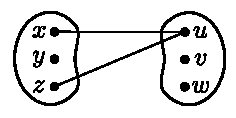
\includegraphics[scale=1]{img/beans/beans1.pdf}
\end{center}
The subset of $S$ being described in this example is $\{(x,u),(z,u)\}$.
Each line joining two dots represents a pair which is being included in the subset of $S$.
For each of the following, provide a picture that describes a subset of $S$ that meets the given specifications.
\begin{enumerate}
\item not a function
\item a function with domain $\{y,z\}$
\item a function with range $\{v\}$
\item a non-function with domain $\{y\}$ and range $\{u,v\}$
\item a function mapping $\{x,y,z\}$ to $\{u,w\}$ which is surjective onto $\{u,w\}$
\item a function mapping $\{x,y,z\}$ to $\{u,w\}$ which is not surjective onto $\{u,w\}$
\item a function mapping $\{x,y\}$ to $\{u,v,w\}$ which is injective
\item a function mapping $\{x,y\}$ to $\{u,v,w\}$ which is not injective
\item a function mapping $\{x,y,z\}$ to $\{u,v,w\}$ which is bijective onto $\{u,v,w\}$ and whose value at $x$ is $w$
\end{enumerate}
}

\ex{Prove that if $X\times Y$ is a function, then either $X\times Y$ must be $\emptyset$ or $Y$ must be a singleton.}



\subsection{Composition and Inverse}
\DEFN{Composite\label{def:comp}}{
$$
S\circ T = 
\COLL{(x,z)}{\EXIST{y}{(x,y)\in T\,\AND\,(y,z)\in S}}.
$$
}

Recall that the right hand side above is a shorthand for
$$
\COLL{p}{\EXIST{x,z}{ p=(x,z) \,\AND\, \EXIST{y}{(x,y)\in T\,\AND\,(y,z)\in S} }}.
$$

\THMNP{Associativity of Composition\label{thm:assoc_comp}}{
$ S\circ (T\circ U) = (S\circ T)\circ U $
}{
$\subseteq$:
Consider any $(x,w)\in S\circ (T\circ U)$.
Get $y$ such that $(x,y)\in T\circ U$ and $(y,w)\in S$.
Since $(x,y)\in T\circ U$, we can also get $z$ such that $(x,z)\in U$ and $(z,y)\in T$.
Now we have found a $y$ satisfying $(z,y)\in T$ and $(y,w)\in S$, so we have shown that $(z,w)\in S\circ T$.
Having found a $z$ such that $(x,z)\in U$ and $(z,w)\in S\circ T$, we conclude that $(x,w)\in (S\circ T)\circ U$.

$\supseteq$:
\putExerciseHeading:
Prove that $(S\circ T)\circ U\subseteq S\circ (T\circ U)$.
}

\THMN{Domain and Range of Composite\label{thm:domran_comp}}{
\begin{enumerate}[(1)]
\item\label{thm:domran_comp1}
If $\ran{T}\subseteq\dom{S}$, then $\dom{S\circ T}=\dom{T}$.
\item\label{thm:domran_comp2}
$\ran{S\circ T}\subseteq \ran{S}$
\end{enumerate}
}
\proofnewline
\textit{Proof of \ref{thm:domran_comp1}}
Assume that $\ran{T}\subseteq\dom{S}$.

$\subseteq$:
Consider any $x\in \dom{S\circ T}$.
Get $z$ such that $(x,z)\in S\circ T$.
Get $y$ such that $(x,y)\in T$ and $(y,z)\in S$.
We have found a $y$ such that $(x,y)\in T$.
It follows that $x\in\dom{T}$.

$\supseteq$:
Consider any $x\in\dom{T}$.
Get $y$ such that $(x,y)\in T$.
Since there exists an $x$ such that $(x,y)\in T$, we have $y\in\ran{T}$.
From our assumption $\ran{T}\subseteq\dom{S}$, it follows that $y\in\dom{S}$.
Get $z$ such that $(y,z)\in S$.
We have found a $y$ such that $(x,y)\in T$ and $(y,z)\in S$.
It follows that $(x,z)\in S\circ T$,
so we have found a $z$ such that $(x,z)\in S\circ T$.
It follows that $x\in \dom{S\circ T}$.
\done
\proofsep
Proving \ref{thm:domran_comp2} is \putExerciseHeading.


\THMN{Essence of Composition\label{thm:ess_comp}}{
\begin{enumerate}[(1)]
\item \label{thm:ess_comp1}
If $f$ and $g$ are functions, then $g\circ f$ is a function and 
$$(g\circ f)(x) = g(f(x)) $$
for all $x\in \dom{g\circ f}$.
\item \label{thm:ess_comp2}
If $f:X\rightarrow Y$ and $g:Y\rightarrow Z$, then $g\circ f:X\rightarrow Z$.
\end{enumerate}
}
\proofnewline
\textit{Proof of \ref{thm:ess_comp1}:}
Assume that $f$ and $g$ are functions.

From Definition \ref{def:comp}, it is clear that every element of $g\circ f$ is a pair.
Thus $g\circ f$ is a set of pairs.

Consider any $x,y,z$ such that $(x,y)$ and $(x,z)$ are in $g\circ f$.
Using the fact that $(x,y)\in g\circ f$,
we can get $a$ such that $(x,a)\in f$ and $(a,y)\in g$.
Using the fact that $(x,z)\in g\circ f$,
we can get $b$ such that $(x,b)\in f$ and $(b,z)\in g$.
Since $(x,a)$ and $(x,b)$ are both in the function $f$, we must have $a=b$.
Since $(a,y)$ and $(b,z)=(a,z)$ are both in the function $g$, we must have $y=z$.

We have argued that $g\circ f$ is a set of pairs, and that whenever $(x,y),(x,z)\in g\circ f$, it follows that $y=z$.
Thus we have shown that $g\circ f$ is a function.

Now consider any $x\in\dom{g\circ f}$.
Get $z$ such that $(x,z)\in g\circ f$.
Get $y$ such that $(x,y)\in f$ and $(y,z)\in g$.
We will now make several uses of Theorem \ref{thm:ess_eval}.
From $(x,y)\in f$ and $(y,z)\in g$, we conclude that $y=f(x)$ and $z=g(y)$.
From $(x,z)\in g\circ f$ (and the just-established fact that $g\circ f$ is a function), we conclude that $z=(g\circ f)(x)$.
Thus we have 
\[
(g\circ f)(x)=z=g(y)=g(f(x)).
\tag*{\qedsymbol}
\]
\proofsep
\textit{Proof of \ref{thm:ess_comp2}:}
Assume that $f:X\rightarrow Y$ and $g:Y\rightarrow Z$.
To show that $g\circ f:X\rightarrow Z$,
we must argue that $g\circ f$ is a function,
that its domain is $X$,
and that it's range is contained in $Z$.
We already know that $g\circ f$ is a function due to part \ref{thm:ess_comp1} and the fact that $f$ and $g$ are functions.

To see that $\dom{g\circ f}=X$, we will use Theorem \ref{thm:domran_comp}.
We have
$$
\ran{f} \subseteq Y = \dom{g},
$$
so part \ref{thm:domran_comp1} of Theorem \ref{thm:domran_comp} applies and we conclude that $\dom{g\circ f}=\dom{f}=X$.

The fact that $\ran{g\circ f}\subseteq Z$ is a consequence
of part \ref{thm:domran_comp2} of Theorem \ref{thm:domran_comp}:
\[
\ran{g\circ f}\subseteq \ran{g} \subseteq Z.
\tag*{\qedsymbol}
\]

The composite $g\circ f$ can be thought of as the function that, when given an input, applies $f$ and then applies $g$.

\ex{Prove that if $S\subseteq A\times B$ and $T\subseteq B\times C$, then $T\circ S\subseteq A\times C$.}

\def\tagA{$(\ast)$}
\def\tagB{$(\ast\ast)$}

\ex{\label{ex:beans2}Let $X=\{x,y,z\}$, 
let $U=\{u,v,w\}$, and let
$A=\{a,b,c,d\}$.
Assume that $x,y,z,u,v,w,a,b,c,d$ are distinct.
In this exercise, we will depict subsets of $X\times U$, $U\times A$, and $X\times A$
in the manner of Exercise \ref{ex:beans1}.
This can give a helpful visual for composition.
Let's do an example.
\indented{
Let $f=\{(x,v),(y,u),(z,v),(z,w)\}$.
Then $f\subseteq X\times U$ and $f$ can be depicted by
\begin{center}
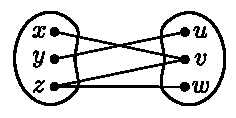
\includegraphics[scale=1]{img/beans/beans2.pdf}
\end{center}
Let $g=\{(u,b),(w,d)\}$.
Then $g\subseteq U\times A$ and $g$ can be depicted by
\begin{center}
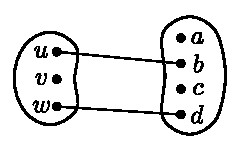
\includegraphics[scale=1]{img/beans/beans3.pdf}
\end{center}
Now $g\circ f\subseteq X\times A$, and we can depict the composition by joining the two pictures together:
\begin{center}
\hfill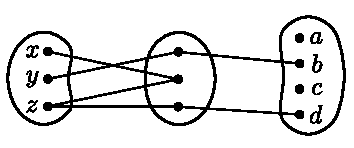
\includegraphics[scale=1]{img/beans/beans4.pdf} \hfill \raisebox{2em}{\tagA}
\end{center}
Then $g\circ f$ can be determined to have the picture
\begin{center}
\hfill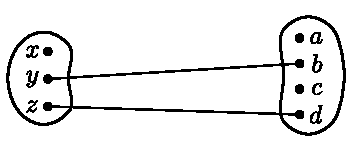
\includegraphics[scale=1]{img/beans/beans5.pdf} \hfill \raisebox{2em}{\tagB}
\end{center}
which is $\{(y,b),(z,d)\}$.
Do you see how to get the picture \tagB{} from \tagA?
}
\begin{enumerate}
\item Prove that if $f$ and $g$ are defined as in the example just given, then $\{(y,b),(z,d)\}\subseteq g\circ f$.
No pictures allowed-- give a real proof.
You can also prove the reverse inclusion if you want, but it's... less fun.
\item For each $f$ and $g$ below, determine $g\circ f$ by producing images like \tagA{} and \tagB.
Your answer for each part below should include an image like \tagA{}, an image like \tagB{}, and a
list of pairs that describes $g\circ f$.
\begin{enumerate}
\item $f=\{
(x,u),(y,v),(z,w)
\}$ and $g=\{
(u,c),(v,a),(w,c)
\}$
\item $f=\{
(x,v),(y,v),(z,v)
\}$ and $g=\{
(u,a),(v,b),(w,d),(v,c)
\}$
\item $f=\{
(x,u),(y,w),(z,v)
\}$ and $g=\{
(v,b),(w,d)
\}$
\item $f=\{
(x,v),(y,v),(z,v)
\}$ and $g=\{
(u,c),(w,c)
\}$
\end{enumerate}
\end{enumerate}
}

\vspace{3em}


\DEFN{Identity Function}{
The \emph{identity function on $A$} is denoted by $\id{A}$ and defined by
$$
\id{A}=\COLL{(x,x)}{x\in A}.
$$
}

Note that the right hand side above is short for
$$
\COLL{p}{\EXIST{x}{p=(x,x)\,\AND\, x\in A}}.
$$

\THMNP{Facts about $\id{A}$\label{thm:ess_id}}{
\begin{enumerate}[(1)]
\item \label{thm:ess_id1} $\id{A}:A\rightarrow A$.
\item \label{thm:ess_id2} $\id{A}(x)=x$ for all $x\in A$.
\item \label{thm:ess_id3} If $f:A\rightarrow B$, then $f\circ \id{A}=f$.
\item \label{thm:ess_id4} If $g:B\rightarrow A$, then $\id{A}\circ g = g$.
\end{enumerate}
}{
Proving \ref{thm:ess_id1}, \ref{thm:ess_id2}, and \ref{thm:ess_id3} is \putExerciseHeading.
We prove \ref{thm:ess_id4} here.

Assume that $g:B\rightarrow A$.
Since $\id{A}:A\rightarrow A$ by part \ref{thm:ess_id1}, 
we have $\id{A}\circ g:B\rightarrow A$ (Theorem \ref{thm:ess_comp} part \ref{thm:ess_comp2}).
In particular, the functions $\id{A}\circ g$ and $g$ have the same domain, $B$.
For any $x\in B$, we have
$$
\begin{array}{lll}
(\id{A}\circ g)(x) & = \id{A}(g(x))  \hspace{3em} &\text{(Theorem \ref{thm:ess_comp} part \ref{thm:ess_comp1})} \\
 & = g(x). &  \text{(part \ref{thm:ess_id2} of this theorem)} 
\end{array}
$$
It follows from Theorem \ref{thm:fn_eq} that $\id{A}\circ g=g$.
}

\DEFN{Reverse\label{def:rev}}{
The \emph{reverse} of $S$ is denoted by $\rev{S}$ and defined by
$$
\rev{S}=\COLL{(y,x)}{(x,y)\in S}.
$$
}

Note that the right hand side above is short for
$$
\COLL{p}{\EXIST{x,y}{p=(y,x)\,\AND\, (x,y)\in S}}.
$$

\THMNP{Essence of Reversal\label{thm:ess_rev}}{
$(x,y)\in S \DARR (y,x)\in \rev{S}.$
}{
$\Rightarrow$:
Assume that $(x,y)\in S$.
We want to prove that $(y,x)\in\rev{S}$.
This seems obvious but let us do it very carefully to avoid confusion.
The proposition $(y,x)\in\rev{S}$ is equivalent to 
\[ \EXIST{a,b}{(y,x)=(b,a)\,\AND\, (a,b)\in S}. \label{eqn:ess_rev}\tag{$\ast$}\]
Letting $b=y$ and $a=x$, we get $(y,x)=(b,a)$ and $(a,b)=(x,y)\in S$.
We conclude (by an \hyperlink{hl:EG}{EG}) that the condition (\ref{eqn:ess_rev}) holds
and therefore that $(y,x)\in\rev{S}$.


$\Leftarrow$:
Assume that $(y,x)\in \rev{S}$.
Get $a$ and $b$ such that $(y,x)=(b,a)$ and $(a,b)\in S$
(carefully check that this is a correct use of Definition \ref{def:rev}).
Then $y=b$ and $x=a$, so $(x,y)\in S$.
}


\THMNP{Double Reversal\label{thm:double_rev}}{
If $S$ is a set of pairs, then
$$
\drev{S}=S.
$$
}{
Assume that $S$ is a set of pairs.
We will make several uses of Theorem \ref{thm:ess_rev}.

$\subseteq$:
Consider any $(x,y)\in\drev{S}$.
It follows that $(y,x)\in\rev{S}$, and from this it follows that $(x,y)\in S$.

$\supseteq$:
Consider any $(x,y)\in S$.
It follows that $(y,x)\in\rev{S}$, and from this it follows that $(x,y)\in \drev{S}$.
}

\ex{
Why is the assumption that $S$ is a set of pairs needed in Theorem \ref{thm:double_rev}?
Exactly what step of the proof would be in error if we did not have this assumption?
}

\THMNP{Reversal, Domain, and Range\label{thm:rev_domran}}{
\begin{enumerate}[(1)]
\item \label{thm:rev_domran1}
$\dom{\rev{S}}=\ran{S}$.
\item \label{thm:rev_domran2}
$\ran{\rev{S}}=\dom{S}$.
\end{enumerate}
}{
Proving \ref{thm:rev_domran2} is \putExerciseHeading.
We prove \ref{thm:rev_domran1} here.

$\subseteq$:
Consider any $z\in \dom{\rev{S}}$.
Get $a$ such that $(z,a)\in\rev{S}$.
Then $(a,z)\in S$.
It follows that $z\in\ran{S}$.

$\supseteq$:
Consider any $z\in\ran{S}$.
Get $a$ such that $(a,z)\in S$.
Then $(z,a)\in\rev{S}$.
It follows that $z\in\dom{\rev{S}}$.
}

\THMNP{Reversal and Composition\label{thm:rev_comp}}{$\rev{(S\circ T)}=\rev{T}\circ\rev{S}$.}{
Proving that $\rev{(S\circ T)}\subseteq\rev{T}\circ\rev{S}$ is \putExerciseHeading.

We will prove that $\rev{T}\circ\rev{S}\subseteq\rev{(S\circ T)}$.
Consider any $(z,w)\in \rev{T}\circ\rev{S}$.
Get $a$ such that $(z,a)\in\rev{S}$ and $(a,w)\in\rev{T}$.
Then we have $(w,a)\in T$ and $(a,z)\in S$.
It follows that $(w,z)\in S\circ T$,
and from this it follows that $(z,w)\in\rev{(S\circ T)}$.
}

\DEFN{Invertibility}{
If $f$ is a function, then 
$f$ is said to be \emph{invertible} if and only if $\rev{f}$ is also a function.
In this context, we will refer to $\rev{f}$ as \emph{the inverse} of $f$.
}

\THMNP{Invertibility of Injections\label{thm:inj_inv}}{If $f$ is a function, then $\rev{f}$ is a function if and only if $f$ is injective.}{
Assume that $f$ is a function.

Suppose that $\rev{f}$ is a function. 
We will use the criterion given in Theorem \ref{thm:inj_xyz} to demonstrate that $f$ is injective.
%Consider any $x,y\in\dom{f}$ such that $f(x)=f(y)$.
Consider any $x,y,z$ such that $(x,y),(z,y)\in f$.
By Theorem \ref{thm:ess_rev}, we have $(y,x),(y,z)\in \rev{f}$.
Since $\rev{f}$ is a function, it follows that $x=z$.
Thus we have proven that $f$ is injective.

Conversely, suppose that $f$ is injective.
It is clear from Definition \ref{def:rev} that $\rev{f}$ is a set of pairs.
To see that $\rev{f}$ is a function, suppose that $(x,y),(x,z)\in\rev{f}$.
By Theorem \ref{thm:ess_rev}, we have $(y,x),(z,x)\in f$.
By Theorem \ref{thm:inj_xyz} and the fact that $f$ is injective, it follows that $y=z$.
Thus we have proven that $\rev{f}$ is a function.
}

Note the role of the word ``conversely'' when it is used to introduce a paragraph.
It serves to separate the ``$\Rightarrow$'' and ``$\Leftarrow$'' portions of the proof.

\THMPL{If $f:X\rightarrow Y$ and $f$ is injective, then $\rev{f}:\ran{f}\rightarrow X$.}{
\putExerciseHeading.
}{\label{thm:inj_inv2}}

\THMPL{If $f$ is an invertible function, $x\in\dom{f}$, and $y\in\ran{f}$, then
$$
f(x)=y\ \DARR\ x=\rev{f}(y)
$$}{
Assume that $f$ is an invertible function, $x\in\dom{f}$, and $y\in\ran{f}$.
Theorem \ref{thm:inj_inv2} tells us that $\ran{f}=\dom{\rev{f}}$, so $y\in\dom{\rev{f}}$
and we are in a position to apply Theorem \ref{thm:ess_eval} as follows:
\[\begin{array}{llll}
f(x) = y & \DARR & (x,y)\in f \hspace{1.5em} & \text{(Theorem \ref{thm:ess_eval})} \\
         & \DARR & (y,x)\in \rev{f}          & \text{(Theorem \ref{thm:ess_rev})}  \\
         & \DARR & \rev{f}(y)=x.             & \text{(Theorem \ref{thm:ess_eval})} 
\end{array}\]
}{
\label{thm:inv_equiv}
}


\THMPL{If $f:X\rightarrow Y$ and $f$ is a bijection onto $Y$, then $\rev{f}:Y\rightarrow X$ and $\rev{f}$ is a bijection onto $X$.}{
Assume that $f:X\rightarrow Y$ and $f$ is a bijection onto $Y$.
Since $f$ is injective, Theorem \ref{thm:inj_inv2} tells us that $\rev{f}:\ran{f}\rightarrow X$.
Since $f$ is surjective onto $Y$, we have $\ran{f}=Y$, and so $\rev{f}:Y\rightarrow X$.
It remains for us to argue that $\rev{f}$ is bijective onto $X$.

We know that $\rev{f}$ is surjective onto $X$ because $\ran{\rev{f}}=\dom{f} = X$, by Theorem \ref{thm:rev_domran}.

Finally, we will use Theorem \ref{thm:inj_inv} 
to argue that $\rev{f}$ is injective.
We already know that $\rev{f}$ is a function, and we also know that $\drev{f}$, which is $f$ by Theorem \ref{thm:double_rev}, is a function.
It follows from Theorem \ref{thm:inj_inv} that $\rev{f}$ is injective.
}{
\label{thm:bij_inv}
}

\THMPL{If $f:X\rightarrow Y$ and $f$ is injective, then $\rev{f}\circ f=\id{X}$.}{
Assume that $f:X\rightarrow Y$ and $f$ is injective.
From Theorem \ref{thm:inj_inv2}
we know that $\rev{f}:\ran{f}\rightarrow X$.
To prove that $\rev{f}\circ f=\id{X}$,
we will use Theorem \ref{thm:fn_eq}.
This means we must show that the domains of $\rev{f}\circ f$ and $\id{X}$ are equal, and that
$\rev{f}\circ f$ and $\id{X}$ take the same value on all elements of the common domain.
We have
$\dom{\id{X}}=X=\dom{\rev{f}\circ f}$ by Theorem \ref{thm:ess_id} part \ref{thm:ess_id1} and Theorem \ref{thm:ess_comp} part \ref{thm:ess_comp2}.

Now consider any $x\in X$.
Our basic argument is as follows:
$$
\begin{array}{llll}
(\rev{f}\circ f)(x) & = & \rev{f}(f(x)) \hspace{1.5em} & \text{(Theorem \ref{thm:ess_comp} part \ref{thm:ess_comp1})} \\
                    & = & x                            & \text{(Theorem \ref{thm:inv_equiv})}                         \\
                    & = & \id{X}(x)                    & \text{(Theorem \ref{thm:ess_id} part \ref{thm:ess_id2})}.
\end{array}
$$
However, some comments are needed to justify the middle line.
Applying Theorem \ref{thm:inv_equiv} to $\rev{f}$ gives us
\[\rev{f}(f(x)) = x\ \DARR\ f(x)=\drev{f}(x),\tag{$\ast$}\label{eqn:inj_leftinv}\]
but we should first check that the hypotheses of Theorem \ref{thm:inv_equiv} are satisfied.
Note that $\rev{f}$ is an invertible function because $\drev{f}=f$ is a function.
And note that $f(x)\in \ran{f}=\dom{\rev{f}}$ and $x\in X=\dom{f}=\ran{\rev{f}}$.
Now Theorem \ref{thm:inv_equiv} applies and we have (\ref{eqn:inj_leftinv}).
The right hand side of (\ref{eqn:inj_leftinv}) holds thanks to Theorem \ref{thm:double_rev},
so we have $\rev{f}(f(x)) = x$ and our argument above is justified.

We have now proven that $(\rev{f}\circ f)(x)=\id{X}(x)$ for all $x\in X$. 
By Theorem \ref{thm:fn_eq}, we have proven that $\rev{f}\circ f=\id{X}$.
}{
\label{thm:inj_leftinv}
}

\THMNP{Inverse and Composition\label{thm:inv_comp}}{If $f:X\rightarrow Y$ and $f$ is a bijection onto $Y$, then
\begin{enumerate}[(1)]
\item \label{thm:inv_comp1}
$f\circ\rev{f}=\id{Y}$.
\item \label{thm:inv_comp2}
$\rev{f}\circ f=\id{X}$.
\end{enumerate}
}{
Assume that $f:X\rightarrow Y$ and $f$ is a bijection onto $Y$.

Since $f$ is injective,
part \ref{thm:inv_comp2}
is Theorem \ref{thm:inj_leftinv}.

By Theorem \ref{thm:bij_inv}, we know that $\rev{f}:Y\rightarrow X$ and $\rev{f}$ is a bijection onto $X$.
Since $\rev{f}$ is injective, we may apply Theorem \ref{thm:inj_leftinv}
to conclude that $\drev{f}\circ\rev{f}=\id{Y}$.
Using Theorem \ref{thm:double_rev} to rewrite this as $f\circ\rev{f}=\id{Y}$, we have proven part \ref{thm:inv_comp1}.
}

\THMNP{\label{thm:comp_inj_surj}Composition, Injectivity, and Surjectivity}{

Assume
that $f:X\rightarrow Y$ and $g:Y\rightarrow Z$.
\begin{enumerate}[(1)]
\item If $f$ and $g$ are injective, then $g\circ f$ is injective.
\item If $g\circ f$ is injective, then $f$ is injective.
\item If $f$ is surjective onto $Y$ and $g$ is surjective onto $Z$,
then $g\circ f$ is surjective onto $Z$.
\item If $g\circ f$ is surjective onto $Z$, then $g$ is surjective onto $Z$.
\item If $f$ is bijective onto $Y$ and $g$ is bijective onto $Z$, then $g\circ f$ is bijective onto $Z$.
\end{enumerate}
}{
\putExerciseHeading.
}

The notation ``$f,g:X\rightarrow Y$'' below is short for ``$f:X\rightarrow Y\ \AND\ g:X\rightarrow Y$''.

\THMNP{\label{thm:comp_cancel}Cancellation of Composite}{Assume
that $f,g:X\rightarrow Y$.
\begin{enumerate}[(1)]
\item\label{thm:comp_cancel1}
If $h:Y\rightarrow Z$, $h$ is injective,
and $h\circ f=h\circ g$, then $f=g$.
\item\label{thm:comp_cancel2}
If $h:Z\rightarrow X$, $h$ is surjective onto $X$,
and $f\circ h=g\circ h$, then $f=g$.
\end{enumerate}
}{
Part \ref{thm:comp_cancel1} is \putExerciseHeading.
We prove \ref{thm:comp_cancel2} here.

Assume that
$f,g:X\rightarrow Y$,
$h:Z\rightarrow X$, 
$h$ is surjective onto $X$,
and $f\circ h=g\circ h$.
Since $f$ and $g$ have the same domain $X$, all we need to do is prove that $f(x)=g(x)$ for all $x\in X$.
Then we will be done by Theorem \ref{thm:fn_eq}.

Consider any $x\in X$.
Since $h$ is surjective onto $X$, there is some $z\in Z$ such that $h(z)=x$ (Theorem \ref{thm:surj_exist}).
Note that $\dom{f\circ h}=Z$ (Theorem \ref{thm:ess_comp}), so we may evaluate $f\circ h$ at $z$.
We have
$$
\begin{array}{llll}
f(h(z)) & = & (f\circ h)(z) \hspace{1.5em} & \text{(Theorem \ref{thm:ess_comp})} \\
        & = & (g\circ h)(z)                & \text{(since $f\circ h=g\circ h$)}  \\
        & = & g(h(z))                      & \text{(Theorem \ref{thm:ess_comp})} .
\end{array}
$$
That is, $f(x)=g(x)$.
} 

Theorem \ref{thm:comp_cancel}
says that injective functions can be cancelled when they are on the left side of a composition,
and surjective functions can be cancelled when they are on the right.
These properties actually \emph{characterize} injectivity and surjectivity.
That is, a function is injective if and only if it is left-cancellable, and it is surjective if and only if it is right-cancellable.
Proving this is \putExerciseHeading, which is challenging and skippable.
The precise assertion is this:
If $h:Y\rightarrow Z$, then $h$ is injective iff $h\circ f=h\circ g\ARR f=g$ for all $f,g:X\rightarrow Y$,
and $h$ is surjective onto $Z$ iff $f\circ h=g \circ h \ARR f=g$ for all $f,g:X\rightarrow Y$.

Theorem \ref{thm:inj_leftinv} tells us that injective functions are ``left-invertible.''
Precisely, this means that they can be composed with something on the left to yield a suitable identity function.
What follows is a sort of converse to Theorem \ref{thm:inj_leftinv}.

\THMNP{Left-Invertible Functions\label{thm:leftinv}}{Assume
that $f:X\rightarrow Y$.
If $$\EXIST{g}{g:Y\rightarrow X\ \AND\ g\circ f=\id{X}},$$
then $f$ is injective.
}{
Assume that $f:X\rightarrow Y$ and that there is some $g$ such that $g:Y\rightarrow X$ and $g\circ f=\id{X}$.
Get such a $g$.
Consider any $x,x'\in X$ such that $f(x)=f(x')$.
Then 
$$x=\id{X}(x)=(g\circ f)(x) = g(f(x))=g(f(x'))=(g\circ f)(x')=\id{X}(x')=x'.$$
}

It is pleasing to know that there is a similar result for right-invertibility and surjectivity:

\THMNP{Right-Invertible Functions\label{thm:rightinv}}{Assume
that $f:X\rightarrow Y$.
If $$\EXIST{g}{g:Y\rightarrow X\ \AND\ f\circ g=\id{Y}},$$
then $f$ is surjective onto $Y$.}{
\putExerciseHeading.
}


\ex{\label{ex:beans3}Let
$S=\{x,y,z\}\times\{u,v,w,a\}$.
Assume that $x,y,z,u,v,w,a$ are distinct.
Define the following subsets of $S$:
$$\begin{array}{lll}
h&=&\{
(x,w),(z,w),(y,v)
\}\\
i&=&\{
(x,v),(y,w),(z,a),(y,u)
\}\\
j&=&\{
(x,v),(y,w),(z,a)
\}
\end{array}$$
\begin{enumerate}
\item Depict each of $h,i,j$ using a picture in the manner of Exercise \ref{ex:beans1}.
As an example, here is a depiction of $h$:
\begin{center}
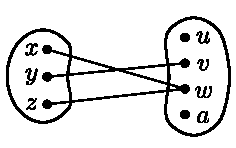
\includegraphics[scale=1]{img/beans/beans7.pdf}
\end{center}
\item One of $h,i,j$ is injective.
Which one?
\item\label{ex:beans3:redo}
For the injection, find a left-inverse.
That is, find a function $g:\{u,v,w,a\}\rightarrow\{x,y,z\}$ such that
$$ g\circ (\text{the injection}) = \id{\{x,y,z\}}. $$
Depict this composition by joining pictures in the manner of Exercise \ref{ex:beans2}.
\item
Redo question \ref{ex:beans3:redo}, but this time find a \emph{different} left-inverse.
\item How many left inverses do you think there are?
\end{enumerate}
}

\ex{\label{ex:beans4}Let
$S=\{x,y,z,a\}\times\{u,v,w\}$.
Assume that $x,y,z,u,v,w,a$ are distinct.
Define the following subsets of $S$:
$$\begin{array}{lll}
h&=&\{
(x,u),(x,v),(y,w),(z,w),(a,w)
\}\\
i&=&\{
(x,u),(y,u),(z,v),(a,w)
\}\\
j&=&\{
(x,u),(y,u),(z,w),(a,w)
\}
\end{array}$$
\begin{enumerate}
\item Depict each of $h,i,j$ using a picture in the manner of Exercise \ref{ex:beans1}.
As an example, here is a depiction of $h$:
\begin{center}
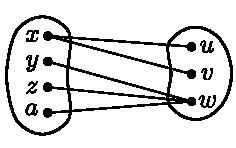
\includegraphics[scale=1]{img/beans/beans6.pdf}
\end{center}
\item One of $h,i,j$ is surjective onto $\{u,v,w\}$.
Which one?
\item\label{ex:beans4:redo}
For the surjection, find a right-inverse.
That is, find a function $g:\{u,v,w\}\rightarrow\{x,y,z,a\}$ such that
$$ (\text{the surjection})\circ g = \id{\{u,v,w\}}. $$
Depict this composition by joining pictures in the manner of Exercise \ref{ex:beans2}.
\item
Redo question \ref{ex:beans4:redo}, but this time find a \emph{different} right-inverse.
\item How many right inverses do you think there are?
\end{enumerate}
}

\vspace{2em}

Theorems \ref{thm:inj_leftinv} and \ref{thm:leftinv} tell us
that left-invertibility is \emph{equivalent} to injectivity.
Theorem \ref{thm:rightinv} tells us that right-invertibility \emph{implies} surjectivity.
You may now be wondering... are surjective functions always right-invertible?

If $f:X\rightarrow Y$ is surjective, then is there some $g:Y\rightarrow X$ such that $f\circ g=\id{Y}$?
Letting $g=\rev{f}$ would not work, because $\rev{f}$ is probably not a function.
If a $g$ is to exist, then how can it be produced?
Imposing various special conditions on $Y$ can make it possible to construct $g$.
However, there is no hope for a general theorem. What is needed for the general statement is an axiom:

\AXIOMN{Axiom of Choice\label{ax:choice}}{If $f:X\rightarrow Y$ and $f$ is surjective onto $Y$, then
there exists a function $g:Y\rightarrow X$ such that $f\circ g=\id{Y}$.
}

We will not use Axiom \ref{ax:choice}, but it is essential for much of modern mathematics.

Putting together Theorems \ref{thm:leftinv} and \ref{thm:rightinv} gives us a nice characterization of bijectivity in terms of composition:

\THMNP{Bijectivity and Isomorphism}{Assume
that $f:X\rightarrow Y$.
Then $f$ is a bijection onto $Y$ if and only if
$$
\EXIST{g}{g:Y\rightarrow X\ \AND\ g\circ f=\id{X}\ \AND\ f\circ g=\id{Y}}.
$$
}{
Assume that $f:X\rightarrow Y$.

If $f$ is a bijection onto $Y$, then letting $g=\rev{f}$ should work due to
Theorems \ref{thm:bij_inv} and \ref{thm:inv_comp}.

Conversely, assume that there exists $g:Y\rightarrow X$
such that $g\circ f=\id{X}$ and $f\circ g=\id{Y}$.
Then there exists $g:Y\rightarrow X$
such that $g\circ f=\id{X}$, so $f$ is injective by Theorem \ref{thm:leftinv}.
And there exists $g:Y\rightarrow X$
such that $f\circ g=\id{Y}$, so $f$ is surjective onto $Y$ by Theorem \ref{thm:rightinv}.
}

\ex{(Challenging)\label{ex:inj_leftinv_real}
Prove that if $f:X\rightarrow Y$, $f$ is injective, and $X$ is nonempty, then there exists
some $g:Y\rightarrow X$ such that $g\circ f=\id{X}$.
(This is what it should really mean for $f$ to be ``left-invertible,'' rather
than what is asserted by Theorem \ref{thm:inj_leftinv}.)
}


\ex{Prove that $\id{\dom{B}}\subseteq \rev{B}\circ B$. Not a thrilling result, but good for practice with definitions.}







\subsection{Image}

\DEFN{Image\label{def:img}}{The
\emph{image of $A$ under $S$} is denoted by $S[A]$ and defined by
$$ S[A]=\COLL{y}{\EXIST{x}{x\in A\,\AND\,(x,y)\in S}}.$$
}

If $S$ is a set of pairs, then $S[A]$
collects together the second entries of all the pairs in $S$ whose first entry is an element of $A$.

\ex{Prove that $S[\dom{S}]=\ran{S}$}

\ex{Prove that $S[\emptyset]=\emptyset$}

\ex{Prove that if $f:X\rightarrow Y$, then $\rev{f}[Y]=X$.}

\vspace{1em}

The set $\rev{f}[B]$ appearing below is often called the \emph{preimage} or the \emph{inverse image} of $B$.

\THMN{Image for Functions\label{thm:img_fn}}{Assume that $f:X\rightarrow Y$.
\begin{enumerate}[(1)]
\item \label{thm:img_fn1}
If $A\subseteq X$, then 
$$f[A]=\COLL{f(a)}{a\in A}.$$
In other words,
$$ y\in f[A]\ \DARR\ \EXIST{a}{y=f(a)\,\AND\,a\in A}. $$
\item \label{thm:img_fn2}
$$\rev{f}[B]=\COLL{x}{x\in X\,\AND\, f(x)\in B}.$$
So if $x\in X$, then
$$ x\in \rev{f}[B]\ \DARR\ f(x)\in B. $$
\end{enumerate}
}

\textit{Proof of \ref{thm:img_fn1}:}
Assume that $f:X\rightarrow Y$ and $A\subseteq X$.

$\subseteq$:
Consider any $z\in f[A]$.
Get $a\in A$ such that $(a,z)\in f$.
By Theorem \ref{thm:ess_eval}, we have $z=f(a)$.
We have shown that there exists an $a\in A$ for which $z=f(a)$,
so $z\in \COLL{f(a)}{a\in A}$.

$\supseteq$:
Consider any $z\in \COLL{f(a)}{a\in A}$.
Get $a\in A$ such that $z=f(a)$.
Observe that $a\in\dom{f}$, since $A\subseteq X$, so we are not breaching into undefined territory!
By Theorem \ref{thm:ess_eval}, we have $(a,z)\in f$.
We have shown that there exists an $a\in A$ for which $(a,z)\in f$,
so $z\in f[A]$.
\done
\proofsep
\textit{Proof of \ref{thm:img_fn2}:}
Assume that $f:X\rightarrow Y$.

$\subseteq$:
Consider any $z\in \rev{f}[B]$.
Get $b\in B$ such that $(b,z)\in\rev{f}$.
Then $(z,b)\in f$.
It follows that $f(z)=b$.
And of course from $(z,b)\in f$ we know that $z\in \dom{f}=X$, so we have
$$z\in\COLL{x}{x\in X\,\AND\, f(x)\in B}.$$

$\supseteq$:
Consider any $z\in X$ such that $f(z)\in B$.
We have $(z,f(z))\in f$,
so $(f(z),z)\in\rev{f}$.
Taking $x=f(z)$, we've shown there exists an $x\in B$ such that $(x,z)\in\rev{f}$.
Therefore $z\in \rev{f}[B]$.
\done

In the context of Theorem \ref{thm:img_fn}, 
where the set of pairs $f$ is a function, it is tempting to refer to $\rev{f}$ as an ``inverse,'' but this would be a terrible mistake.
The set of pairs $\rev{f}$ need not be a function, and so we just refer to it as the ``reverse'' of $f$.


\ex{Prove that if $f:X\rightarrow Y$ and $x\in X$, then $f[\{x\}]=\{f(x)\}$.}

\ex{Prove that if $f:X\rightarrow Y$ and $A\subseteq B\subseteq Y$, then $\rev{f}[A]\subseteq \rev{f}[B]$.}

\ex{Prove that if $f:X\rightarrow Y$ and $A\subseteq B\subseteq X$, then $f[A]\subseteq f[B]$.}

\THMNP{Image and Composition\label{thm:img_comp}}{
$ (g\circ f)[A] = g[f[A]]. $
}{
$\subseteq$:
Consider any $z\in (g\circ f)[A]$.
Get $a\in A$ such that $(a,z)\in g\circ f$.
Get $c$ such that $(a,c)\in f$ and $(c,z)\in g$.
From $a\in A$ and $(a,c)\in f$, it follows that $c\in f[A]$.
From $c\in f[A]$ and $(c,z)\in g$, it follows that $z\in g[f[A]]$.

$\supseteq$:
\putExerciseHeading: Prove that $g[f[A]]\subseteq (g\circ f)[A]$.
}

\ex{Prove that if $f:X\rightarrow Y$, then $f$ is injective
if and only if for all $y\in Y$, $\rev{f}[\{y\}]$ is either empty or it is a singleton.}

\ex{\label{ex:surj_preimage}Prove that if $f:X\rightarrow Y$, then $f$ is surjective onto $Y$ if and only if for all $y\in Y$,
$\rev{f}[\{y\}]$ is nonempty.}

\THMPL{Assume that $f:X\rightarrow Y$, $A\subseteq X$, and $B\subseteq Y$.
\begin{enumerate}[(1)]
\item \label{thm:img_facts1}
$f[\rev{f}[B]]\subseteq B$.
\item \label{thm:img_facts2}
$A\subseteq \rev{f}[f[A]]$.
\item \label{thm:img_facts3}
If $B\subseteq\ran{f}$, then $f[\rev{f}[B]] = B$.
\item \label{thm:img_facts4}
If $f$ is injective, then $\rev{f}[f[A]]=A$.
\end{enumerate}
}{
Proving parts \ref{thm:img_facts1} and \ref{thm:img_facts4} is \putExerciseHeading.
We prove \ref{thm:img_facts2} and \ref{thm:img_facts3}.
We will be relying on the descriptions of image and preimage that are given in Theorem \ref{thm:img_fn}.

To prove \ref{thm:img_facts2}, consider any $a\in A$.
By Theorem \ref{thm:img_fn} part \ref{thm:img_fn1}, we have $f(a)\in f[A]$.
By Theorem \ref{thm:img_fn} part \ref{thm:img_fn2}, it follows that $a\in \rev{f}[f[A]]$.

To prove \ref{thm:img_facts3}, assume that $B\subseteq\ran{f}$.
Note that we have one inclusion from part \ref{thm:img_facts1},
so we only need to prove
that $B\subseteq f[\rev{f}[B]]$.
Consider any $b\in B$.
Then by our assumption we have $b\in\ran{f}$.
Get $x$ such that $(x,b)\in f$. Then $f(x)=b\in B$.
By Theorem \ref{thm:img_fn} part \ref{thm:img_fn2}, the fact that $f(x)\in B$ gives us $x\in \rev{f}[B]$.
By Theorem \ref{thm:img_fn} part \ref{thm:img_fn1}, the fact that $x\in\rev{f}[B]$ gives us $f(x)\in f[\rev{f}[B]]$.
In other words, $b\in f[\rev{f}[B]]$.
}{
\label{thm:img_facts}
}

% INCLUDE THESE LINES IN THMS ONLY VERSION
\newcommand{\preimgNiceLine}[1]{$\rev{f}[A{#1}B]=\rev{f}[A]{#1}\rev{f}[B]$}
% END INCLUDE

\THMNP{Preimage Plays Nice\label{thm:preimg_nice}}{Assume that
$f:X\rightarrow Y$, $A\subseteq Y$, and $B\subseteq Y$.
\begin{enumerate}[(1)]
\item \label{thm:preimg_nice1} \preimgNiceLine{\,\cup\,}
\item \label{thm:preimg_nice2} \preimgNiceLine{\,\cap\,}
\item \label{thm:preimg_nice3} \preimgNiceLine{\,\setminus\,}
\end{enumerate}
}{
Proving \ref{thm:preimg_nice2} and \ref{thm:preimg_nice3} is \putExerciseHeading. We prove \ref{thm:preimg_nice1} here.
Assume that $f:X\rightarrow Y$, $A\subseteq Y$, and $B\subseteq Y$.

$\subseteq$:
Consider any $z\in \rev{f}[A\cup B]$.
Then $z\in X$ and $f(z)\in A\cup B$.
So either $f(z)\in A$ or $f(z)\in B$.

Case 1: If $f(z)\in A$, then $z\in \rev{f}[A]\subseteq  \rev{f}[A]\,\cup\,\rev{f}[B]$.

Case 2: If $f(z)\in B$, then $z\in \rev{f}[B]\subseteq  \rev{f}[A]\,\cup\,\rev{f}[B]$.

$\supseteq$:
Consider any $z\in \rev{f}[A]\,\cup\,\rev{f}[B]$.
Then either $z\in \rev{f}[A]$ or $z\in \rev{f}[B]$.

Case 1: If $z\in \rev{f}[A]$, then $z\in X$ and $f(z)\in A\subseteq A\cup B$, so $z\in \rev{f}[A\cup B]$.

Case 2: If $z\in \rev{f}[B]$, then $z\in X$ and $f(z)\in B\subseteq A\cup B$, so $z\in \rev{f}[A\cup B]$.
}

\ex{Assume that $f:X\rightarrow Y$ and that $A$ and $B$ are subsets of $X$. One of the following two assertions has a proof, while the other does not.
\indented{
$f[A\cup B] = f[A]\,\cup\, f[B]$\\
$f[A\cap B] = f[A]\,\cap\, f[B]$
}
Prove the one that has a proof. You should somehow find yourself blocked from proving the other one. (Open-ended question: What blocks the proof?)}

\ex{
Given any function $f:A\rightarrow B$, let us define an operation ``hat'' as follows:
$$ \widehat{f} = \COLL{(S,f[S])}{S\subseteq A}. $$
\begin{enumerate}
\item Prove that if $f:A\rightarrow B$, then $\widehat{f}:\SUB{A}\rightarrow\SUB{B}$.
\item Prove that if $f:A\rightarrow B$ and $g:B\rightarrow C$, then $\widehat{g\circ f} = \widehat{g}\circ \widehat{f}$.
\end{enumerate}
}

\subsection{Natural Numbers}

Given any term $T$, the string ``$\next{T}$'' forms a term, defined as follows.

\DEFN{Successor}{
$\next{x}=x\cup\{x\}$.
}

We now introduce ten new \hyperlink{hl:constants}{constants} into our language.

\DEFN{\label{def:numbers}Certain Numbers}{
$$
\begin{array}{ll}
0 = \emptyset \hspace{6em} & 5=\next{4} \\
1 = \next{0}  & 6=\next{5} \\
2 = \next{1}  & 7=\next{6} \\
3 = \next{2}  & 8=\next{7} \\
4 = \next{3}  & 9=\next{8} \\
\end{array}
$$
}

\DEFN{Inductive\label{def:ind}}{A
set $J$ is said to be \emph{inductive} if it contains $0$ and it contains $\next{n}$ for every $n$ that it contains.
That is,
$$
\text{$J$ is inductive}\ \DARR\ (0\in J\,\AND\,\ALL{n}{n\in J\ARR\next{n}\in J})
$$
}

We now define the \hyperlink{hl:constants}{constant} $\N$.
Elements of $\N$ are called \emph{natural numbers}.

\DEF{
$\N=\COLL{n}{\ALL{J}{\text{$J$ is inductive}\,\ARR\,n\in J}}$.
}

The set $\N$ of natural numbers can be thought of as the ``smallest'' inductive set:

\THMN{Essence of $\N$\label{thm:ess_N}}{
\begin{enumerate}[(1)]
\item $\N$ is inductive. \label{thm:ess_N1}
\item If $J$ is inductive, then $\N\subseteq J$. \label{thm:ess_N2}
\end{enumerate}
}
\proofnewline
\textit{Proof of \ref{thm:ess_N1}:}
We must show that $0\in\N$ and that 
$\ALL{n}{n\in\N\ARR\next{n}\in\N}$.

Consider any inductive set $J$.
By definition, $0\in J$.
Thus
$\ALL{J}{\text{$J$ is inductive}\,\ARR\,0\in J}$.
In other words, $0\in\N$.

Now we prove that $\ALL{n}{n\in\N\ARR\next{n}\in\N}$.
Consider any $n\in\N$.
Consider any inductive set $J$.
Since $n\in\N$, we know that $n$ is in every inductive set.
In particular, $n\in J$.
Sine $J$ is inductive, it follows that $\next{n}\in J$.
Having shown that $\next{n}\in J$ for an arbitrary inductive $J$,
we conclude that 
$\ALL{J}{\text{$J$ is inductive}\,\ARR\,\next{n}\in J}$.
In other words, $\next{n}\in\N$.
\done
\proofsep
\textit{Proof of \ref{thm:ess_N2}:}
Assume that $J$ is inductive.
Consider any $n\in\N$.
Since $n$ is an element of every inductive set, we have in particular that $n\in J$.
\done


\THMNP{Mathematical Induction\label{thm:ind}}{

If 
$$\SUBST{\pA}{x}{0}$$
and
$$\ALL{n}{n\in\N\ \ARR\ (\SUBST{\pA}{x}{n}\,\ARR\,\SUBST{\pA}{x}{\next{n}})}$$
both hold,
then it follows that
$$
\ALL{n}{n\in\N\,\ARR\,\SUBST{\pA}{x}{n}}.
$$
}{
Assume that $\SUBST{\pA}{x}{0}$ and that $\ALL{n}{n\in\N\ \ARR\ (\SUBST{\pA}{x}{n}\,\ARR\,\SUBST{\pA}{x}{\next{n}})}$.
Define
$$
J=\COLL{x}{(x\in\N)\,\AND\,\pA}.
$$
We argue that $J$ is inductive.

First, we must show that $0\in J$.
This is equivalent to $(0\in\N)\,\AND\,\SUBST{\pA}{x}{0}$.
We know that $0\in\N$ since $\N$ is inductive (Theorem \ref{thm:ess_N} part \ref{thm:ess_N1}).
And we know that $\SUBST{\pA}{x}{0}$ holds because we assumed it.
Therefore we have $0\in J$.

Next, we must show that $\ALL{n}{n\in J\ARR\next{n}\in J}$.
Consider any $n\in J$.
We have $n\in\N$ and $\SUBST{\pA}{x}{n}$.
By our assumption, it follows that $\SUBST{\pA}{x}{\next{n}}$.
Since $\N$ is inductive and $n\in\N$, we have $\next{n}\in\N$.
From
$$
(\next{n}\in\N)\,\AND\,\SUBST{\pA}{x}{\next{n}}
$$
we see that $\next{n}\in J$.
Thus we have established that $J$ is inductive.

By Theorem \ref{thm:ess_N} part \ref{thm:ess_N2}, it follows that $\N\subseteq J$.
So
$$
\ALL{n}{n\in \N\ARR n\in J}.
$$
Since $n\in J$ is equivalent to $(n\in\N)\AND\SUBST{\pA}{x}{n}$,
this proves our theorem.
}

\paragraph{Induction}
Theorem \ref{thm:ind} is often used to prove things about natural numbers.
The technique is called \emph{mathematical induction}.
Suppose you want to prove that all natural numbers are green.
Then you can first prove that $0$ is green; this is called the \emph{base case}.
Then prove that whenever a natural number $n$ is green, it follows that $\next{n}$ is also green;
this is called the \emph{induction step}.
Then mathematical induction allows you to conclude that all natural numbers are green.
Specifically, this would be an application of Theorem \ref{thm:ind} with $\pA$ being ``$x$ is green''.
One says that one is \emph{doing induction on $x$}, since $x$ is the variable that gets replaced by
$0$, $n$, and $\next{n}$ in the application of Theorem \ref{thm:ind}.

To help you with reading and writing proofs that use induction, 
here is a base template applied to the nonsensical ``all natural numbers are green'' example:

\def\BChead{\textit{Base Case:}}
\def\IShead{\textit{Induction Step:}}

\THMMOCK{All natural numbers are green. In other words, $\ALL{n}{n\in\N\ARR\text{$n$ is green}}$.}{
We will prove this by doing induction on $n$ in the proposition ``$n$ is green''.

\BChead{}
\indented{[insert argument convincing reader that $0$ is green]}

\IShead{}
Suppose that $n\in\N$ and $n$ is green.
\indented{[insert argument convincing reader that $\next{n}$ is green]}

By induction (Theorem \ref{thm:ind}), it follows that $\ALL{n}{n\in\N\ARR\text{$n$ is green}}$.
}



\DEFN{Order for $\N$}{
\begin{enumerate}[(1)]
\item $x<y\ \DARR\ x\in y$.
\item $x\leq y\ \DARR\ (x\in y\,\OR\,x=y)$.
\end{enumerate}
}

\THMNP{Essence of Order and Succession\label{thm:ess_ord}}{
\begin{enumerate}[(1)]
\item $x<\next{x}$.
\item $x<\next{y}\ \DARR\ x\leq y$.
\end{enumerate}
}{
\putExerciseHeading.
}


\THMNP{About $0$\label{thm:aboutzero}}{
If $n\in\N$, then
\begin{enumerate}[(1)]
\item $0<\next{n}$.\label{thm:aboutzero1}
\item $0\leq n$.\label{thm:aboutzero2}
\item $0\neq\next{n}$.\label{thm:aboutzero3}
\end{enumerate}
}{
We will prove that $0<\next{n}$ for all $n\in\N$, by doing induction on $n$.

\BChead{}
We have $0<\next{0}$ because it is equivalent to $0\leq 0$.

\IShead{}
Suppose that $n\in\N$ and $0<\next{n}$.
Then $0\leq \next{n}$.
It follows that $0<\next{\next{n}}$.

By induction (Theorem \ref{thm:ind}), we have proven that $0<\next{n}$ for every natural number $n$.
This completes the proof of part \ref{thm:aboutzero1}.

Part \ref{thm:aboutzero2} is equivalent to part \ref{thm:aboutzero1}.

To prove part \ref{thm:aboutzero3}, assume that $n\in\N$ and
Suppose for the sake of contradiction that $0=\next{n}$.
Then it follows from part \ref{thm:aboutzero1} that $0\in 0$.
But $0=\emptyset$ is empty.
}



\THMNP{Predecessor\label{thm:pred}}{If
$n\in\N$ and $n\neq 0$, then $n=\next{m}$ for some $m\in\N$.
}{
We must prove that
\[
\ALL{n}{n\in\N\ARR(n\neq 0\ARR\EXIST{m}{m\in\N\,\AND\,n=\next{m}})}.
\tag{$\ast$}\label{eqn:pred}
\]
We will do this by doing an induction on $n$ in the proposition
$$
n\neq 0\ARR\EXIST{m}{m\in\N\,\AND\,n=\next{m}}.
$$
\BChead{}
It is vacuously true that
$
0\neq 0\ARR\EXIST{m}{m\in\N\,\AND\,0=\next{m}}.
$

\IShead{}
Suppose that $n\in\N$ and $
n\neq 0\ARR\EXIST{m}{m\in\N\,\AND\,n=\next{m}}.
$
We must now show that
$$
\next{n}\neq 0\ARR\EXIST{m}{m\in\N\,\AND\,\next{n}=\next{m}}.
$$
Assume that $\next{n}\neq 0$.
Taking $m=n$ gives $m\in\N$ and $\next{n}=\next{m}$, so
$\EXIST{m}{m\in\N\,\AND\,\next{n}=\next{m}}$. This completes the induction step.

By induction (Theorem \ref{thm:ind}), we have proven (\ref{eqn:pred}).
}



\THMNP{Succession Preserves Order\label{thm:succ_ord}}{Assume that $n\in\N$.
\begin{enumerate}[(1)]
\item\label{thm:succ_ord1} 
If $m<n$, then $\next{m}\leq n$.
\item\label{thm:succ_ord2} 
If $m<n$, then $\next{m}<\next{n}$.
\end{enumerate}
}{
Part \ref{thm:succ_ord2} is equivalent to part \ref{thm:succ_ord1}. We prove part \ref{thm:succ_ord1}.

We will prove
$$m<n\ \ARR\ \next{m}\leq n$$
for all $n\in\N$ by doing induction on $n$.

\BChead{}
Since $\neg(m<0)$, we have
$$m<0\ \ARR\ \next{m}\leq 0$$
and the base case is done.

\IShead{}
Suppose that $n\in\N$ and
\[m<n\ \ARR\ \next{m}\leq n.\label{eqn:succ_ord}\tag{$\ast$}\]
Now assume that $m<\next{n}$; we must prove that $\next{m}\leq\next{n}$.
Our assumption $m<\next{n}$ implies that $m \leq n$.

Case 1: Suppose that $m < n$. Then $\next{m}\leq n$ by the induction hypothesis (\ref{eqn:succ_ord}).
It follows that $\next{m}<\next{n}$, and therefore that $\next{m}\leq\next{n}$.

Case 2: Suppose that $m=n$. Then $\next{m}=\next{n}$, so we again have $\next{m}\leq\next{n}$.
}

Note the use of the words ``induction hypothesis'' to refer to the proposition that was assumed for the sake of establishing an induction step.

\THMNP{Transitivity for Order on $\N$\label{thm:trans_N}}{Assume that $n,m,k\in\N$.
\begin{enumerate}[(1)]
\item \label{thm:trans_N1}
If $n<m$ and $m<k$, then $n<k$.
\item \label{thm:trans_N2}
If $n\leq m$ and $m<k$, then $n<k$.
\item \label{thm:trans_N3}
If $n<m$ and $m\leq k$, then $n<k$.
\item \label{thm:trans_N4}
If $n\leq m$ and $m\leq k$, then $n\leq k$.
\end{enumerate}
}{
Parts \ref{thm:trans_N2}, \ref{thm:trans_N3}, and \ref{thm:trans_N4} follow from part \ref{thm:trans_N1}; showing this
is \putExerciseHeading. We prove \ref{thm:trans_N1} here. Assume that $n,m\in\N$.
We will show that
$$ (n<m\ \AND\ m<k)\ \ARR\ n<k $$
for all $k\in\N$, by doing induction on $k$.

\BChead{}
We have 
$ (n<m\,\AND\,m<0)\,\ARR\,n<0 $ simply because $\neg(m<0)$.

\IShead{}
Suppose that $k\in\N$ and 
$$ (n<m\ \AND\ m<k)\ \ARR\ n<k. $$
We will prove that 
$$ (n<m\ \AND\ m<\next{k})\ \ARR\ n<\next{k}. $$
Assume that $n<m$ and $m<\next{k}$.
Then $m\leq k$.

Case 1: Suppose that $m< k$.
Then we have both $n<m$ and $m<k$, so it follows from the induction hypothesis that $n<k$.

Case 2: Suppose that $m = k$.
Then, since $n<m$, we have $n<k$.

In both cases we obtained $n<k$, so it must be that $n<k$.
It follows that $n\leq k$, and therefore that $n<\next{k}$.
This completes the induction step.
}

\THMPL{If $n < m$ and $m\in\N$, then $n\in\N$.}{
\putExerciseHeading.
Hint: Do an induction on $m$ to prove ``$n < m\ARR n\in\N$'' for all $m\in\N$.
}{
\label{thm:N_closed}
}

\ex{Prove that if $m\in\N$ then $m\subseteq\N$.}

\THMNP{Irreflexivity for Order on $\N$\label{thm:irr_N}}{If $n\in\N$, then $\neg(n<n)$}{
We will use induction to prove that $\ALL{n}{n\in\N\ARR\neg(n<n)}$.

\BChead{}
$\neg(0<0)$ holds because it is equivalent to $\emptyset\notin\emptyset$.

\IShead{}
Suppose that $n\in\N$ and $\neg(n<n)$.
Suppose, for the sake of obtaining a contradiction, that $\next{n}<\next{n}$.
Then $\next{n}\leq n$.

Case 1: If $\next{n}=n$ then $\next{n}<\next{n}$ gives us $n<n$, which contradicts the induction hypothesis.

Case 2: Suppose that $\next{n}< n$.
Then since $n<\next{n}$ and $\next{n}<n$, it follows by transitivity (Theorem \ref{thm:trans_N}) that $n<n$.
This contradicts the induction hypothesis.
}

\ex{\label{ex:NnotinN}Prove that $\N\notin\N$. Hint: There is a very short proof.}

\THMNP{Successor Cancels\label{thm:succ_canc}}{Assume that $n,m\in\N$.
\begin{enumerate}[(1)]
\item\label{thm:succ_canc1}
If $\next{m}<\next{n}$, then $m<n$
\item\label{thm:succ_canc2}
If $\next{m}=\next{n}$, then $m=n$.
\end{enumerate}
}{
Assume that $n,m\in\N$.

To prove \ref{thm:succ_canc1}, assume that $\next{m}<\next{n}$.
Then $\next{m}\leq n$, so we have
$$
m<\next{m}\leq n.
$$
By transitivity (Theorem \ref{thm:trans_N}), it follows that $m<n$.

Now we prove \ref{thm:succ_canc2}.
Assume that $\next{m}=\next{n}$.
Since $m\in\next{m}=\next{n}$, we have $m\leq n$. Similarly, we have $n\leq m$.
We will show that $m\subseteq n$ and $n\subseteq m$.

$\subseteq$:
Consider any $k\in m$.
By Theorem \ref{thm:N_closed}, it follows that $k\in\N$.
We now have $k<m\leq n$ and we may apply transitivity to conclude that $k<n$.
In other words, $k\in n$.

$\supseteq$:
Consider any $k\in n$.
By Theorem \ref{thm:N_closed}, it follows that $k\in\N$.
We now have $k<n\leq m$ and we may apply transitivity to conclude that $k<m$.
In other words, $k\in m$.
}

\THMNP{\label{thm:tri_N}Trichotomy for Order on $\N$}{Assume
that $n,m\in\N$.
Then either $m<n$, $n<m$, or $m=n$,
and only \emph{one} of these conditions holds.
That is,
\begin{enumerate}[(1)]
\item\label{thm:tri_N1}
$(m=n)\ \OR\ (m<n)\ \OR\ (n<m)$.
\item\label{thm:tri_N2}
$\neg(m=n\ \AND\ m<n)$.
\item\label{thm:tri_N3}
$\neg(m=n\ \AND\ n<m)$.
\item\label{thm:tri_N4}
$\neg(m<n\ \AND\ n<m)$.
\end{enumerate}
}{
Assume 
that $m\in\N$.
We will prove that
$$
\ALL{n}{n\in\N\ \ARR\ ((m=n)\ \OR\ (m<n)\ \OR\ (n<m))}
$$
by doing induction on $n$.

\BChead{}
We have 
$$(m=0)\ \OR\ (m<0)\ \OR\ (0<m)$$
because we have $0\leq m$ from Theorem \ref{thm:aboutzero}.

\IShead{}
Suppose that $n\in\N$ and 
$$(m=n)\ \OR\ (m<n)\ \OR\ (n<m).$$
\putExerciseHeading: Complete the proof of \ref{thm:tri_N1} from here
by proving that
$$(m=\next{n})\ \OR\ (m<\next{n})\ \OR\ (\next{n}<m)$$
in each of the three cases.

Proving \ref{thm:tri_N2}, \ref{thm:tri_N3}, and \ref{thm:tri_N4} is \putExerciseHeading.
}

\ex{\label{ex:N_antisymmetry}Prove that if $n,m\in\N$, then $(n\leq m \  \AND\  m\leq n)\ \ARR\ n=m$.}

\ex{Prove that if $n,m\in\N$, then $\neg(n\leq m)\ \DARR\ m<n$.\label{ex:notleq}}

\ex{Prove that $2<5$. Prove that $4 \neq 7$.}

\ex{\label{ex:setminus_decrement}Assume that $n=\next{m}$. Prove that $n\setminus\{m\}=m$.}

\DEFN{Minimum}{Given
$A\subseteq\N$, we say that $n$ \emph{is a minimum of} $A$ if and only if $n\in A$ and
$\ALL{a}{a\in A\ \ARR\ n\leq a}$.
}

\ex{Prove that if a subset $A$ of $\N$ has $n$ and $m$ as minima, then it follows that $n=m$.
This justifies saying ``the minimum of $A$'' rather than ``a minimum of $A$,'' when a minimum is known to exist.}

\ex{Assume that $A\subseteq \N$. To say that $A$ has a minimum is to say
that $\EXIST{n}{n\in A\ \AND\ \ALL{a}{a\in A\ARR n\leq a}}$.
Write down what it means for $A$ to \emph{not} have a minimum.
Do this by \hyperlink{hl:NOTUSE}{pushing} the negation in all the way and applying the result from Exercise \ref{ex:notleq}.}


\THMNP{Well-Ordering of $\N$\label{thm:wellord}}{Every
nonempty  set of natural numbers has a minimum. That is, if $A\subseteq\N$ then
$$
A\neq \emptyset \ARR \EXIST{n}{n\in A\ \AND\ \ALL{a}{a\in A\ARR n\leq a}}.
$$
}{
Assume that $A\subseteq \N$. We will prove the contrapositive of the theorem:
if $A$ does not have a minimum, then $A$ must be empty. 
Assume that $A$ does not have a minimum.

We will now do an induction on $k$ to prove that
\[
\ALL{m}{(m\in\N\ \AND\ m\leq k)\ \ARR\ m\notin A}
\label{eq:wellord}\tag{$\ast$}\]
for all $k\in\N$. Then we will be done, as you will check in the following exercise.

\putExerciseHeading: Prove that if (\ref{eq:wellord}) holds for all $k\in\N$, then $A$ is empty.

\BChead{}
We must show that
$$ \ALL{m}{(m\in\N\ \AND\ m\leq 0)\ \ARR\ m\notin A}. $$
Consider any $m\in\N$ such that $m\leq 0$.
Suppose, for the sake of contradiction, that $m\in A$.
Consider any $a\in A$. We have $0\leq a$ by Theorem \ref{thm:aboutzero}.
From $m\leq 0 \leq a$ we get $m\leq a$.
Since $a$ is an arbitrary element of $A$, we have shown that $\ALL{a}{a\in A\ARR m\leq a}$.
In other words, $m$ is a minimum of $A$. This contradicts our assumption that $A$ has no minimum.

\IShead{}
Suppose that 
$$ \ALL{m}{(m\in\N\ \AND\ m\leq k)\ \ARR\ m\notin A}. $$
We must show that 
$$ \ALL{m}{(m\in\N\ \AND\ m\leq \next{k})\ \ARR\ m\notin A}. $$
Consider any $m\in\N$ such that $m\leq \next{k}$.
Suppose, for the sake of contradiction, that $m\in A$.
Consider any $a\in A$.
By the induction hypothesis, we have $a\leq k\ARR a\notin A$.
Therefore we must have $\neg(a\leq k)$.
By trichotomy (Theorem \ref{thm:tri_N}), it follows that $k<a$ (see also Exercise \ref{ex:notleq}).
By Theorem \ref{thm:succ_ord}, we obtain $\next{k}\leq a$.
From $m\leq\next{k}\leq a$ we get $m\leq a$.
Since $a$ is an arbitrary element of $A$, we
have shown that $\ALL{a}{a\in A\ARR m\leq a}$.
In other words, $m$ is a minimum of $A$. This contradicts our assumption that $A$ has no minimum. 
}

\ex{(Open-ended) Why did (\ref{eq:wellord}) have to be so complicated in the proof of Theorem \ref{thm:wellord}?
Why couldn't it just have been ``$k\notin A$''? Try carrying out the proof with (\ref{eq:wellord})
replaced by ``$k\notin A$'' and observe what blocks the proof from working.}

The well-ordering theorem, Theorem \ref{thm:wellord}, provides a new and sometimes more powerful way to carry out a proof by induction.
Suppose you want to prove that all natural numbers are green. Then instead of proving a base case and an induction step, you can frame
your argument like this:

\THMMOCK{All natural numbers are green.}{
Define $A$ to be the set of non-green natural numbers.
Suppose, for the sake of contradiction, that $A$ is nonempty.
Then by well-ordering (Theorem \ref{thm:wellord}), there is a minimum element $n$ of $A$.
That is, there is a minimum non-green natural number $n$.
\indented{[insert argument convincing reader that there exists $m<n$ such that $m$ is non-green]}
The fact that $m<n$ and $m\in A$ contradicts that $n$ was the minimum of $A$.
}

%\ex{ Assume that $J$ is an inductive set. We know from Theorem \ref{thm:ess_N} that $\N\subseteq J$. Prove that $\N\subseteq J$ from well-ordering only.
%}


\subsection{Recursion}

A function $f:\N\rightarrow X$ whose domain is $\N$ is called a \emph{sequence}.
Sequences are sometimes described by listing the first few outputs in order, and then putting ``\ldots''.
Here is an example:
$$
f(0)=2,\ f(1)=3,\ f(2)=4,\ f(3)=5,\ \ldots
$$
In this example, it seems that $f:\N\rightarrow\N$, and we can guess what $f$ is intended to be.
We can guess that the ``\ldots'' are trying to communicate that
$f(n)=\next{\next{n}}$ for all $n\in\N$, or in other words that
$f=\COLL{(n,\next{\next{n}})}{n\in\N}$. It might
be better to just define $f$ explicitly like this,
rather than create unnecessary guessing with ``\ldots''.

Now consider the following example
$$
f(0)=2,\ 
f(1)=4,\ 
f(2)=6,\ 
f(3)=8,\ 
\ldots 
$$
Now what in the world is $f$ supposed to be? What is ``\ldots'' trying to communicate here?
You might want to write something like ``$f(n)=2\cdot n+2$'',
but ``$+$'' and ``$\cdot$'' have yet to be defined! 
The sort of pattern we \emph{can} describe with the machinery built so far is that
$f(\next{n})$ seems to always equal $\next{\next{f(n)}}$.
That is, we can describe the output of $f$ in terms of ``previous'' outputs.
This is called a \emph{recursion rule}.
The list of outputs above is an attempt to communicate that $f$ has the following two properties:
\begin{itemize}
\item $f(0)=2$. 
\item $\ALL{n}{n\in\N\ \ARR\ f(\next{n})=\next{\next{f(n)}}}$
\end{itemize}
Still, how is $f$ \emph{defined} exactly?
The recursion rule is just some property that $f$ is asserted to satisfy--
how do we know that there even \emph{is} a function satisfying that property?
The following theorems are concerned with resolving this issue.

\THMNP{Definition by Recursion - Existence\label{thm:rec_exist}}{

If $s\in X$ and $r:X\rightarrow X$, then there exists an $f:\N\rightarrow X$ such that
$f(0)=s$ and
$$ \ALL{n}{n\in\N\ \ARR\ f(\next{n})=r(f(n)) }. $$
}{
Assume that $s\in X$ and $r:X\rightarrow X$. Define
$$
Z=\COLL{h}{h\subseteq\N\times X\ \ \AND\ \ (0,s)\in h\ \ \AND\ \ \ALL{n,x}{(n,x)\in h\ \ARR\ (\next{n},r(x))\in h}}.
$$
The set $Z$ can be thought of as collecting together all the sets of pairs that sort of have the properties that we want,
except that they might contain more elements than they need in order to do so.
For example, it is easy to see that $\N\times X$ is an element of $Z$.
The main problem with elements of $Z$ is that most of them are not functions.
However, if we attempt to collect only the ``essential'' pairs that every element of $Z$ must have in order to be an element of $Z$,
then we may find that we have a function that has the desired properties. Define
$$
f=\COLL{p}{\ALL{h}{h\in Z\ARR p\in h}}.
$$
Since $\N\times X\in Z$, we have $p\in f\,\ARR\,p\in \N\times X$ for all $p$, so $f\subseteq\N\times X$.
Since we have $f\subseteq\N\times X$, if we want to prove that $f:\N\rightarrow X$ then we only need to show that $f$ is a function and $\N\subseteq\dom{f}$
(see Theorem \ref{thm:mapping_convenience}).
To finish the proof of this theorem, then, we need to prove the following claims:
\begin{enumerate}[(1)]
\item $\N\subseteq\dom{f}$. \label{claim:rec_exist_1}
\item $f$ is a function. \label{claim:rec_exist_2}
\item $f(0)=s$. \label{claim:rec_exist_3}
\item $ \ALL{n}{n\in\N\ \ARR\ f(\next{n})=r(f(n)) }. $ \label{claim:rec_exist_4}
\end{enumerate}
To do this, we will first prove some helper claims:
\begin{enumerate}[(1),resume]
\item $f\in Z$. \label{claim:rec_exist_5}
\item $(0,s)\in f$ and $s$ is unique with respect to this property. That is, $\COLL{x}{(0,x)\in f}=\{s\}$.\label{claim:rec_exist_6}
\end{enumerate}
\textit{Proof of Claim \ref{claim:rec_exist_5}:}
We now argue that $f\in Z$.
We already have $f\subseteq\N\times X$.
We have $(0,s)\in f$ because whenever $h\in Z$, it follows that $(0,s)\in h$.
Now consider any $(n,x)\in f$. We must show that $(\next{n},r(x))\in f$.
Consider any $h\in Z$. Since $(n,x)\in f$, we have $(n,x)\in h$.
It follows that $(\next{n},r(x))\in h$, because $h\in Z$.
Since we have shown that $(\next{n},r(x))\in h$ for all $h\in Z$, we have shown that $(\next{n},r(x))\in f$.
Thus we have shown that $f\in Z$.

\textit{Skippable Comment:} It is easy to see from the construction of $f$ that $f\subseteq h$ for every $h\in Z$.
So $f$ is an element of $Z$ which is a subset of every element of $Z$. Thus $f$ can be thought of as the ``smallest''
set of pairs in $Z$.

\textit{Proof of Claim \ref{claim:rec_exist_6}:}
We already have that $(0,s)\in f$ from Claim \ref{claim:rec_exist_5},
so we only need to prove here that $s$ is unique.
Suppose that $(0,x)\in f$, and suppose for the sake of contradiction that $x\neq s$.
Define $g=f\setminus\{(0,x)\}$.

\putExerciseHeading: Prove that $g\in Z$. 

Since $(0,x)\in f$ and $g\in Z$, we should have $(0,x)\in g$. We have arrived at a contradiction, so Claim \ref{claim:rec_exist_6} is proven.


\textit{Proof of Claim \ref{claim:rec_exist_1}:}
We will do induction on $n$ to prove that $\ALL{n}{n\in\N\,\ARR\, n\in\dom{f}}$.

\BChead{}
Since $(0,s)\in f$, we have $0\in\dom{f}$.

\IShead{}
Suppose that $n\in\N$ and $n\in\dom{f}$.
Get $x$ such that $(n,x)\in f$.
Since $f\in Z$, it follows that $(\next{n},r(x))\in f$.
Therefore $\next{n}\in\dom{f}$.

By induction, Claim \ref{claim:rec_exist_1} is proven.

\textit{Proof of Claim \ref{claim:rec_exist_2}:}
Since $f\subseteq \N\times X$, we know that $f$ is a set of pairs. We must prove that
$$
\ALL{x,y,z}{(x,y),(x,z)\in f\ \ARR\ y=z}.
$$
This is equivalent to
$$
\ALL{n}{n\in\N\ \ARR\ \ALL{x,y}{(n,x),(n,y)\in f\ \ARR\ x=y}},
$$
which we will prove by doing induction on $n$.

\BChead{}
Suppose that $(0,x),(0,y)\in f$. Then by Claim \ref{claim:rec_exist_6} we have $x=s=y$.

\IShead{}
Suppose that $n\in\N$ and that $(n,x),(n,y)\in f\,\ARR\, x=y$ for all $x,y$.
Consider any $x,y$ such that $(\next{n},x),(\next{n},y)\in f$.
By Claim \ref{claim:rec_exist_1}, we can get $z$ such that $(n,z)\in f$.
We will argue that $x=r(z)=y$.

Suppose, for the sake of contradiction, that $x\neq r(z)$.
Define $g=f\setminus\{(\next{n},x)\}$.
\indented{Subclaim: $g\in Z$.\\
\textit{Proof of Subclaim:}
Since $g\subseteq f\subseteq\N\times X$, we have $g\subseteq \N\times X$.
We know that $(0,s)\in f$ from Claim \ref{claim:rec_exist_6}, and it cannot be that $(0,s)=(\next{n},x)$
because it cannot be that $0=\next{n}$ (see Theorem \ref{thm:aboutzero}).
Therefore $(0,s)\in g$.
Now we must show that $\ALL{n,x}{(n,x)\in g\ \ARR\ (\next{n},r(x))\in g}$.
Consider any $(m,w)\in g$.
Since $f\in Z$ and $(m,w)\in f$, we have $(\next{m},r(w))\in f$.
In order to deduce $(\next{m},r(w))\in g$, we need to ensure that $(\next{m},r(w))$
is not equal to $(\next{n},x)$.
Suppose, for the sake of contradiction, that $(\next{m},r(w))=(\next{n},x)$.
Then $\next{m}=\next{n}$ and $r(w)=x$.
By Theorem \ref{thm:succ_canc}, it follows that $m=n$. Then our induction hypothesis applies to 
the situation $(n,z),(m,w)\in f$ and tells us that $z=w$.
Thus $x=r(w)=r(z)$, contradicting our assumption that $x\neq r(z)$.
This proves the subclaim.
}%
Since $(\next{n},x)\in f$ and $g\in Z$, we should have $(\next{n},x)\in g$. We have arrived
at a contradiction, and so we conclude that $x=r(z)$.

The same argument can be applied to $y$ show that $y=r(z)$.
Therefore $x=y$, and the induction step is complete.

By induction, Claim \ref{claim:rec_exist_2} is proven.

Claim \ref{claim:rec_exist_3} immediately follows from the fact that $f$ is a function and $(0,s)\in f$.



\textit{Proof of Claim \ref{claim:rec_exist_4}:}
Consider any $n\in\N$.
Then $n\in\dom{f}$, so $(n,f(n))\in f$. 
Since $f\in Z$, it follows that $(\next{n},r(f(n)))\in f$.
Therefore, since $f$ is a function, we have $f(\next{n})=r(f(n))$.
}

\THMN{Definition by Recursion - Uniqueness\label{thm:rec_unique}}{

Assume that $s\in X$ and $r:X\rightarrow X$. If
\begin{enumerate}[(1)]
\item \label{hyp:rec_unique1}
$f,g:\N\rightarrow X$,
\item \label{hyp:rec_unique2}
$f(0)=g(0)=s$,
\item \label{hyp:rec_unique3}
$\ALL{n,x}{n\in\N\ARR f(\next{n})=r(f(n))}$, and
\item \label{hyp:rec_unique4}
$\ALL{n,x}{n\in\N\ARR g(\next{n})=r(g(n))}$,
\end{enumerate}
then $f=g$.
}
\proofnewline
\textit{Proof:}
Assume that $s\in X$,
$r:X\rightarrow X$,
and \ref{hyp:rec_unique1}-\ref{hyp:rec_unique4} hold.
By Theorem \ref{thm:fn_eq}, if we prove that 
$$ \ALL{n}{n\in\N\ \ARR\ f(n)=g(n)} $$
then we will have $f=g$.
We proceed with an induction on $n$.

\BChead{}
The base case $f(0)=g(0)$ is built into assumption \ref{hyp:rec_unique2}.

\IShead{}
Suppose that $n\in\N$ and $f(n)=g(n)$.
Then
\[
f(\next{n})=r(f(n))=r(g(n))=g(\next{n}).
\tag*{\qedsymbol}
\]

We now have the ability to define a function (with domain $\N$) by specifying its value at $0$ and specifying a recursion rule.

\ex{\label{ex:recursion01}
Define $r:\N\rightarrow\N$ by $r(n)=\next{\next{n}}$.
Let $f:\N\rightarrow\N$ be the unique function that satisfies $f(0)=2$ and $f(\next{n})=r(f(n))$
for all $n\in\N$.
\begin{enumerate}
\item Prove that $f(3)=8$.
\item Prove that $2\leq f(n)$ for all $n\in\N$.
\end{enumerate}
}

\ex{
Define $r$ and $f$ as in Exercise \ref{ex:recursion01}.
Assume that $x\neq y$. Define $r'=\{(x,y),(y,x)\}$.
Let $g:\N\rightarrow \{x,y\}$ be the unique function that satisfies
$g(0)=x$ and $g(\next{n})=r'(g(n))$.
\begin{enumerate}
\item Prove that $r':\{x,y\}\rightarrow\{x,y\}$ and $r'$ is a bijection onto $\{x,y\}$.
\item Prove that $r'\circ r'=\id{\{x,y\}}$
\item Prove that $g(3)=y$.
\item Prove that $g(f(n))=x$ for all $n\in\N$.
\end{enumerate}
}


\subsection{Addition}

\DEFN{Adding One\label{def:addone}}{
$\addone=\COLL{(n,\next{n})}{n\in\N}$.
}

\ex{
\begin{enumerate}
\item
Prove that $\addone:\N\rightarrow\N$.
\item
Prove that $\addone$ is injective
\item
Prove that $\addone$ is not surjective onto $\N$.
\end{enumerate}
}

\DEFN{Adding $n$\label{def:addn}}{
Define $\add:\N\rightarrow\COLL{f}{f:\N\rightarrow\N}$
to be the unique function that satisfies
\begin{itemize}
\item $\add(0)=\id{\N}$ \ \ and
\item $\add(\next{n})=\addone\circ (\add(n))$ \ \ for all $n\in\N$.
\end{itemize}
}

\ex{The
definition above is using Theorems
\ref{thm:rec_exist}
and
\ref{thm:rec_unique},
but some hypotheses need to be verified in order for those theorems to apply.
Let $X=\COLL{f}{f:\N\rightarrow\N}$.
Define the recursion rule that is being used in Definition \ref{def:addn}.
That is, define the function that plays the role of ``$r$''
in Theorem \ref{thm:rec_exist}.
Prove that the $r$ that you define satisfies $r:X\rightarrow X$.
}

\ex{
\begin{enumerate}
\item Prove that $\add(3)=\addone\circ(\addone\circ\addone)$.
\item Prove that $\add(3)(2)=5$.
\end{enumerate}
}

\DEFN{Addition\label{def:plus}}{ Assume that $a,b\in\N$. Then we define
$$
a+b = \add(b)(a).
$$
}

\ex{
\begin{enumerate}
\item Prove that $1+1=2$.
\item Prove that $2+3=5$.
\item Prove that $3+2=5$.
\end{enumerate}
}

\THMNP{Essence of $+$\label{thm:ess_plus}}{
Assume that $m,n\in\N$. Then
\begin{enumerate}[(1)]
\item\label{thm:ess_plus1} $m+n\in\N$.
\item\label{thm:ess_plus2} $m+0 = m$.
\item\label{thm:ess_plus3} $m+\next{n}=\next{m+n}$.
\item\label{thm:ess_plus4} $\next{n}=n+1$.
\item\label{thm:ess_plus5} $m+(n+1)=(m+n)+1$.
\end{enumerate}
}{
\putExerciseHeading.
}

From now on, whenever $n\in\N$ we may use ``$\next{n}$'' and ``$n+1$'' interchangeably.

\THMN{Properties of $+$\label{thm:prop_plus}}{Assume
that $m,n,k\in\N$. Then\\[-0.5em]
\begin{enumerate}[(1)]
\item\label{thm:prop_plus1}
$ m+(n+k) = (m+n)+k $
\hfill (associativity for $+$)
\item\label{thm:prop_plus2}
$ n+0=n $
\hfill ($0$ is a right-identity for $+$)
\item\label{thm:prop_plus3}
$ 0+n=n $
\hfill ($0$ is a left-identity for $+$)
\item\label{thm:prop_plus4}
$ 1+n=n+1 $
\hfill (preliminary to commutativity)
\item\label{thm:prop_plus5}
$ m+n=n+m $
\hfill (commutativity for $+$)
\item\label{thm:prop_plus6}
$ m<n\ \ARR\ m+k<n+k $
\hfill ($+$ respects $<$)
\item\label{thm:prop_plus7}
$ m+k=n+k\ \ARR\ m=n $
\hfill ($+$ cancels under $=$)
\item\label{thm:prop_plus8}
$ m+k<n+k\ \ARR\ m<n $
\hfill ($+$ cancels under $<$)
\item\label{thm:prop_plus9}
$ m+n=0\ \ARR\ (m=0\,\AND\,n=0) $
\item\label{thm:prop_plus10}
$ m+n=1\ \ARR\ ((m=1\,\AND\, n=0)\,\OR\,(m=0\,\AND\,n=1))$
\item\label{thm:prop_plus11}
$ m\leq m+k $
\item\label{thm:prop_plus12}
$ m\leq n\ \ARR\ \EXIST{j}{j\in\N\ \AND\ m+j=n} $
\hfill (solvability of certain equations)
% that last one is tricky. induction on n, and split the <= into < and = cases.
\end{enumerate}
\vspace{0.5em}
}

We will prove \ref{thm:prop_plus1}, \ref{thm:prop_plus6}, and \ref{thm:prop_plus7} here.
Proving the rest of them is \putExerciseHeading.
Many (but not all!) of them are to be proved by induction.

\textit{Proof of \ref{thm:prop_plus1}:}
Assume that $m,n\in\N$.
We will prove that
$$ \ALL{k}{k\in\N\ \ARR\  m+(n+k) = (m+n)+k } $$
by induction on $k$.

\BChead{}
We have
$$
m+(n+0)=m+n=(m+n)+0,
$$
by two applications of Theorem \ref{thm:ess_plus} part \ref{thm:ess_plus2}.

\IShead{}
Suppose that $k\in\N$ and  $m+(n+k) = (m+n)+k$.
We can prove $m+(n+(k+1)) = (m+n)+(k+1)$ as follows:
$$
\begin{array}{lllc}
m+(n+(k+1)) & = & m+((n+k)+1) \hspace{3em} & \text{(Theorem \ref{thm:ess_plus})}  \\
            & = & (m+(n+k))+1              & \text{(Theorem \ref{thm:ess_plus})}  \\
            & = & ((m+n)+k)+1              & \text{(induction hypothesis)}        \\
            & = & (m+n)+(k+1)              & \text{(Theorem \ref{thm:ess_plus})}. \\
\end{array}
$$
\done

\textit{Proof of \ref{thm:prop_plus6}:}
Assume that $n,m\in\N$ an $m<n$.
We will prove that
$$ \ALL{k}{k\in\N\ \ARR\   m+k<n+k } $$
by induction on $k$.

\BChead{}
We have $m+0<n+0$
because $m<n$, $m+0=m$, and $n+0=n$.

\IShead{}
Suppose that $k\in\N$ and $m+k<n+k$.
We must prove that
$$m+(k+1)<n+(k+1).$$
Using associativity, we can rewrite what we want to prove as $(m+k)+1<(n+k)+1$.
In fact we have this, by Theorem \ref{thm:succ_ord}.
\done


\textit{Proof of \ref{thm:prop_plus7}:}
Assume that $n,m\in\N$.
We will prove that
$$ \ALL{k}{k\in\N\ \ARR\   (m+k=n+k\ \ARR\ m=n) } $$
by induction on $k$.

\BChead{}
We have $m+0=n+0\ \ARR\ m=n$ because $m+0=m$ and $n+0=n$.

\IShead{}
Suppose that $k\in\N$ and $m+k=n+k\ \ARR\ m=n$.
We must prove that
$$
m+(k+1)=n+(k+1)\ \ARR\ m=n.
$$
Assume that $m+(k+1)=n+(k+1)$.
By associativity, $(m+k)+1=(n+k)+1$.
By Theorem \ref{thm:succ_canc}, it follows that $m+k=n+k$.
By the induction hypothesis, it follows that $m=n$.
\done

\ex{
Assume that $a\in\N$.
Let $f:\N\rightarrow\N$ be the unique function satisfying $f(0)=0$ and $f(n+1)=f(n)+a$ for all $n\in\N$.
Prove that $f(m+k)=f(m)+f(k)$ for all $m,k\in\N$.
}






\subsection{Cardinality}

An injective function $f:A\rightarrow B$ associates to each element of $A$ a unique element of $B$.
We can imagine that an injection $f$ \emph{embeds} $A$ into $B$, with $\ran{f}$ being a subset of $B$ that, via $f$, looks like a copy of $A$.
\begin{center}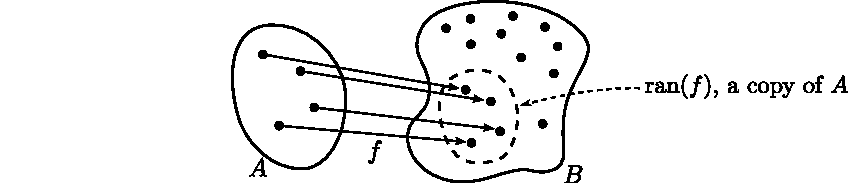
\includegraphics[scale=1]{img/embed.pdf}\end{center}
For $A$ to embed into $B$ like this,
it seems that $B$ must have at least as many elements as $A$, and $B$ can possibly have more elements that don't get mapped to.

A surjective function $g:A\rightarrow B$ associates the elements of $A$ to elements of $B$ in such a way that 
every element of $B$ has at least one element of $A$ mapping to it.
However, unless $g$ is also injective, some elements of $B$ can have multiple elements of $A$ mapping to them.
We can imagine that a surjection $g$ collapses some bunches of elements of $A$ onto all the individual elements of $B$.
\begin{center}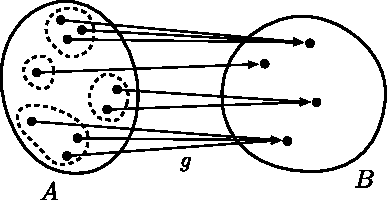
\includegraphics[scale=1]{img/collapse.pdf}\end{center}
For each element of $B$ to receive at least one arrow, it seems that $A$ must have at least as many elements as $B$,
and $A$ can possibly have more elements that get collapsed into some already-targeted elements of $B$.

A bijective function $h:A\rightarrow B$ associates all the elements of $A$ to all the elements of $B$ in a one-to-one way.
\begin{center}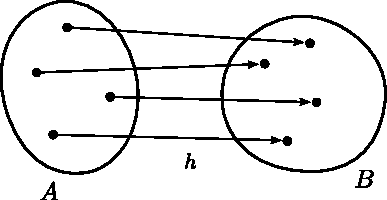
\includegraphics[scale=1]{img/collapse2.pdf}\end{center}
For a bijection to be possible, it seems that $A$ must have exactly as many elements as $B$.
If $A$ had too few elements, then some elements of $B$ would remain untargeted, ruling out surjectivity.
If $A$ had too many elements, then some collapsing would have to occur, ruling out injectivity.

This has been an imprecise discussion of some ideas that you can keep in mind for what is to come.

\DEFN{Cardinality\label{defn:card}}{
\begin{enumerate}[(1)]
\item $A\eqnm B\ \DARR\ \EXIST{f}{f:A\rightarrow B\ \AND\ \text{$f$ is a bijection onto $B$}}$.
\item $A\injex B\ \DARR\ \EXIST{f}{f:A\rightarrow B\ \AND\ \text{$f$ is injective}}$.
\item $A\injnobij B\ \DARR\ (A\injex B\ \AND\ \neg(A\eqnm B))$.
\end{enumerate}
}

When $A\eqnm B$, we say that $A$ and $B$ \emph{have the same cardinality}.
As suggsted by the informal discussion above, we can think of ``$A\eqnm B$'' as saying that
$A$ and $B$ have ``the same number of elements.''
%However, notice that there is no notion of ``number'' involved
%in the definition of ``$A\eqnm B$''.
However, notice that there is no mention of $\N$ or its elements in the definition of ``$A\eqnm B$''.
It is interesting that ``having the same number of elements'' can be defined without any reference to ``number.''

\THMPL{
\begin{enumerate}[(1)]
\item \label{thm:eqnm_props1}
$A\eqnm A$
\hfill (reflexivity for $\eqnm$)
\item \label{thm:eqnm_props2}
If $A\eqnm B$ then $B\eqnm A$.
\hfill (symmetry for $\eqnm$)
\item \label{thm:eqnm_props3}
If $A\eqnm B$ and $B\eqnm C$, then $A\eqnm C$.
\hfill (transitivity for $\eqnm$)
\end{enumerate}
}{
Proving \ref{thm:eqnm_props1} and \ref{thm:eqnm_props3} is \putExerciseHeading.
We prove \ref{thm:eqnm_props2} here.

Assume that $A\eqnm B$.
Get a bijection $f:A\rightarrow B$.
By Theorem \ref{thm:bij_inv}, the inverse $\rev{f}:B\rightarrow A$ is bijective.
Therefore $B\eqnm A$.
}{
\label{thm:eqnm_props}
}


\THMPL{
\begin{enumerate}[(1)]
\item \label{thm:injex_props1}
$A\injex A$
\hfill (reflexivity for $\injex$)
\item \label{thm:injex_props3}
If $A\injex B$ and $B\injex C$, then $A\injex C$.
\hfill (transitivity for $\injex$)
\end{enumerate}
}{
\putExerciseHeading.
}{
\label{thm:injex_props}
}

In the informal discussion at the beginning of this section, it is suggested that ``$A\injex B$''
is a way of saying that $B$ has at least as many elements as $A$.
If $B$ has at least as many elements as $A$, and $A$ has at least as many elements as $B$, then one would
expect that $A$ and $B$ must have the same amount of elements.
This turns out to be correct, but it is not so easy to prove.
This is the content of the next two theorems.

\THMNP{\label{thm:cbs_pre}Preliminary to Cantor-Schroeder-Bernstein}{
If $C\subseteq A$ and $A\injex C$, then $A\eqnm C$.
}{
Assume that $C\subseteq A$ and $A\injex C$.
Get an injection $f:A\rightarrow C$.
Let $S:\N\rightarrow \SUB{A}$ be the unique function that satisfies
$S(0)=A\setminus C$ and
$S(n+1)=f[S(n)]$ for all $n\in\N$.
Define
$$ D=\COLL{d}{\EXIST{n}{n\in\N\ \AND\ d\in S(n)}}. $$
Define
$$ g=\COLL{(a,f(a))}{a\in D} \ \cup\ \id{A\setminus D}. $$
We claim that $g:A\rightarrow C$ and $g$ is a bijection onto $C$.
Our claims are:
\begin{enumerate}[(1)]
\item \label{thm:csb_pre1} $g$ is a function.
\item \label{thm:csb_pre2} $\dom{g}=A$.
\item \label{thm:csb_pre3} $\ran{g} = C$.
\item \label{thm:csb_pre4} $g$ is injective.
\end{enumerate}
Once we prove these claims, we can conclude that $A\eqnm C$ and the theorem is proven.
We will establish a couple of useful facts along the way:
\begin{enumerate}[(1),resume]
\item \label{thm:csb_pre5}
$f[D]\subseteq D$.
\item \label{thm:csb_pre6}
For all $a\in A$, we have $g(a)=f(a)$ if $a\in D$ and we have $g(a)=a$ if $a\notin D$.
\end{enumerate}
\textit{Proof of Claim \ref{thm:csb_pre5}:}
Consider any $d\in D$; we must show that $f(d)\in D$.
Get $n\in\N$ such that $d\in S(n)$.
Then $f(d)\in f[S(n)]=S(n+1)$.
Therefore $f(d)\in D$.

\textit{Proof of Claim \ref{thm:csb_pre1}:}
Since $\COLL{(a,f(a))}{a\in D}$ is a subset of $f$, it is a function (see Exercise \ref{ex:restrict}).
Observe that $\dom{\COLL{(a,f(a))}{a\in D}}=D$ and $\dom{\id{A\setminus D}}=A\setminus D$
have empty intersection.
Since $g$ is the union of the two functions $\COLL{(a,f(a))}{a\in D}$ and $\id{A\setminus D}$,
and since the intersection of their domains is empty, it follows from Theorem \ref{thm:piecewise} that $g$ is a function.

\textit{Proof of Claim \ref{thm:csb_pre2}:}
Applying Exercise \ref{ex:domcup},
$$
\dom{g}\ =\ \dom{\COLL{(a,f(a))}{a\in D}}\ \cup\ \dom{\id{A\setminus D}}\ =\ D\cup(A\setminus D)\ =\ A.
$$

\textit{Proof of Claim \ref{thm:csb_pre6}:}
Consider any $a\in A$.
We will apply Theorem \ref{thm:ess_eval}.
If $a\in D$, then $(a,f(a))\in \COLL{(a,f(a))}{a\in D}\subseteq g$, so $f(a)=g(a)$.
If $a\notin D$, then $(a,a)\in\id{A\setminus D} \subseteq g$, so $a=g(a)$.

\textit{Proof of Claim \ref{thm:csb_pre3}:}
$\subseteq$:
Consider any $z\in\ran{g}$.
Get $x\in A$ such that $z=g(x)$.
Either $x\in D$ or $x\notin D$.

Case 1: Suppose that $x\in D$.
Then $z=g(x)=f(x)\in\ran{f}\subseteq C$.

Case 2: Suppose that $x\notin D$.
Then $z=g(x)=x \in A\setminus D$. If we had $z\notin C$, then we would have $z\in A\setminus C=S(0)\subseteq D$.
So it must be that $z\in C$.

In both cases we have shown that $z\in C$, so this proves that $\ran{g}\subseteq C$.

$\supseteq$:
Now consider any $z\in C$. Either $z\in D$ or $z\notin D$.

Case 1: Suppose that $z\notin D$. Then $z\in A\setminus D$, and so we have $z=g(z)\in\ran{g}$.

Case 2: Suppose that $z\in D$. Get $n\in \N$ such that $z\in S(n)$.
It cannot be that $n=0$, for then we would have $z\in S(0)=A\setminus C$, which contradicts the assumption $z\in C$.
Therefore we can get $m\in \N$ such that $n=m+1$ (Theorem \ref{thm:pred}).
Then $z\in S(m+1)=f[S(m)]$, so we can get a $d\in S(m)$ such that $z=f(d)$. Since $d\in D$, we have $g(d)=f(d)=z$.

In both cases we have shown that $z\in \ran{g}$, so this proves the claim.

\textit{Proof of Claim \ref{thm:csb_pre4}:}
Consider any $a,b\in A$ such that $g(a)=g(b)$.
We will show that $a=b$.
We consider four cases based on whether $a\in D$ and whether $b\in D$.

Case 1: Suppose that $a,b\in D$.
Then $f(a)=g(a)=g(b)=f(b)$, so it follows that $a=b$ due to the injectivity of $f$.

Case 2: Suppose that $a,b\notin D$.
Then $a=g(a)=g(b)=b$.

Case 3: Suppose that $a\in D$ and $b\notin D$.
Then $g(a)=f(a)$ and $g(b)=b$, so we have $f(a)=b$.
But this contradicts that $f[D]\subseteq D$, for we have $a\in D$ and $f(a)=b\notin D$.
It turns out that Case 3 is not possible.

Case 4: Suppose that $b\in D$ and $a\notin D$. This is Case 3 with $a$ and $b$ swapped.
Using the same argument, we see that Case 4 is not possible.
}

\THMNP{\label{thm:csb}Cantor-Schroeder-Bernstein, AKA Antisymmetry for $\injex$}{

If $A\injex B$ and $B\injex A$, then $A\eqnm B$. }{
Assume that $A\injex B$ and $B\injex A$.
Get an injection $f:A\rightarrow B$ and an injection $g:B\rightarrow A$.
Define $C=\ran{g}$. 
Observe that $g:B\rightarrow C$ is a bijection onto $C$. Therefore we have $B\eqnm C$.

Consider the composite $g\circ f :A\rightarrow A$.
By Theorem
\ref{thm:comp_inj_surj},
the composite $g\circ f$ is injective since $f$ and $g$ are injective.
Since $\ran{g\circ f}\subseteq\ran{g}=C$, we actually have $g\circ f :A\rightarrow C$.
That is, we have an injection from $A$ into a subset $C$ of $A$.
Theorem \ref{thm:cbs_pre} then applies and we conclude that $A\eqnm C$.

Since also $B\eqnm C$, we can apply symmetry and transitivity for $\eqnm$ to conclude that $A\eqnm B$.
}

\ex{\label{ex:subset_injex}Prove that if $A\subseteq B$, then $A\injex B$.}

\ex{Prove that if $A\eqnm B$ and $C\eqnm D$, then $A\times C \eqnm B\times D$.}

\THMP{If $A\injex B$, then there exists a surjection $g:B\rightarrow A$.}{
Assume that $A\injex B$.
Get an injection $f:A\rightarrow B$.
By Exercise
\ref{ex:inj_leftinv_real},
we can get a function $g:B\rightarrow A$ such that $g\circ f = \id{A}$.
It follows that $g\circ f$ is surjective, and so by Theorem
\ref{thm:comp_inj_surj}
we conclude that $g$ is surjective. 
}

\ex{\label{ex:choice_card}
Accepting Axiom \ref{ax:choice} just for this exercise, prove that if $f:A\rightarrow B$ is surjective onto $B$, then $B\injex A$.
}




\subsection{Finite Sets}

We next investigate finite sets.
It may be useful to be aware of the elements of $0,1,2,\ldots$ based on Definition \ref{def:numbers}:
\indented{
$0=\emptyset$\\
$1=\next{0}=0\cup\{0\}=\emptyset\cup\{0\}=\{0\}$\\
$2=\next{1}=1\cup\{1\}=\{0\}\cup\{1\}=\{0,1\}$\\
$3=\next{2}=2\cup\{2\}=\{0,1\}\cup\{2\}=\{0,1,2\}$\\
\ldots
}

\DEFN{Finiteness}{
\begin{enumerate}[(1)]
\item We say that $A$ \emph{has $n$ elements} iff $n\in\N$ and $A\eqnm n$.
\item A set is \emph{finite} iff it has $n$ elements for some $n\in\N$.
\item A set is \emph{infinite} iff it is not finite.
\end{enumerate}
}

\ex{Prove that a set is empty if and only if it has $0$ elements.}

\ex{Prove that a set is a singleton if and only if it has $1$ element.}

\ex{Prove that if $\{x,y\}$ has $2$ elements, then $x\neq y$.}


In some of the proofs to come, it is useful to be able to quickly get bijections that swap elements:

\THMNP{Element Swap\label{thm:swap}}{
If $p,q\in A$, then there is a bijection $f:A\rightarrow A$ such that $f(p)=q$ and $f(q)=p$.
}{
\putExerciseHeading.
Hint: Prove that $(\id{A}\setminus\{(p,p),(q,q)\})\cup \{(p,q),(q,p)\}$ works.
}

\THMNP{$\injex$ and $\leq$\label{thm:injex_leq}}{
If $n,m\in\N$, then $$n\injex m\ \DARR\ n\leq m.$$
}{
Assume that $n,m\in\N$.

$\Leftarrow$:
Assume that $n\leq m$.
Then whenever $k<n$, it follows that $k<m$.
In other words, $n\subseteq m$.
Therefore $n\injex m$, by Exercise \ref{ex:subset_injex}.

$\Rightarrow$:
We will prove by induction on $m$ that 
$$\ALL{n}{n\in\N\ \ARR\ (n\injex m\ARR n\leq m)},$$
for all $m\in\N$.
%It is important that the $n$ be quantified in the proposition on which we are doing induction. 

\BChead{}
Consider any $n\in\N$ such that $n\injex 0$.
Get an injection $f:n\rightarrow 0$.
We have $f\subseteq n\times \emptyset = \emptyset$, so $f=\emptyset$.
Therefore $n=\dom{f}=\emptyset=0$, and so $n\leq m$.

\IShead{}
Suppose that $m\in\N$ and $\ALL{n}{n\in\N\ \ARR\ (n\injex m\ARR n\leq m)}$.
Consider any $n\in\N$ such that $n\injex m+1$.
Get an injection $f:n\rightarrow (m+1)$.
Either $m\in\ran{f}$ or $m\notin\ran{f}$.

Case 1: Suppose that $m\notin\ran{f}$.
Then $f:n\rightarrow m$, so $n\injex m$.
By the induction hypothesis, it follows that $n\leq m$.
Therefore we also have $n\leq m+1$.

Case 2: Suppose that $m\in\ran{f}$.
Let $k$ be the unique element of $n$ such that $f(k)=m$.
Since $k<n$, we know that $0<n$, so we can get $s\in\N$ such that $n=s+1$.
Using Theorem \ref{thm:swap}, get a bijection $g:n\rightarrow n$ such that
$g(s)=k$ and $g(k)=s$.
Define $h=f\circ g$. Then we have that $h$ is injective,
$h:n\rightarrow m+1$, and $h(s)=f(g(s))=f(k)=m$.
Define $j=h\setminus\{(s,m)\}$.
Then $j$ is injective (see Exercise \ref{ex:subset_inj}), and
$j:(n\setminus\{s\})\rightarrow ((m+1)\setminus \{m\})$ (see Exercise \ref{ex:fn_deletion}).
Therefore we have $j:s\rightarrow m$
(see Exercise \ref{ex:setminus_decrement}).
Since we have found an injection from $s$ to $m$, we have $s\injex m$.
We may apply the induction hypothesis to $s$ to conclude that $s\leq m$.
It follows that $s+1\leq m+1$. That is, $n\leq m+1$.
}

\THMNP{$\eqnm$ and $=$ for Natural Numbers\label{thm:eqnm_eq}}{
If $n,m\in\N$, then $$n\eqnm m\ \DARR\ n = m.$$
}{
The implication ``$\Leftarrow$'' is just Axiom \ref{ax:eq_used} and Theorem \ref{thm:eqnm_props}.
For ``$\Rightarrow$'', assume that $n\eqnm m$. Then $m\eqnm n$ (Theorem \ref{thm:eqnm_props} again),
and so we have both $n\injex m$ and $m\injex n$. Applying Theorem \ref{thm:injex_leq} to both of these,
we get $n\leq m$ and $m\leq n$. It follows that $n=m$ (see Exercise \ref{ex:N_antisymmetry}).
}

\ex{\label{ex:injex_leq}Prove that if $X$ has $n$ elements, $Y$ has $m$ elements, and $X\injex Y$, then $n\leq m$.}

\ex{Assume
that $X$ has $n$ elements, $Y$ has $m$ elements, and $m<n$.
Prove that it is impossible for $f:X\rightarrow Y$ to be injective.
This result is called ``The Pigeonhole Principle.''
}

The next two theorems are special cases of Axiom \ref{ax:choice}.
Proofs are immediate if one chooses to accept Axiom \ref{ax:choice}.
We do not officially accept Axiom \ref{ax:choice} in these notes,
and so we provide proofs.

\THMNP{Finite Choice - Preliminary Version\label{thm:FC_prelim}}{
If $n\in\N$ and $f:A\rightarrow n$ surjectively, then there exists $g:n\rightarrow A$ such that $f\circ g=\id{n}$.
}{
We will prove that
$$
\ALL{A,f}{(\text{$f:A\rightarrow n$ surjectively})\ \ARR\ \EXIST{g}{(g:n\rightarrow A)\ \AND\ (f\circ g=\id{n})}}
$$
for all $n\in\N$, by doing induction on $n$.

\BChead{}
Consider any $A$ and $f$ such that $f:A\rightarrow 0$ surjectively.
Then we have $f\subseteq A\times\emptyset=\emptyset$, so $f=\emptyset$.
Therefore $A=\dom{f}=\emptyset$.
Define $g=\emptyset$.
Then $g:0\rightarrow A$, and $f\circ g=\emptyset=\id{\emptyset}=\id{0}$.

\IShead{}
Suppose that $n\in\N$ and that, for all $A,f$ such that $f:A\rightarrow n$ surjectively, there exists $g:n\rightarrow A$
such that $f\circ g=\id{n}$.
Now consider any $A$ and $f$ such that $f:A\rightarrow (n+1)$ surjectively.
Define $N=\rev{f}[\{n\}]$, and define
$f'=\COLL{(a,f(a))}{a\in A\setminus N}$.
Then we have $f':A\setminus N\rightarrow (n+1)$ (see Exercise \ref{ex:restrict2}).
We claim that $\ran{f'}=n$.

$\subseteq$:
To see that $\ran{f'}\subseteq n$, consider any $k\in\ran{f'}$.
Then $k\in (n+1)$.
To show that $k\in n$, we only need to show that $k\neq n$.
Get $a\in A\setminus N$ such that $f'(a)=k$.
Since $f'\subseteq f$, we also have $f(a)=f'(a)=k$.
If we had $k=n$, then we would have $a\in \rev{f}[\{n\}]=N$.
Therefore $k\neq n$.

$\supseteq$:
To see that $n\subseteq\ran{f'}$, consider any $k\in n$.
Then $k\in (n+1)$, so by the surjectivity of $f$ we can get some $a\in A$ such that $f(a)=k$.
If we had $a\in N$, then we would have $k=f(a)=n$, and this would lead to the impossible situation $n\in n$.
Therefore $a\in A\setminus N=\dom{f'}$.
Since $f'\subseteq f$, we then have $f'(a)=f(a)=k$.
Therefore $k\in \ran{f'}$.

Now we've established that $\ran{f'}=n$, so we have that $f':A\setminus N\rightarrow n$ and that $f'$ is surjective onto $n$.
Our induction hypothesis allows us to get $g:n\rightarrow A\setminus N$ such that $f'\circ g=\id{n}$.
Our remaining task is to construct a function $g':(n+1)\rightarrow A$ such that $f\circ g'=\id{n+1}$.
Since $f$ is surjective, the set $N$ is nonempty (see Exercise \ref{ex:surj_preimage}),
and so we can get $a_0$ such that $a_0\in N$. Define
$$
g'=g\cup\{(n,a_0)\}.
$$
We now claim that $g':(n+1)\rightarrow A$ and that $f\circ g'=\id{n+1}$. Once this is established, the induction step will be complete and the theorem will be proven.

To see that $g'$ is a function, we will use Theorem \ref{thm:piecewise}.
It is clear that $\{(n,a_0)\}$ is a function.
The intersection of $\dom{g}=n$ and $\dom{\{(n,a_0)\}}=\{n\}$
is empty by Theorem \ref{thm:irr_N}. By Theorem \ref{thm:piecewise}, we conclude that $g'$ is a function.

To see that $\dom{g'}=n+1$, we apply Exercise \ref{ex:domcup}:
$$
\dom{g'}=\dom{g\cup \{(n,a_0)\}}=\dom{g}\cup\dom{\{(n,a_0)\}}=n\cup\{n\}=n+1.
$$
To see that $\ran{g'}\subseteq A$, consider any $a\in\ran{g'}$.
Get $k\in(n+1)$ such that $g'(k)=a$.
Then either $k=n$ or $k\in n$.
In the case that $k=n$, we have $g'(k)=a_0\in N\subseteq A$.
In the case that $k\in n$, we have $g'(k)=g(k)\in\ran{g}\subseteq A\setminus N\subseteq A$.
In both cases, we ended up with $g'(k)\in A$. In other words, $a\in A$.

Finally, to see that $f\circ g'=\id{n+1}$ we consider any $k\in (n+1)$.
Then either $k=n$ or $k\in n$.

Case 1: Suppose that $k=n$. Then we have
$$
(f\circ g')(k) =
(f\circ g')(n) =
f(g'(n)) =
f(a_0)=n = k.
$$
Case 2: Suppose that $k\in n$.
Since $g\subseteq g'$ and $k\in\dom{g}$, we have $g(k)=g'(k)$.
Since $k\in\dom{g}$, we have $g(k)\in\ran{g}=A\setminus N = \dom{f'}$.
Since $f'\subseteq f$ and $g(k)\in\dom{f'}$, we have $f'(g(k))=f(g(k))$.
Putting these together, we have
$$
(f\circ g')(k) =
f(g'(k)) =
f(g(k)) = 
f'(g(k)) = 
(f'\circ g)(k)=
\id{n}(k)=
k.
$$
In both cases we ended up with 
$$(f\circ g')(k) = k = \id{n+1}(k), $$
so by Theorem \ref{thm:fn_eq} we conclude that $f\circ g'=\id{n+1}$.
}

\THMNP{Finite Choice\label{thm:FC}}{
If $X$ is finite and $f:A\rightarrow X$ surjectively, then there exists $g:X\rightarrow A$ such that $f\circ g=\id{X}$.
}{
Assume that $X$ is finite and $f:A\rightarrow X$ surjectively.
Get $n\in\N$ such that $X\eqnm\N$.
Get a bijection $h:X\rightarrow n$.
Then $h\circ f:A\rightarrow n$, and $h\circ f$ is surjective by Theorem \ref{thm:comp_inj_surj}.
Therefore we can apply Theorem \ref{thm:FC_prelim} to get some $j:n\rightarrow A$ such that
$(h\circ f)\circ j =\id{n}$.
Composing with $\rev{h}$ on the left and $h$ on the right
completes the proof; here are the details:
$$\begin{array}{llll}
\id{X} & = & \rev{h}\circ h \hspace{9em}                      & \text{(Theorem \ref{thm:inv_comp})}     \\
      & = & (\rev{h}\circ \id{n})\circ h                      & \text{(Theorem \ref{thm:ess_id})}       \\
      & = & (\rev{h}\circ ((h\circ f)\circ j))\circ h        &                                          \\
      & = & (\rev{h}\circ h) \circ (f \circ (j \circ h))     & \text{(Theorem \ref{thm:assoc_comp})}    \\
      & = & \id{X} \circ (f \circ (j \circ h))                & \text{(Theorem \ref{thm:inv_comp})}     \\
      & = & f \circ (j \circ h)                              & \text{(Theorem \ref{thm:ess_id})}.     
\end{array}$$
We have found a function $j\circ h:X\rightarrow A$ such that $f\circ (j\circ h)=\id{X}$.
}

Compare the following theorem to Exercise \ref{ex:choice_card}.

\THMPL{If $X$ is finite and $f:A\rightarrow X$ surjectively, then $X\injex A$.}{
Assume that $X$ is finite and $f:A\rightarrow X$ surjectively.
By Theorem \ref{thm:FC}, we can get $g:X\rightarrow A$ such that $f\circ g=\id{X}$.
By Theorem \ref{thm:comp_inj_surj}, the function $g$ must be injective.
}{
\label{thm:surj_finite}
}

\ex{Prove that if $n,m\in\N$ and there is a surjection $f:m\rightarrow n$, then $n\leq m$.}

\THMNP{Adding One Element\label{thm:card_add_one}}{
\begin{enumerate}[(1)]
\item\label{thm:card_add_one1}
If $X$ has $n$ elements and $a\notin X$, then $X\cup\{a\}$ has $n+1$ elements.
\item\label{thm:card_add_one2}
If $X$ is finite, then $X\cup\{a\}$ is finite.
\end{enumerate}
}{
Assume that $X$ has $n$ elements and $a\notin X$.
Get a bijection $f:X\rightarrow n$.
Define $f'=f\cup\{(a,n)\}$.

\putExerciseHeading: Prove that $f':X\cup\{a\}\rightarrow (n+1)$ and $f'$ is bijective.

\putExerciseHeading: Use \ref{thm:card_add_one1} to prove \ref{thm:card_add_one2}.
}

\THMNP{Subsets Inherit Finiteness - Preliminary Version\label{thm:subsets_inherit_finiteness_prelim}}{

If $n\in\N$ and $S\subseteq n$, then $S$ is finite.
}{
We will prove ``Every subset of $n$ is finite'' for all $n\in\N$ by doing induction on $n$.

\BChead{}
Consider any subset $S$ of $0$. Then $S=\emptyset$, so $S\eqnm 0$.

\IShead{}
Suppose that $n\in\N$, and that all subsets of $n$ are finite.
Consider any subset $S$ of $n+1$. Either $n\in S$ or $n\notin S$.

Case 1: Suppose that $n\notin S$.
Then $S\subseteq (n+1)\setminus\{n\} = n$.
The induction hypothesis then ensures that $S$ is finite.

Case 2: Suppose that $n\in S$.
Define $T=S\setminus\{n\}$.
Then $T\subseteq (n+1)\setminus\{n\} = n$,
so the induction hypothesis ensures that $T$ is finite.
It follows that $T\cup\{n\}$ is finite, by Theorem \ref{thm:card_add_one}.
Since $T\cup\{n\}=(S\setminus\{n\})\cup\{n\}=S$ (see Exercise \ref{ex:relcompfun} part \ref{ex:relcompfun1}),
we have shown that $S$ is finite.
}

\THMNP{Images Inherit Finiteness\label{thm:images_inherit_finiteness}}{
If $f:A\rightarrow B$, $X\subseteq A$, and $X$ is finite, then $f[X]$ is finite.
}{
Assume that $f:A\rightarrow B$, $X\subseteq A$, and $X$ is finite.
Get $n\in\N$ such that $X\eqnm n$.
Then $n\eqnm X$, so get a bijection $g:n\rightarrow X$.
We will argue that $f\circ g:n\rightarrow f[X]$ and that $f\circ g$ is a bijection onto $f[X]$.
This will prove that $n\eqnm f[X]$ and finish the proof of the theorem.

Since $X\subseteq A$, we do have $g:n\rightarrow A$, so $f\circ g:n\rightarrow B$.
Since $f$ and $g$ are injective, we know that $f\circ g$ is injective.

\putExerciseHeading: Prove that $\ran{f\circ g}=f[X]$.
}


\THMNP{Subsets Inherit Finiteness\label{thm:subsets_inherit_finiteness}}{If
$X$ is finite and $S\subseteq X$, then $S$ is finite.
}{
Assume that $X$ is finite and $S\subseteq X$.
Get $n\in\N$ such that $X\eqnm n$.
Get a bijection $f:X\rightarrow n$.
Then $f[S]\subseteq n$, so
$f[S]$ is finite by Theorem \ref{thm:subsets_inherit_finiteness_prelim}.
By Theorem \ref{thm:img_facts}, we have $S=\rev{f}[f[S]]$.
Since $\rev{f}$ is a function and $f[S]$ is finite, it follows from
Theorem \ref{thm:images_inherit_finiteness} that $\rev{f}[f[S]]$ is finite.
Therefore $S$ is finite.
}

\ex{
Here is an idea for a simpler way to prove Theorem \ref{thm:subsets_inherit_finiteness}:
\indented{
Assume that $X$ is finite and $S\subseteq X$. Then $S\injex X$
by Exercise \ref{ex:subset_injex}.
So by Exercise \ref{ex:injex_leq}, the set $S$ must have fewer elements than the finite set $X$.
Therefore $S$ is finite.
}
Why doesn't this approach work?
}



\THMNP{$\cup$ and $+$}{
If the set $X$ has $n$ elements, the set $Y$ has $m$ elements, and $X\cap Y=\emptyset$, then $X\cup Y$ has $n+m$ elements.
}{
\putExerciseHeading{} (Challenging).
Hint: Use induction and Theorem \ref{thm:card_add_one}.
Be precise about exactly what it is that you are proving by induction.
}


\THMP{Assume that $n\in\N$ and $f:n\rightarrow n$.
If $f$ is injective, then $f$ is surjective onto $n$.
}{
Assume that  $n\in\N$ and $f:n\rightarrow n$, and assume that $f$ is injective.
Suppose, for the sake of contradiction, that $f$ is not surjective.
Get $k\in n\setminus\ran{f}$.
Then $n$ is nonempty, so $n=m+1$ for some $m\in\N$ (Theorem \ref{thm:pred}).
Using Theorem \ref{thm:swap}, get a bijection $g:n\rightarrow n$ such that $g(k)=m$
and $g(m)=k$. Then $g\circ f :n\rightarrow n$ and $g\circ f$ is injective.
We will show that $\ran{g\circ f}\subseteq m$.

Consider any $z\in\ran{g\circ f}$.
We already have $z\in n=m+1$, so we just need to show that $z\neq m$ in order to conclude that $z\in m$. 
Get $\ell\in n$ such that $z=(g\circ f)(\ell)=g(f(\ell))$.
Suppose, for the sake of contradicition, that $z=m$.
Then $m=g(f(\ell))$ and $m=g(k)$, so since $g$ is injective it follows that $f(\ell)=k$.
But $k\notin\ran{f}$, so we have reached a contradiction.
Therefore $z$ cannot be $m$, and we may conclude that $z\in m$.

We have now shown that $\ran{g\circ f}\subseteq m$, so we have an injection $g\circ f :n\rightarrow m$.
Therefore we have $n\injex m$, and by Theorem \ref{thm:injex_leq} it follows that $n\leq m$.
But $n=m+1$, so we have reached a contradiction.
Therfore $f$ must be surjective.
}


\ex{Prove that if $X$ has $n+1$ elements and $x\in X$, then $X\setminus\{x\}$ has $n$ elements.}

\ex{(Challenging) In this exercise you will prove that every nonempty finite subset of $\N$ has a maximum.
Here are the relevant definitions:
\begin{itemize}
\item If $A\subseteq\N$ and $n\in\N$, then $n$ is an \emph{upper bound}
for $A$ iff $\ALL{k}{k\in A\,\ARR\,k\leq n}$.
\item If $A\subseteq \N$ and $n\in\N$, then $n$ is a \emph{maximum} for $A$ iff $n\in A$ and $n$ is an upper bound for $A$.
\end{itemize}
\begin{enumerate}
\item Prove that if a subset of $\N$ has a maximum, then the maximum is unique.
\item Prove that every finite subset of $\N$ has an upper bound.
Hint: Use induction to prove that
$$
\ALL{A}{(A\subseteq \N\ \AND\ A\eqnm n)\ \ARR\ \text{$A$ has an upper bound}}
$$
for all $n\in\N$.
\item Assume that $A$ is a nonempty finite subset of $\N$.
Let 
$$U=\COLL{n}{\text{$n\in\N$ and $n$ is an upper bound for $A$}}.$$
Use well-ordering (Theorem \ref{thm:wellord}) to argue that
$U$ has a minimum, and then prove that this minimum ends up being a maximum for $A$.
\end{enumerate}
}













\subsection{Infinite Sets}

\THMNP{Infinitude of $\N$}{
$\N$ is infinite.
}{
Suppose, for the sake of contradiciton, that $\N$ is finite.
Get $n\in\N$ such that $\N$ has $n$ elements.
Since $n+1\subseteq\N$, we have $n+1\injex\N$ (see Exercise \ref{ex:subset_injex}).
Since $n+1$ has $n+1$ elements, and $\N$ has $n$ elements, it follows that $n+1\leq n$
(see Exercise \ref{ex:injex_leq}). This is a contradiction.
Therefore $\N$ must be infinite.
}


\ex{Theorem \ref{thm:images_inherit_finiteness} does not work when ``image'' is replaced by ``preimage.''
Give an example of $A$, $B$, $f$, and $Y$ such that 
$f:A\rightarrow B$,\ \ $Y\subseteq B$,\ \ $Y$ is finite,\ \ and $\rev{f}[Y]$ is infinite.}


\DEFN{Countability}{A set $A$ is said to be \emph{countably infinite} iff $A\eqnm\N$.
}

We have now seen that two types of cardinalities can occur:
finite cardinality, where a set has the same cardinality as $n$
for some $n\in\N$, and infinite cardinality, where a set does not have the same cardinality as any $n\in\N$.
There are many possible finite cardinalities: those of $0$, $1$, $2$, etc.
These are all distinct cardinalities, by Theorem \ref{thm:eqnm_eq}.
Is there just one infinite cardinality, or are there also many infinite cardinalities?
If $A$ and $B$ are infinite sets, then do we necessarily have $A\eqnm B$?
Or could we actually have $A\injnobij B$ with $A$ and $B$ being infinite sets?

Let us start with the countably infinite set $\N$ and attempt to build up a set
with ``greater'' cardinality. 
Drawing inspiration from Theorem \ref{thm:card_add_one},
the first thing we might try is to add one element to $\N$.
This turns out not to affect the cardinality!

\THMNP{Hilbert's Hotel\label{thm:hotel}}{
$\next{\N}\eqnm\N$.
}{
Define $f=\addone{}\cup\{(\N,0)\}$.
(The diagram following this proof is a depiction of $f$.)
Since $\N\notin\N$ (see Exercise \ref{ex:NnotinN}), we may apply Theorem \ref{thm:piecewise} to
conclude that $f$ is a function.
We have
$$
\dom{f}=\dom{\addone{}}\cup\{\N\} = \N\cup\{\N\} =\next{\N},
$$
and we have
$$
\ran{f}=\ran{\addone{}}\cup\{0\}\subseteq\N,
$$
so $f:\next{\N}\rightarrow \N$.
We will show that $f$ is injective and surjective.

Suppose that $n,m\in\next{\N}$ and $f(n)=f(m)$.
In the case that $n,m\in\N$, we have $n+1=m+1$, so $n=m$.
In the case that $n,m\in\{\N\}$, we obviously have $n=m$.
In the case that $n\in\N$ and $m=\N$, we have $n+1=0$,
which is impossible.
Similarly, $n=\N$ and $m\in\N$ is impossible. Thus $f$ is injective.

Consider any $n\in\N$. If $n=0$, then $n=f(\N)$.
Otherwise, we can get $n'\in\N$ sich that $n=n'+1$. Then $n=f(n')$.
Thus $f$ is surjective.
}

\begin{center}
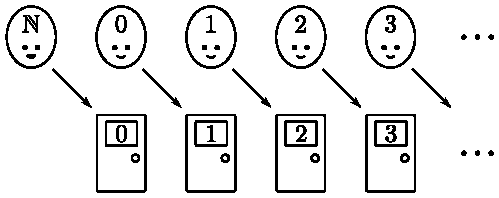
\includegraphics[scale=1]{img/hotel.pdf}
\end{center}

It follows from Theorem \ref{thm:hotel} that adding elements one-by-one to $\N$ is not going to yield new cardinalities.
All of the sets $\N$, $\next{\N}$, $\next{\next{N}}$, etc. have the same cardinality; they are all countably infinite.
The next thing one might try in order to produce a new cardinality is to ``double'' the set $\N$.
We can do this by considering the set $2\times \N$. This set consists of two distinct elements $(0,n)$ and $(1,n)$ for every $n\in\N$.
The set $2\times\N$ is sort of like a union of two separate copies of $\N$, so we might think it has ``twice as many'' elements.
And yet, as we are about to see in Theorem \ref{thm:doubleN}, the cardinality has still not changed!

To help us prove this, we will introduce the concepts of even and odd numbers.


\def\vsp{\vspace{0.3em}}
\DEFN{Even and Odd\label{defn:even}}{
\vsp
\begin{enumerate}[(1)]
\item $n$ is \emph{even} iff $n=k+k$ for some $k\in\N$. 
\item $n$ is \emph{odd} iff $n=k+k+1$ for some $k\in\N$.
\end{enumerate}
\vsp
}

\THMPL{Every natural number is either odd or even.}{
\putExerciseHeading. Hint: Induction.
}{
\label{thm:oddeven1}
}

\THMPL{A natural number cannot be both odd and even.}{
Suppose, for the sake of contradiction, that there exists a natural number which is both odd and even.
Let $n$ be the smallest such natural number (we are using Theorem \ref{thm:wellord}).
Get $\ell, k\in\N$ such that $n=\ell+\ell+1$ and $n=k+k$.
Since $n=(\ell+\ell)+1$, we cannot have $n=0$.
Since $n=k+k$ and $n\neq 0$, it must be that $k\neq 0$.
Get $k'\in\N$ such that $k=k'+1$.
Then 
$$k'+k'+1+1=(k'+1)+(k'+1)=k+k=n=\ell+\ell+1,$$
so $k'+k'+1=\ell+\ell$.
We see that $\ell+\ell$ is odd and even, and yet $\ell+\ell<\ell+\ell+1=n$.
This contradicts the fact that $n$ was the smallest odd-and-even natural number.
}{
\label{thm:oddeven2}
}

\THMPL{If $k,\ell\in\N$ and $k+k=\ell+\ell$ then $k=\ell$.}{
Assume that $k,\ell\in\N$ and $k+k=\ell+\ell$.
If $k<\ell$, then
$$ k+k < \ell+k < \ell+\ell $$
by Theorem \ref{thm:prop_plus},
so we cannot have $k<\ell$.
Similarly, we cannot have $\ell<k$. Thus $k=\ell$.
}{
\label{thm:oddeven3}
}

\THMNP{Doubling Countable Infinity\label{thm:doubleN}}{
$2\times \N\eqnm\N$.
}{
Define
$$
f=\COLL{((0,n),n+n)}{n\in\N}\cup\COLL{((1,n),n+n+1)}{n\in\N}.
$$
With the help of Theorem \ref{thm:piecewise}, it is straightforward to show that $f:2\times\N\rightarrow\N$.
The diagram following this proof is a depiction of $f$.

To prove that $f$ is injective, assume that $(i,n),(i',n')\in 2\times\N$ and $f((i,n))=f((i',n'))$.
We cannot have $i=0$ and $i'=1$, for then we would have $n+n=n'+n'+1$,
and this contadicts Theorem \ref{thm:oddeven2}. Similarly, we cannot have $i=1$ and $i'=0$.
This leaves two cases.

Case 1: Suppose that $i=i'=0$. Then $n+n=n'+n'$, so $n=n'$ by Theorem \ref{thm:oddeven3}.
Thus $(i,n)=(i',n')$.

Case 2: Suppose that $i=i'=1$. Then $n+n+1=n'+n'+1$, so $n+n=n'+n'$.
It follows from Theorem \ref{thm:oddeven3} that $n=n'$. Thus $(i,n)=(i',n')$.

Since we get $(i,n)=(i',n')$ in all cases, we conclude that $f$ is injective.

To prove that $f$ is surjective, consider any $k\in\N$.
By Theorem \ref{thm:oddeven1}, $k$ is either odd or even.

Case 1: Suppose that $k$ is odd. Get $n\in\N$ such that $k=n+n+1$.
Then $k=f((1,n))$, so $k\in\ran{f}$.

Case 2: Suppose that $k$ is even. Get $n\in\N$ such that $k=n+n$.
Then $k=f((0,n))$, so $k\in\ran{f}$.

Since we get $k\in\ran{f}$ either way, we conclude that $f$ is surjective onto $\N$.
Therefore $f$ is a bijection, and we have shown that $2\times\N\eqnm\N$.
}

\begin{center}
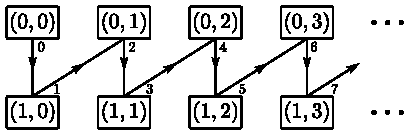
\includegraphics[scale=1]{img/sawtooth.pdf}
\end{center}

So apparently mushing together two copies of $\N$ still leaves us with the same ``amount'' of elements-- only countably infinitely many.
Okay, what if we mush together \emph{countably infinitely} many copies of the countably infinite set $\N$?
What if instead of $2\times \N$ we consider $\N\times \N$? This contains an entire copy of $\N$ for each element of $\N$!
And yet, as we are about to see, it is still only countably infinite!

\THMNP{Squaring Countable Infinity\label{thm:squareN}}{
$\N\times \N\eqnm\N$.
}{
We will start by constructing a useful function $a:\N\rightarrow\N$,
and then we will construct a bijection $f:\N\rightarrow \N\times\N$.

First, define $r:\N\times\N\rightarrow\N\times\N$ by
$$
r((k,n))=(k+(n+1),n+1)
$$
for all $k,n\in\N$. Let $a':\N\rightarrow\N\times\N$ be the unique function that satisfies
$$
\begin{array}{ll}
a'(0)=(0,0)\hspace{2em}&\text{and}\\
a'(n+1)=r(a'(n))\hspace{2em}&\text{for all $n\in\N$.}
\end{array}
$$
Define $a=\COLL{(n,k)}{(n,(k,n))\in a'}$.

To see that $a$ is a function, suppose that $(n,k),(n,k')\in a$.
Then $(n,(k,n)),(n',(k',n))\in a'$. Since $a'$ is a function, we have
$(k,n)=(k',n)$. It follows that $k=k'$.
Thus $a$ is a function. 

Notice the following about $a$:
\indented{
Fact 1: $(0,0)\in a$. This is because $(0,(0,0))\in a'$.\\
Fact 2: For any $n\in\N$ and any $k$, if $(n,k)\in a$, then $(n+1,k+(n+1))\in a$.
This is because for any $n\in\N$ and any $k$ we have
$$
(n,(k,n))\in a'\Rightarrow (n+1,(k+(n+1),n+1))=(n+1,r((k,n)))\in a'.
$$
}%
One consequence of Fact 1 is that $0\in\dom{a}$.
One consequence of Fact 2 is that for any $n\in\N$, if $n\in\dom{a}$ then $n+1\in\dom{a}$.
It follows by induction that $\N\subseteq\dom{a}$.
It is clear from the definition of $a$ that $\dom{a}\subseteq\N$ and that $\ran{a}\subseteq\N$, so
we now have $a:\N\rightarrow\N$.
We may now express Facts 1 and 2 as follows:
\indented{
Fact 1: $a(0)=0$.\\
Fact 2: For all $n\in\N$, we have $a(n+1)=a(n)+(n+1)$.
}%
The idea is that $a$ counts the number of dots in these triangular portions of a dot grid:
\begin{center}
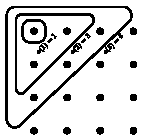
\includegraphics[scale=1.5]{img/dotgrid.pdf}
\end{center}
We will need one more useful fact about $a$ before we construct our bijection:
\indented{Fact 3: For $n,n'\in\N$, if $n<n'$ then $a(n)+n<a(n')$.}
To prove this, we fix $n\in\N$ and do induction on $n'$.
The base case, $n'=0$, is vacuous. Suppose, for the induction step, that 
$n'\in\N$ and $n<n'\Rightarrow a(n)+n<a(n')$.
Assume that $n<n'+1$.
We must prove that $a(n)+n<a(n'+1)$.
We have $n\leq n'$, so we may proceed by cases as follows.

Case 1: Suppose that $n=n'$. Then
$$
a(n)+n<a(n)+(n+1)=a(n+1)=a(n'+1).
$$
Case 2: Suppose that $n<n'$. Then we have $a(n)+n<a(n')$ by the induction hypothesis, so
$$
a(n)+n<a(n')<a(n')+(n'+1)=a(n'+1).
$$
We completed the induction step in both cases, so Fact 3 is proven.

Finally, we construct our bijection for the sake of proving $\N\eqnm\N\times\N$.
Define
\begin{align*}
f&=\COLL{(a(n)+i,(i,j))}{i,j,n\in\N\ \AND\ i+j=n}\\
&=\COLL{p}{\EXIST{i,j,n}{p=(a(n)+i,(i,j))\ \AND\ i,j,n\in\N\ \AND\ i+j=n}}.
\end{align*}
The diagram following this proof is a depiction of $f$.
It is clear that $f\subseteq\N\times(\N\times\N)$, so we are left needing to prove four things:
\indented{
that $f$ is a function,\\
that $\N\subseteq\dom{f}$,\\
that $f$ is injective,\\
and that $f$ is surjective onto $\N\times\N$.
}%
To prove that $f$ is a function, consider any $(x,y),(x,y')\in f$.
Get $i,j,n\in\N$ such that $i+j=n$ and $(x,y)=(a(n)+i,(i,j))$.
Get $i',j',n'\in\N$ such that $i'+j'=n'$ and $(x,y')=(a(n')+i',(i',j'))$.
Then $a(n)+i=x=a(n')+i'$.
Now if we had $n<n'$, then it would follow from Fact 3 above that $a(n)+n<a(n')$.
But since $i\leq i+j=n$, this would lead to
$$
a(n)+i\leq a(n)+n<a(n')\leq a(n')+i',
$$
so it cannot be that $n<n'$.
By a similar argument, it cannot be that $n'<n$.
Therefore we must have $n=n'$.
We then get $i=i'$ from 
$$a(n)+i=a(n')+i'=a(n)+i'.$$
And finally we get $j=j'$ from
$$
i+j=n=n'=i'+j'=i+j'.
$$
Therefore $y=(i,j)=(i',j')=y'$,
and we have proven that $f$ is a function.

To prove that $\N\subseteq\dom{f}$, we will use induction.
Since $0=a(0)+0$, we have $(0,(0,0))\in f$.
Therefore $0\in\dom{f}$.
For an induction step, suppose that $m\in\N$ and $m\in\dom{f}$.
Get $y$ such that $(m,y)\in f$.
Get $i,j,n\in\N$ such that $i+j=n$ and $(m,y)=(a(n)+i,(i,j))$.
Then $m=a(n)+i$. We have $i\leq i+j=n$, so either $i<n$ or $i=n$.

Case 1: Suppose that $i<n$.
Then $0<j$, for if $j=0$ then $i=n$.
Get $j'\in\N$ such that $j=j'+1$.
Define $i'=i+1$.
Then 
$$i'+j'=(i+1)+j'=i+(j'+1)=i+j=n,$$
so $(a(n)+i',(i',j'))\in f$. Thus
$$
m+1=(a(n)+i)+1=a(n)+i'\in\dom{f}.
$$
Case 2:
Suppose that $i=n$. Then $m=a(n)+n$, so $m+1=a(n)+(n+1)=a(n+1)$.
Define $i'=0$ and $j'=n+1$.
Then we have $i'+j'=n+1$, so $(a(n+1)+i',(i',j'))\in f$.
Thus
$$
m+1=a(n+1)=a(n+1)+i'\in\dom{f}.
$$
We completed the induction step in both cases, so by induction we have proven that $\N\subseteq\dom{f}$.

We now have $f:\N\rightarrow\N\times\N$, and it remains to prove that $f$ is bijective.

To prove that $f$ is injective, consider any $x,x'\in\dom{f}$
such that $f(x)=f(x')$.
Get $i,j,n\in\N$ such that $i+j=n$ and $(x,f(x))=(a(n)+i,(i,j))$.
Get $i',j',n'\in\N$ such that $i'+j'=n'$ and $(x',f(x'))=(a(n')+i',(i',j'))$.
We have $(i,j)=f(x)=f(x')=(i',j')$, so $i=i'$, $j=j'$, and
$$n=i+j=i'+j'=n'.$$
Since $i=i'$ and $n=n'$, we have
$$
x=a(n)+i=a(n')+i'=x'.
$$
Therefore $f$ is injective.

To prove that $f$ is surjective, consider any $(i,j)\in\N\times\N$.
Define $n=i+j$.
Then we have $f(a(n)+i)=(i,j)$, so $f$ is surjective onto $\N\times\N$.

We have shown that there exists a bijection $f:\N\rightarrow\N\times\N$; we conclude that $\N\eqnm\N\times\N$.
}

\begin{center}
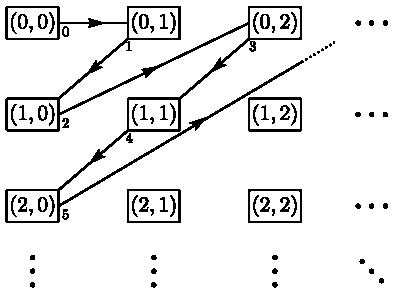
\includegraphics[scale=1]{img/gridbij.pdf}
\end{center}


So even 
putting together countably infinitely many copies of a countably infinite set still does not yield a new cardinality--
only another countably infinite set.
It is starting to look like there is only one way for a set to be infinite, from the standpoint of cardinality.
This turns out to be dead wrong, as we will see in Theorem \ref{thm:cantor}!

\ex{\label{ex:injexsub}
Prove that $A\injex \SUB{A}$.
}


\THMNP{Cantor's Theorem\label{thm:cantor}}{
There does not exist a surjection $f:A\rightarrow\SUB{A}$.
}{
Suppose for the sake of contradiction that $f:A\rightarrow\SUB{A}$
is surjective onto $\SUB{A}$.
Define
$$
C=\COLL{a}{a\in A\ \AND\ a\notin f(a)}.
$$
Then $C\in\SUB{A}$, so
since $f$ is surjective we can get some $b\in A$ such that $f(b)=C$.
Either $b\in C$ or $b\notin C$.

Case 1: Suppose that $b\in C$.
Then $b\notin f(b)=C$. This a contradiction.

Case 2: Suppose that $b\notin C$.
Then $b\in f(b)=C$. This is a contradiction.
}

\DEFN{Uncountability}{
A set $A$ is said to be \emph{uncountably infinite} iff it is infinite, but it is not countably infinite.
}

Given Theorem \ref{thm:cantor} and Exercise \ref{ex:injexsub}, we see that
there are many ways for a set to be infinite, from the standpoint of cardinality.
We have the countably infinite set $\N$, and then we have
an unending ladder of uncountably infinite cardinalities beyond that:
$$
\N\injnobij\SUB{\N}\injnobij\SUB{\SUB{\N}}\injnobij\SUB{\SUB{\SUB{\N}}}\injnobij\cdots
$$

\def\A{\mathscr{A}}
\def\F{\mathscr{F}}
\def\Ap{\A^*}

\ex{ (Challenging)
In this exercise, you will prove that $\N$ is the ``smallest'' infinite set there is, from the standpoint of cardinality.
You will prove that given any infinite set $A$, one has $\N\injex A$.
As far as I know, this requires Axiom \ref{ax:choice}, so you should accept Axiom \ref{ax:choice} just for this exercise.
\begin{itemize}
\item Assume that $A$ is an infinite set.
\item Define $\A{}=\COLL{S}{S\subseteq A\ \AND\ S\neq\emptyset}=\SUB{A}\setminus\{\emptyset\}$, the set of nonempty subsets of $A$.
\item Define $\Ap{}=\COLL{(a,S)}{(a,S)\in A\times\A{}\ \AND\ a\in S}$. Elements of $\Ap{}$ are sometimes called \emph{pointed sets},
since they are pairs consisting of a set and a ``point'' in the set.
\item Define $\pi_1=\COLL{((a,S),a)}{(a,S)\in\Ap}$ and $\pi_2=\COLL{((a,S),S)}{(a,S)\in\Ap}$.
Then we have $\pi_1:\Ap{}\rightarrow A$ and $\pi_2:\Ap{}\rightarrow \A{}$.
These two functions are called \emph{projections}.
\end{itemize}
\begin{enumerate}
\item Prove that $\pi_1$ and $\pi_2$ are surjective.
\end{enumerate}
\begin{itemize}
\item We may now use Axiom \ref{ax:choice} to get some $g:\A{}\rightarrow\Ap{}$ such that $\pi_2\circ g=\id{\A{}}$.
\item Define $c=\pi_1\circ g$. Then $c:\A{}\rightarrow A$.
\end{itemize}
\begin{enumerate}[resume]
\item Prove that for all $S\in\A{}$, we have $c(S)\in S$.
Thus the function $c$ serves to ``choose'' an element of each $S\in\A{}$. This is why 
Axiom \ref{ax:choice} is called the Axiom of Choice.
\end{enumerate}
\begin{itemize}
\item Define $\F=\COLL{S}{S\subseteq A\ \AND\ \text{$S$ is finite}}$, the set of finite subsets of $A$.
\item The goal now is to construct $h:\N\rightarrow A\times\F$ such that
\indented{
$h(0)=(a_0,\emptyset)$, where $a_0\in A$,\\
$h(1)=(a_1,\{a_0\})$, where $a_1\in A\setminus\{a_0\}$,\\
$h(2)=(a_2,\{a_0,a_1\})$, where $a_2\in A\setminus\{a_0,a_1\}$,\\
etc.
}
To do this, we first define a function $r:A\times \F\rightarrow A\times\F$ by
$$
r((a,F))=(c(A\setminus (F\cup\{a\})),F\cup\{a\})
$$
for all $(a,F)\in A\times\F$.
\end{itemize}
\begin{enumerate}[resume]
\item 
Prove that this definition of $r$ is okay by showing that
for any $(a,F)\in A\times\F$, we have $A\setminus (F\cup\{a\})\in \A{}$ and $F\cup\{a\}\in\F$.
\end{enumerate}
\begin{itemize}
\item Now let $h:\N\rightarrow A\times \F{}$ be the unique function that satisfies
\indented{
$h(0)=(c(A),\emptyset)$ \hspace{2em} (note that $A\in\A{}$, because we assumed $A$ is infinite) \hspace{2em} and\\
$h(n+1)=r(h(n))$ for all $n\in\N$.
}
\item
Define $\pi_1'=\COLL{((a,F),a)}{(a,H)\in A\times \F{}}$ and $\pi_2'=\COLL{((a,F),F)}{(a,F)\in A\times \F{}}$.
Then $\pi_1':A\times\F{}\rightarrow A$ and $\pi_2':A\times\F{}\rightarrow\F{}$.
\item
Define $f=\pi_1'\circ h$ and $H=\pi_2'\circ h$.
Then $f:\N\rightarrow A$ and $H:\N\rightarrow \F{}$.
\end{itemize}
\begin{enumerate}[resume]
\item Prove that
$f(0)=c(A)$,  $H(0)=\emptyset$, and
$$ H(n+1)=H(n)\cup\{f(n)\} \hspace{2em} \text{and}\hspace{2em} f(n+1)=c(A\setminus H(n+1))$$
for all $n\in\N$.
\item Prove that for all $n\in\N$, $f(n)\notin H(n)$.
\item Prove that for all $n,m\in\N$,  $n<m \ARR f(n)\in H(m)$.
\item Prove that $f$ is injective.
\end{enumerate}
\begin{itemize}
\item Thus $\N\injex A$.
\end{itemize}
}








\subsection{Relations}

Given a set $A$, one can think of subsets of $A$ as \emph{unary predicates}
about elements of $A$.
For example if one defines $G=\COLL{g}{\text{$g\in A$ and $g$ is green}}$,
then, for elements of $A$, to ``be green'' is to ``be an element of $G$.''
This would be a \emph{unary} predicate becuase the proposition ``$g$ is green''
has just one variable in it-- it is true or false depending on what $g$ is.
The set $G$ is an object which represents the concept of ``being green'' for elements of $A$.

In a similar vein, one can think of subsets of $A\times A$ as \emph{binary} predicates
about elements of $A$. For example if one defines
$L=\COLL{(x,y)}{\text{$x,y\in A$ and $x$ loves $y$}}$,
then, for elements $x,y$ of $A$, we have ``$x$ loves $y$'' if and only if we have $(x,y)\in L$.
The set $L$ is an object which represents the concept of ``loving'' for elements of $A$.
Instead of writing ``$(x,y)\in L$,'' we will often use an infix notation and write ``$xLy$.''
In this context, $L$ is a \emph{relation}.

\DEFN{Relations}{
\begin{enumerate}[(1)]
\item $R$ is a \emph{relation on $A$} if and only if  $R\subseteq A\times A$.
\item When $R$ is a relation on $A$, we write ``$xRy$'' to mean ``$(x,y)\in R$.''
\end{enumerate}
}

Instead of using letters like $R$ or $L$ for variables that stand for relations, we will often
use the symbol ``$\REL$''. This is just
because it looks pretty in the infix notation: $(x,y)\in\,\,\REL$ if and only if $x\REL y$.
Bear in mind that even though the symbol $\REL$ is not a letter of the alphabet, it is
still a \emph{variable} and not a constant. What ``$\REL$'' refers to and what assumptions about
``$\REL$'' are available all depends on context.

\DEFN{Adjectives for Relations\label{defn:reln_adj}}{
Assume that $\REL\,\,\subseteq A\times A$.
\begin{enumerate}[(1)]
\item $\REL$ is \emph{reflexive} on $A$ iff $a\REL a$ for all $a\in A$.
\item $\REL$ is \emph{symmetric} iff $a\REL b\ \ARR\ b\REL a$ for all $a,b$.
\item $\REL$ is \emph{transitive} iff $((a\REL b)\ \AND\ (b\REL c))\ \ARR\ (a\REL c)$ for all $a,b,c$.
\item $\REL$ is \emph{antisymmetric} iff $((a\REL b)\ \AND\ (b\REL a))\ \ARR\ (a=b)$ for all $a,b$.
\item $\REL$ is \emph{total} on $A$ iff $(a\REL b)\ \OR\ (b\REL a)$ for all $a,b\in A$.
\end{enumerate}
}

\DEFN{Special Kinds of Relations}{
Assume that $\REL\,\,\subseteq A\times A$.
\begin{enumerate}[(1)]
\item $\REL$ is a \emph{preorder} on $A$ iff it is reflexive on $A$ and transitive.
\item $\REL$ is a \emph{partial order} on $A$ iff it is an \emph{antisymmetric} preorder on $A$.
\item $\REL$ is a \emph{total order} on $A$ iff it is a \emph{total} partial order on $A$.
\item $\REL$ is an \emph{equivalence relation} on $A$ iff it is a \emph{symmetric} preorder on $A$.
\end{enumerate}
}

\ex{Assume that $\REL$ is a relation on $A$.
\begin{enumerate}
\item Prove that $\REL$ is a preorder on $A$ if and only if $\id{A}\subseteq\,\,\REL$ and $\REL\circ\REL\,\,\subseteq\,\, \REL$.
\item Prove that if $\REL$ is a preorder on $A$ then $\REL\circ\REL\,\,=\,\, \REL$.
\item Prove that $\REL$ is an equivalence relation on $A$ if and only if
$\id{A}\subseteq\,\,\REL$,
$\REL\circ\REL\,\,\subseteq\,\, \REL$,
and $\rev{\REL}\subseteq\,\,\REL$.
\item Prove that if $\REL$ is an equivalence relation on $A$ then
$\REL\circ\REL\,\,=\,\, \REL$
and $\rev{\REL}=\,\,\REL$.
\item Prove that $\REL$ is total on $A$ if and only if $\REL\cup\,\,\rev{\REL}=A\times A$.
\end{enumerate}
}

When $A$ is a small finite set, we can depict relations $\REL$ on $A$ by drawing a labeled dot for each element of $A$
and then drawing an arrow from the the dot labeled $x$ to the dot labeled $y$ whenever $x\REL y$.
For example,
\begin{center}
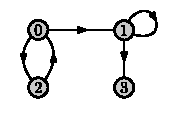
\includegraphics{img/relations_gfx/00000.pdf}
\end{center}
depicts the relation $\{(0,1),(1,1),(1,3),(0,2),(2,0)\}$
on the set $\{0,1,2,3\}$.

\newcommand{\exline}[1]{\item \raisebox{-0.8cm}{\includegraphics{img/relations_gfx/#1.pdf}}}

\ex{Consider the following relations on $\{0,1,2,3\}$:

\begin{minipage}{\textwidth}
\begin{enumerate*}[(a), itemjoin=\hspace{2cm}] 
\exline{11100}
\exline{10110}
\exline{11000}
\exline{01000}
\exline{10101}
\exline{01100}
\exline{00000}
\exline{00110}
\exline{10000}
\exline{10001}
\exline{10010}
\exline{empty}
\exline{10100}
\exline{00100}
\exline{11110}
\exline{00010}
\exline{11101}
\exline{10011}
\exline{01110}
\exline{10111}
\end{enumerate*}
\end{minipage}

Answer the questions below. You do not need to prove anything.
\begin{enumerate}
\item Which relations are reflexive on $\{0,1,2,3\}$?
\item Which relations are symmetric?
\item Which relations are transitive?
\item Which relations are antisymmetric?
\item Which relations are total on $\{0,1,2,3\}$?
\item Which relations are preorders  on $\{0,1,2,3\}$?
\item Which relations are partial orders on $\{0,1,2,3\}$?
\item Which relations are total orders on $\{0,1,2,3\}$?
\item Which relations are equivalence relations on $\{0,1,2,3\}$?
\end{enumerate}
}

\ex{
Assume that $\REL$ is a relation on $A$.
\begin{enumerate}
\item Prove that if $\REL$ is total on $A$, then $\REL$ is reflexive on $A$.
\item Prove that if $\REL$ is symmetric and antisymmetric, then $\REL\,\,\subseteq\id{A}$.
\item Prove that $\id{A}$ is the only relation on $A$ which is reflexive, symmetric, and antisymmetric.
\item Prove that $A\times A$ is the only relation on $A$ which is symmetric and total.
\end{enumerate}
}

\ex{
For each of the following relations on $\N$, determine which of the adjectives in Definition \ref{defn:reln_adj} apply.
Point out which relations are equivalence relations and which are partial orders.
\begin{enumerate}
\item $\REL\,\,=\COLL{(n,m)}{n,m\in\N\ \AND\ n\leq m}$
\item $\REL\,\,=\COLL{(n,m)}{n,m\in\N\ \AND\ n< m}$
\item $\REL\,\,=\COLL{(n,m)}{n,m\in\N\ \AND\ n= m}$
\item $\REL\,\,=\COLL{(n,m)}{n,m\in\N\ \AND\ 4<n+m}$
\item $\REL\,\,=\COLL{(n,m)}{n,m\in\N\ \AND\ n\leq m+m}$
\item $\REL\,\,=\COLL{(n,m)}{n,m\in\N\ \AND\ n+n\leq m}$
\item $\REL\,\,=\COLL{(n,n+1)}{n,m\in\N}$
\item $\REL\,\,=\COLL{(n,n+1)}{n,m\in\N} \cup \COLL{(n+1,n)}{n,m\in\N}$
\item $\REL\,\,=\COLL{(n,m)}{n,m\in\N\ \text{ and $n+m$ is even}}$\ \ (recall Definition \ref{defn:even})
\end{enumerate}
}

\ex{
\begin{enumerate}
\item Define $\REL\,\,=\COLL{(X,Y)}{X,Y\subseteq A\ \AND\ X\subseteq Y}$. 
Prove that $\REL$ is a partial order on $\SUB{A}$.
\item Define $\REL\,\,=\COLL{(X,Y)}{X,Y\subseteq A\ \AND\ X\injex Y}$
(recall Definition \ref{defn:card}).
Prove that $\REL$ is a partial order on $\SUB{A}$.
(Hint: Much of the hard work has been done by previous theorems that you can reference.)
\item Define $\REL\,\,=\COLL{(X,Y)}{X,Y\subseteq A\ \AND\ X\eqnm Y}$.
Prove that $\REL$ is an equivalence relation on $\SUB{A}$.
\item For each of the following relations on $\SUB{A}$, determine which of the adjectives in Definition \ref{defn:reln_adj} apply:
\begin{enumerate}
\item $\REL\,\,=\COLL{(X,Y)}{X,Y\subseteq A\ \AND\ X\cap Y = \emptyset}$
\item $\REL\,\,=\COLL{(X,Y)}{X,Y\subseteq A\ \AND\ X\cap Y \neq \emptyset}$
\end{enumerate}
\end{enumerate}
}


\renewcommand{\exline}[1]{\item \raisebox{-1.3cm}{\includegraphics{img/relations_gfx/#1.pdf}}}

\ex{\label{ex:eqblobs}
For each of the following relations on $7$, add a minimal number of arrows to turn them into equivalence relations.
So do nothing if the given relation is already an equivalence relation, and otherwise draw in only the arrows that need to be included in order to ensure
reflexivity, symmetry, and transitivity.

\begin{minipage}{\textwidth}
\begin{enumerate*}[(a), itemjoin=\hspace{2cm}]
\exline{er06}
\exline{er01}
\exline{er02}
\exline{er03}
\exline{er04}
\exline{er05}
\end{enumerate*}
\end{minipage}
}

After doing Exercise \ref{ex:eqblobs}, you might notice that an equivalence relation seems to partition a set into batches,
where everything any any given batch is connected to everything else in the same batch, and where there are no connections between different batches.
These batches are called \emph{equivalence classes}.

\DEFN{Equivalence Class}{Assume that $\REL{}$ is an equivalence relation on $A$ and $a\in A$. Then we define
$$
\CLASS{a}{\REL} = \COLL{x}{x\REL{}a}
$$
and we call this the \emph{equivalence class of $a$}, or the \emph{equivalence class of $a$ modulo $\REL$}.
If the relation involved is clear from context, then we may simply write $\CLASS{a}{}$ instead of $\CLASS{a}{\REL}$.
}

\ex{For each part of Exercise \ref{ex:eqblobs}, after you have added the arrows that are needed to have an equivalence relation, 
determine the equivalence classes $\CLASS{0}{}$ and $\CLASS{1}{}$.
(``Determine'' means ``list the elements.'')
}


\note{Equivlance relations and partitions.
Consider defining $\Z$ using equivalence relations.
Consider talking about partial orders, and other sorts of relations.
Consider introducing ideas of $\sup$ and $\inf$.}



\appendix

\section{Fixing the Bug}

\note{Explain what is broken about the membership axiom. Outline some of the changes that need to be made to align the development here to proper NBG set theory,
going through how the membership axiom can be repaired, and what new axioms need to be introduced to let pretty much the same machinery run.
}

\section{Maps}

\note{Describe the category of sets and the theorems from the functions chapter that can be re-construed as properties of the category of sets.
Emphasize the importance of ``fixing the bug'' for the purpose of doing category theory.
Mention that there are many categories.}

% "codomain" and morphisms and the category viewpoint



%\section{Philosophy}

%\note{Provide references for interesting topics in the philosophy of mathematics that are approachable after studying the material here.}

% was everything really a set this whole time and we were just ignorant? um no
% benacerraf points from "what numbers could not be"


\end{document}



